\begin{refsection} 
 
\chapter{Solar Cells} \label{chapter:slme} 
 
\setlength{\epigraphwidth}{3in} 
\epigraph{\textit{``We are star stuff harvesting sunlight.”}}{Carl Sagan} 
\vspace{3em} 
 
Solar cell technology is a rapidly developing field, largely driven by the 
discovery of cheaper and more efficient materials. However, the conventional 
search for materials that can serve as absorber layers in photovoltaic devices is both expensive and 
time consuming. Modern high-throughput computational methods have the power to 
screen large amounts of materials relatively quickly, providing valuable 
information that allows experimental work to focus on promising compounds. In 
order to accurately screen materials, a proper selection metric is required. 
The spectroscopic limited maximum efficiency (SLME) attempts to improve upon 
the traditional Shockley-Queisser (SQ) limit by including the first-principles 
calculated absorption spectrum of the material in the determination of the 
efficiency. It also allows researchers to investigate the thickness dependence 
of the efficiency, which is particularly interesting for thin-film solar cell 
research.
 
In this chapter I give an overview of my work on solar cell absorber materials, 
which was largely performed during the first year of my PhD. After a brief 
introduction, the chapter
starts by explaining the basic working principles of a solar cell 
in Section~\ref{slme:sec-basics}. Next, Section~\ref{slme:sec-metric} 
continues by discussing the SLME, as well as its predecessor, the Shockley 
Queisser limit. In Section~\ref{slme:sec-CuAu}, this selection metric is 
applied to compare the potential of a range of ternary I-III-VI$_2$ compounds 
in both the CuAu-like and the chalcopyrite phase. Finally, some crucial 
aspects of our chosen selection metric are investigated in 
Section~\ref{slme:sec-analysis}. 
 
\pagebreak 

\section{Introduction} 
 
Nearly all sources of energy found on earth are in some way derived from the 
sun. Both animals and plants depend on solar energy to produce the heat and 
sustenance they need to survive. Fossil fuels are nothing more than long 
buried organisms, exposed to millions of years of heat and pressure in the 
earth's crust. Wind energy would not exist without the air currents that are a 
product of solar heated air and the rotation of the earth. Solar cells are 
\textit{photovoltaic} (PV) devices that try to directly convert the sun's 
light into electricity, by absorbing the incoming photons and using the 
resulting energy to create a current of moving electrons. They have the 
advantage of being a renewable source of clean energy, whose application can 
be much more distributed than more conventional sources of 
electricity~\cite{Marsden2011}. 
 
The first practical photovoltaic devices were constructed in the 1950s. Over 
the course of the next decades, solar cell technology was mainly developed by 
the space industry, which required a reliable source of energy for its 
satellite applications. In the 1980s, solar cells received an increased amount 
of attention due to the oil crisis and a growing demand for power supply in 
remote areas that are not connected to the electricity grid. More recently, 
the threat of global warming has expanded the interest in sustainable energy 
sources. Advances in technology have increased the efficiency and longevity of 
solar cells, while reducing the costs of production and maintenance. 
Moreover, governments around the world have started initiatives to increase the 
percentage of the world's renewable energy supply. 
Figure~\ref{slme:fig-pv_evo} shows the results of these efforts. We can see 
that the PV market has increased significantly over the past decade, now 
contributing 5.9\% of the total global (grid-connected) electrical energy production. 
An important caveat here is that the production and recycling of solar modules 
also requires energy, and has an environmental impact. With regards to the 
production, Bhandari et al.~\cite{Bhandari2015} report an energy payback 
time (EPBT) of 1 to 4.1 years depending on the type of module. Considering 
a lifetime of 25 years for the average solar cell, efficient end-of-life (EOL) 
strategies will have to developed to ensure the sustainability of photovoltaic 
devices~\cite{Chowdhury2020}.
 
\begin{figure}[hb]  
\centering 
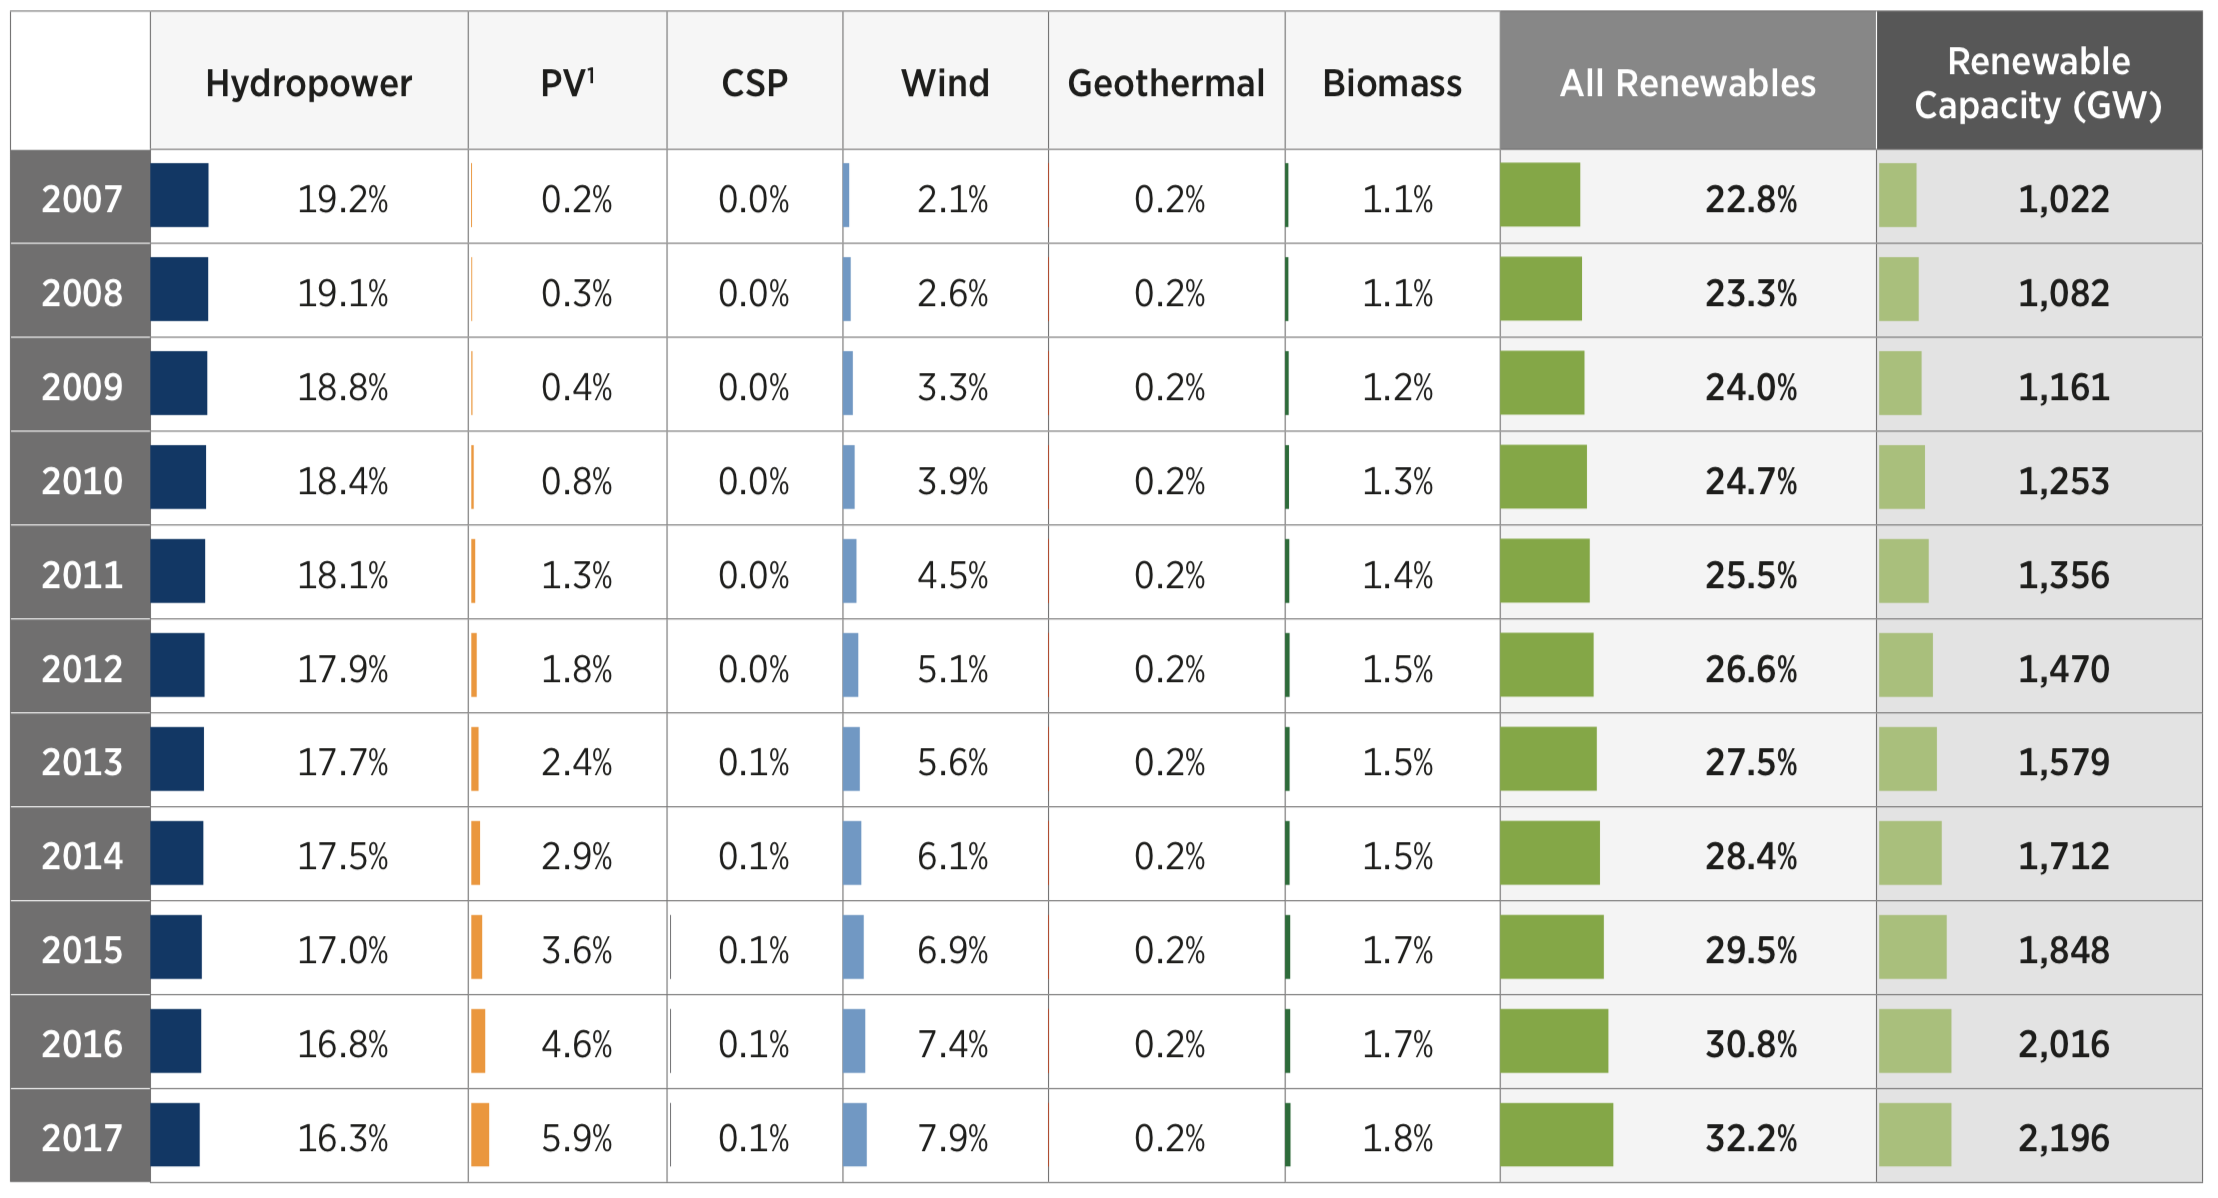
\includegraphics[width=0.9\textwidth]{\figurepath/slme/pv-evo.png} 
\caption{Renewable electricity as a percentage of the total installed global 
electricity capacity. Note that the PV numbers here are for grid-connected production only, represented by the index~1. CSP stands for concentrated solar power. Taken from~\cite{NREL2017}.}
\label{slme:fig-pv_evo}  
\end{figure}  

Although the growth of the PV market is promising, continued efforts must be 
made to increase the share of renewable energy in the global energy 
production. In order to make solar cells more economically competitive with 
conventional sources of electricity, new materials have to be found that 
either increase the efficiency or lower the cost of PV devices. In this 
chapter, we investigate a selection metric that determines the potential of a 
material for solar cell applications. 

%The Shockley-Queisser limit~\cite{Shockley1961} is one of the most well-known 
% metrics to determine the maximum efficiency an absorber material can produce 
% in a single-junction solar cell. It was proposed in 1961 and provides a direct 
% relation between the band gap of a material and its maximum possible 
% efficiency. More recently, Yu and Zunger expanded on the work of Shockley and 
% Queisser by introducing the Spectroscopic Limited Maximum 
% Efficiency~\cite{Yu2012} (SLME), which takes the absorption coefficient and 
% thickness into consideration for the calculation of the maximum efficiency. 
% The SLME has since been used to investigate the potential of photovoltaic 
% absorber materials such as perovskites~\cite{Meng2016}, direct band gap 
% silicon crystals~\cite{Lee2014}, chalcogenides, and other materials. In our 
% recent work on CuAu-like~\cite{Bercx2016} and Stannite~\cite{Sarmadian2016} 
% structures, we also used the SLME to study the efficiency of these materials 
% in the context of thin film solar cells. Interestingly, we found several 
% materials with an SLME above the Shockley-Queisser limit, and identified that 
% this is due to the lower recombination current obtained for the material at 
% lower thicknesses. 
 
\section{Solar Cell Basics} \label{slme:sec-basics} 
 
This section discusses the basics of solar cells, starting from a presentation 
of the solar spectrum and the absorption coefficient. It continues by 
explaining recombination effects, an important limiting factor for solar cell 
efficiency. The P-N junction, as well as the relevant equations, are the next 
topic of this section. Finally, we present the working principles of the solar 
cell, as well as a discussion of its I-V characteristic, which is essential 
for understanding the selection metrics introduced in the 
Section~\ref{slme:sec-metric}. 
 
\subsection{Solar Spectrum} 
 
Before discussing the operation of solar cells, we briefly take a look at the 
solar spectrum itself (Fig.~\ref{slme:fig-solar}). In good approximation, the 
sun emits electromagnetic radiation as a black body, a perfectly absorbing 
mass whose emission spectrum is determined by Planck's radiation 
law~\cite{Planck1901}. Due to the influence of the sun's atmosphere, the 
spectral distribution that reaches the outside of earth's atmosphere differs 
from the ideal black-body spectrum. Before reaching the planetary surface, the 
incoming radiation intensity is further attenuated by various scattering and 
absorption effects~\cite{Bird1986}. The degree of attenuation depends on the 
angle at which the light enters the atmosphere. The solar spectra are usually 
classified by their \textit{Air Mass} (AM)~\cite{Green1981}: 
\begin{minipage}{1\textwidth} 
\begin{minipage}{0.4\textwidth} 
\begin{equation} 
\text{Air Mass} = \frac{1}{\cos \theta_z}, 
\end{equation} 
\end{minipage} 
\begin{minipage}{0.6\textwidth} 
\centering 
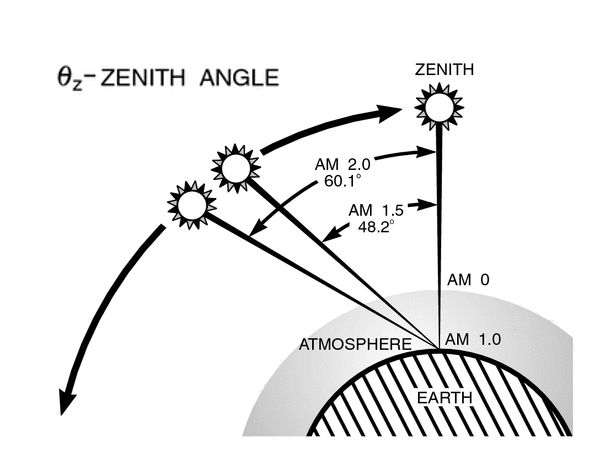
\includegraphics[width=1\textwidth]{\figurepath/slme/airmass.png} 
\captionof{figure}{\label{slme:fig-Airmass}Relation between zenith and Air 
Mass~\cite{Newport2015}.} 
\end{minipage} 
\end{minipage} 
\vspace{0.2in}\\ 
where $\theta_z$ is the zenith angle of the incoming 
light~(Fig.~\ref{slme:fig-Airmass}). The use of these standard spectra allows 
the performance of devices to be judged fairly, by exposing them to the same 
agreed-upon spectrum. In this work, we use the AM 1.5G irradiance spectrum for 
all of our calculations, which is a good representation of the illumination conditions on a tilted flat PV array. The `G' stands for global tilt and
refers to the angle between the normal of the surface and the direction of the 
incoming sunlight. 
 
\begin{figure}[ht]
\captionsetup{width=0.9\textwidth}
\centering 
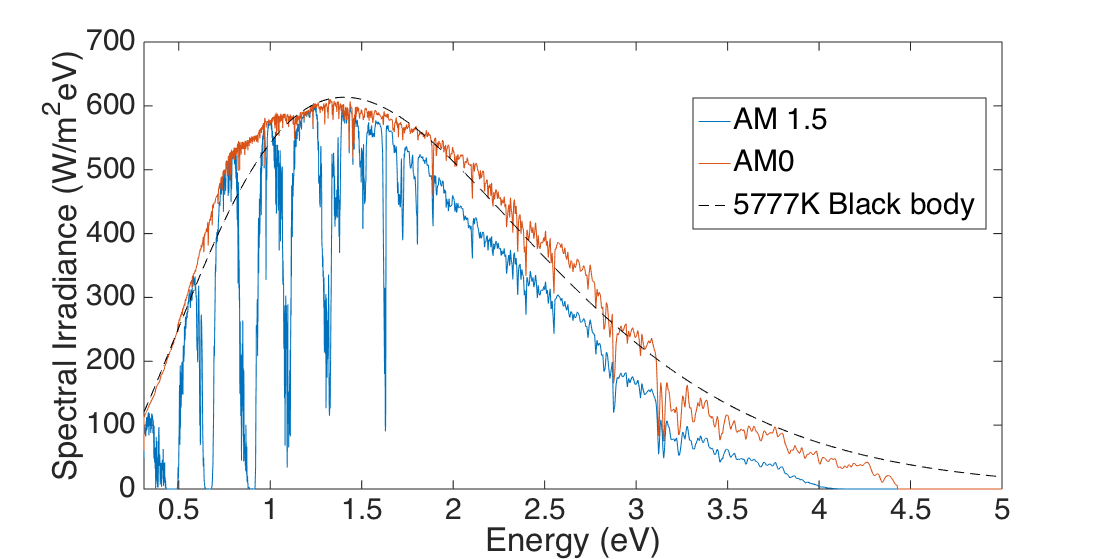
\includegraphics[width=0.75\textwidth]{\figurepath/slme/SolarSpectrum.png} 
\caption{\label{slme:fig-solar} Solar Spectra for the extraterrestial AM 0 
(orange) and AM 1.5 (blue) measurements. A black-body spectrum is added as a 
reference point. Data taken from~\cite{International2012}.} 
\end{figure} 
 
\subsection{Absorption}\label{slme:sec-absorption} 
 
When light passes through a semiconductor, a fraction of the photons is 
absorbed by the material, which causes the system to undergo a transition into 
an excited state. An example of such a higher energy state is an electron that 
is excited from the valence band (VB) to the conduction band (CB). When an 
electron undergoes this transition, it leaves behind a space in the valence 
band for other electrons to move into. Rather than keeping track of the 
valence band electrons, the movement of the empty space is usually represented 
by a positively charged particle, referred to as a \textit{hole}. In this 
framework, the absorption of light is considered as the creation of an 
electron-hole pair, called an \textit{exciton}, through the annihilation of an 
incoming photon. If the electron-hole pair can be separated, they become 
free charge carriers that can move through the semiconductor. 
 
\begin{wrapfigure}{l}{0.4\textwidth}
\centering 
\captionsetup{width=0.9\textwidth} 
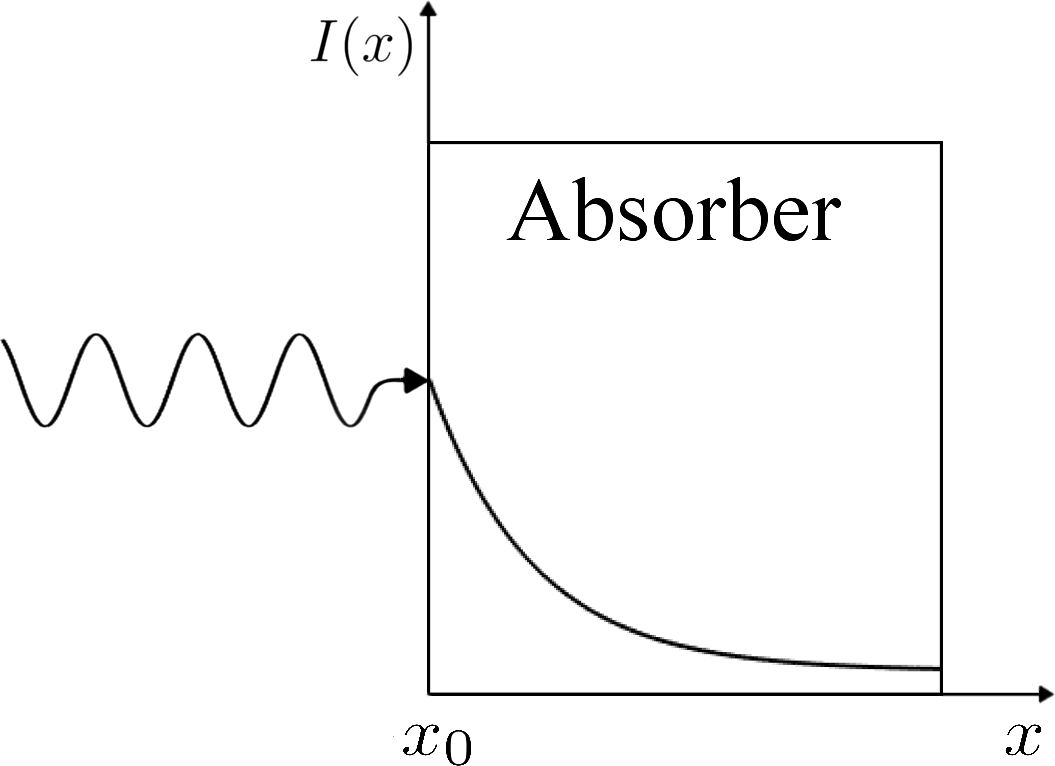
\includegraphics[width=\textwidth]{\figurepath/slme/Intensity.png} 
\caption{\label{slme:fig-intensity} Attenuation of the incoming light.} 
\end{wrapfigure} 
 
The absorption process is essential for the generation of carriers that 
produce the current in photovoltaic devices. The strength of the absorption of 
a material for photons of energy $E$ is described by the \textit{absorption 
coefficient} $\alpha(E)$, which determines the attenuation of the incoming 
monochromatic light~\cite{Green1981}: 
\begin{equation}\label{slme:eq-intensity} 
I(x) = I(x_0)e^{-\alpha(E) (x - x_0)}, 
\end{equation} 
where $I(x_0)$ is the intensity upon entering the 
semiconductor~(Fig.~\ref{slme:fig-intensity}). The absorption coefficient is 
related to the extinction coefficient $\hat{k}$, which is defined as the 
imaginary part of the complex index of refraction $\hat{n}_c(E)=n(E)+ik(E)$: 
\begin{equation}\label{slme:eq-absorption} 
\alpha (E)= \frac{4 \pi E \cdot k(E)}{h c}, 
\end{equation} 
where $h$ is Planck's constant and $c$ is the speed of light. Both the real 
and imaginary parts of the index of refraction can be calculated from the 
dielectric tensor, see Section~\ref{dft:sec-linear}. 
 
\begin{figure}[ht]  
\centering 
\begin{subfigure}{0.50\textwidth} 
\centering 
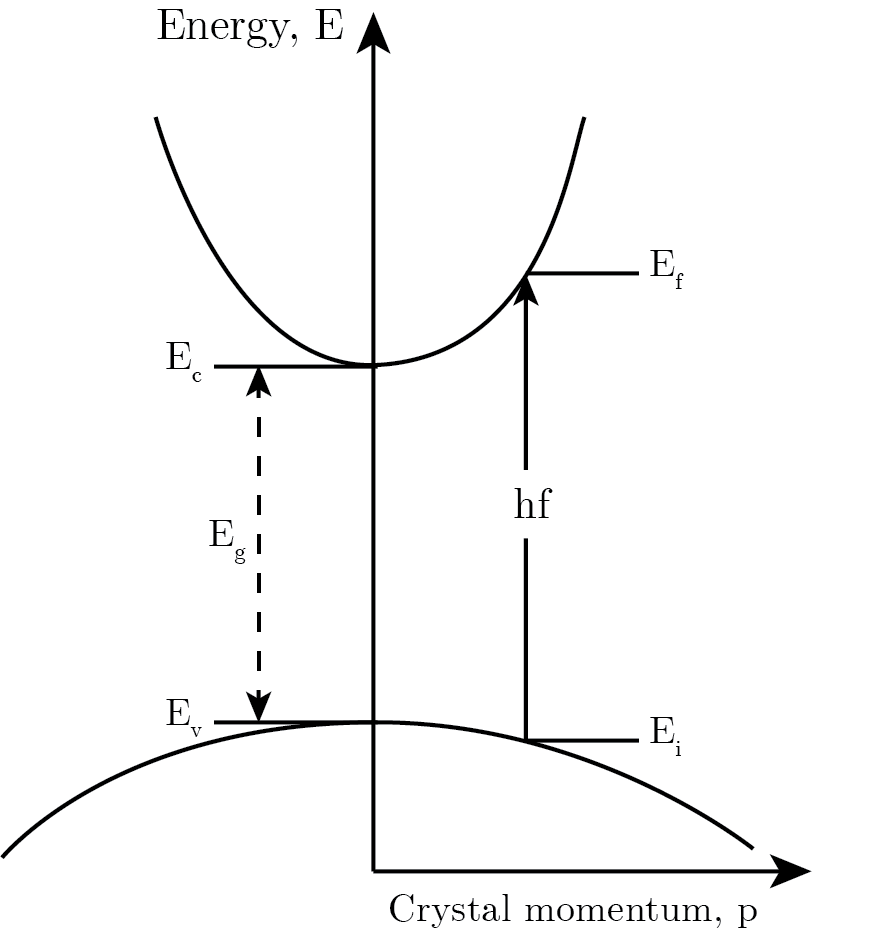
\includegraphics[width=0.9\linewidth]{\figurepath/slme/Direct.png} 
\caption{} 
\end{subfigure}% 
\begin{subfigure}{0.50\textwidth} 
\centering 
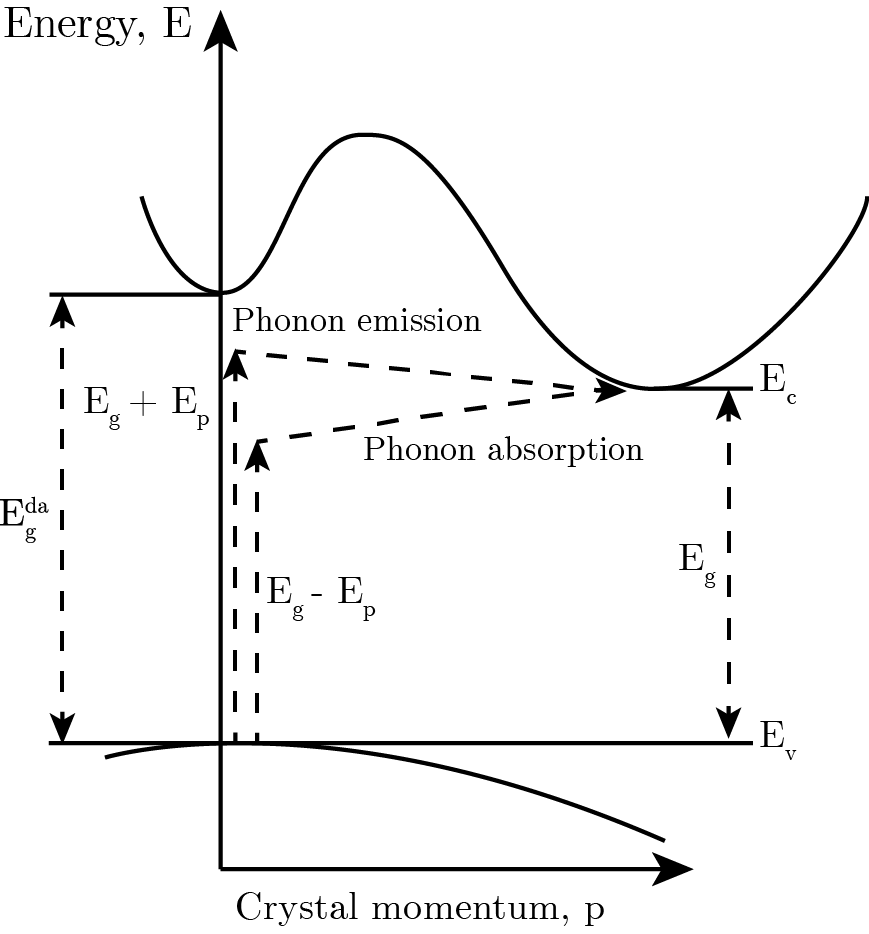
\includegraphics[width=0.9\linewidth]{\figurepath/slme/Indirect.png} 
\caption{} 
\end{subfigure} 
\caption{\label{slme:fig-abstypes}Direct (a) and indirect (b) absorption. 
Adapted from \cite{Green1981}.} 
\end{figure} 
 
An important distinction to make here is the difference 
between \textit{direct} and \textit{indirect} transitions 
(Fig.~\ref{slme:fig-abstypes}). When a photon is absorbed to excite an 
electron to a higher energy level, there must be a conservation of energy and 
momentum. For direct transitions, the electron absorbs both the photon energy 
and momentum, the latter of which is very small. However, for indirect band 
gap semiconductors, the minimum energy of the conduction band occurs at a very 
different value of the crystal momentum than the maximum energy of the valence 
band. In this case, absorption of photons with energies close to the band gap 
involves the participation of phonons -- quasiparticles describing the 
mechanical vibrations in the crystal -- in order to provide the necessary change 
in momentum. For these materials, it is useful to make a distinction between 
the \textit{fundamental} band gap $E_g$ and the \textit{direct allowed} band 
gap $E_g^{da}$, the latter of which is defined as the minimal difference in 
energy of the valence and conduction band at the same crystal momentum. 
 
\subsection{Recombination}\label{slme:sec-recombination} 
 
The electrons that are excited to the conduction band in a semiconductor are 
in a metastable state and eventually return back to the valence band, 
effectively also removing the holes they left after their transition to the 
conduction band. This process is called \textit{recombination}. The lifetime 
of an electron-hole pair depends on the rate of the different recombination 
mechanisms present in the semiconductor material. In this work, we make a 
distinction between three types of recombination: 
 
\begin{wrapfigure}[10]{r}{0.50\textwidth}
\vspace{-3em}
\centering 
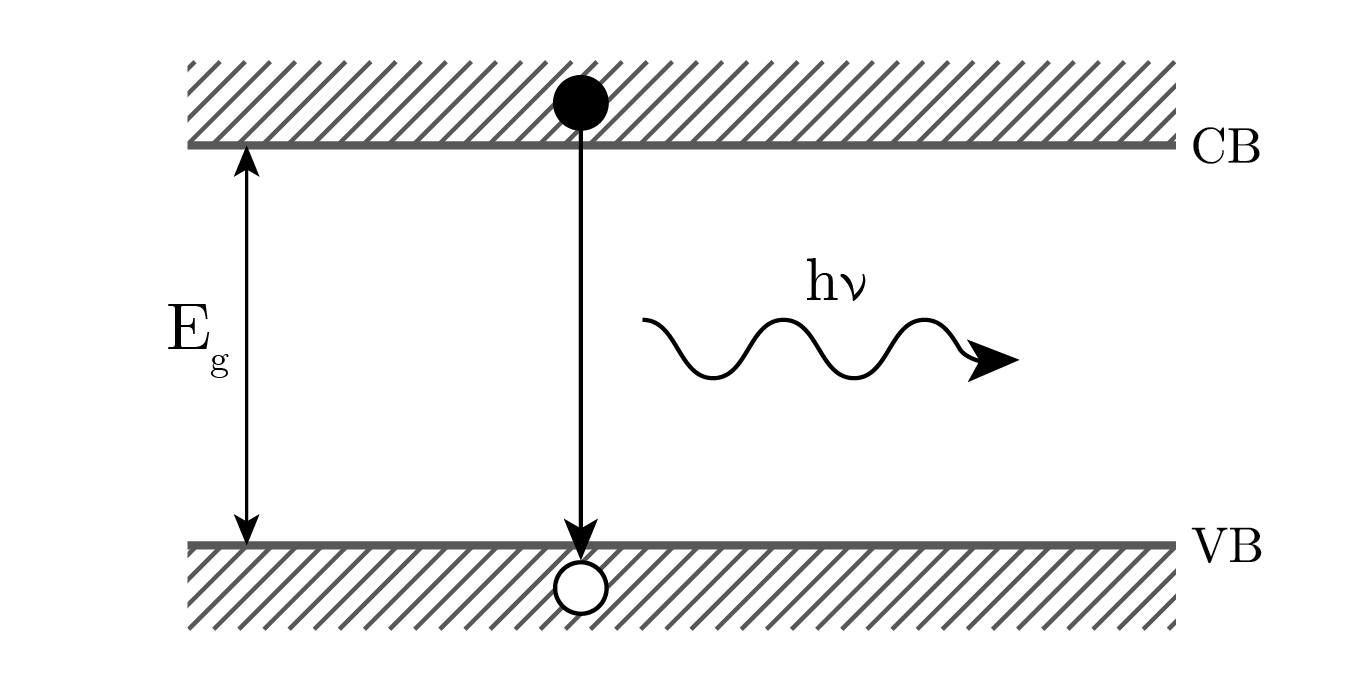
\includegraphics[width=\textwidth]{\figurepath/slme/RadRec.png} 
\caption{\label{slme:fig-radrec} Radiative Recombination.} 
\end{wrapfigure}
\vspace{1em}
\textbf{Radiative Recombination} is an interband process that can be 
considered the reverse of the absorption process. An excited electron in the 
conduction band recombines with a hole in the valence band, producing a photon 
which is emitted by the diode~(Fig.~\ref{slme:fig-radrec}). The energy of the 
photon is given by $h \nu = E_c - E_v = E_g$. This recombination mechanism is 
prevalent in direct band gap absorbers such as GaAs, a material used for the 
design of light-emitting diodes~\cite{Green1981}. 

\pagebreak[4]
\textbf{Auger Recombination}~\cite{Auger1923} is a three particle 
mechanism, where the energy produced by the electron-hole recombination is 
transferred to another electron (either in the conduction or valence band), 
instead of emitting a photon. The second electron then returns back to its 
original energy via thermal relaxation~(Fig.~\ref{slme:fig-augerrec}). Since 
no light is emitted in this process, it is often referred to as 
\textit{non-radiative} recombination. This type of recombination is dominant 
in indirect band gap materials, of which the most important example is 
silicon~\cite{Nilsson1973}. 
\begin{figure}[ht]  
\centering
\captionsetup{width=0.9\textwidth} 
\begin{subfigure}{0.50\textwidth} 
\centering 
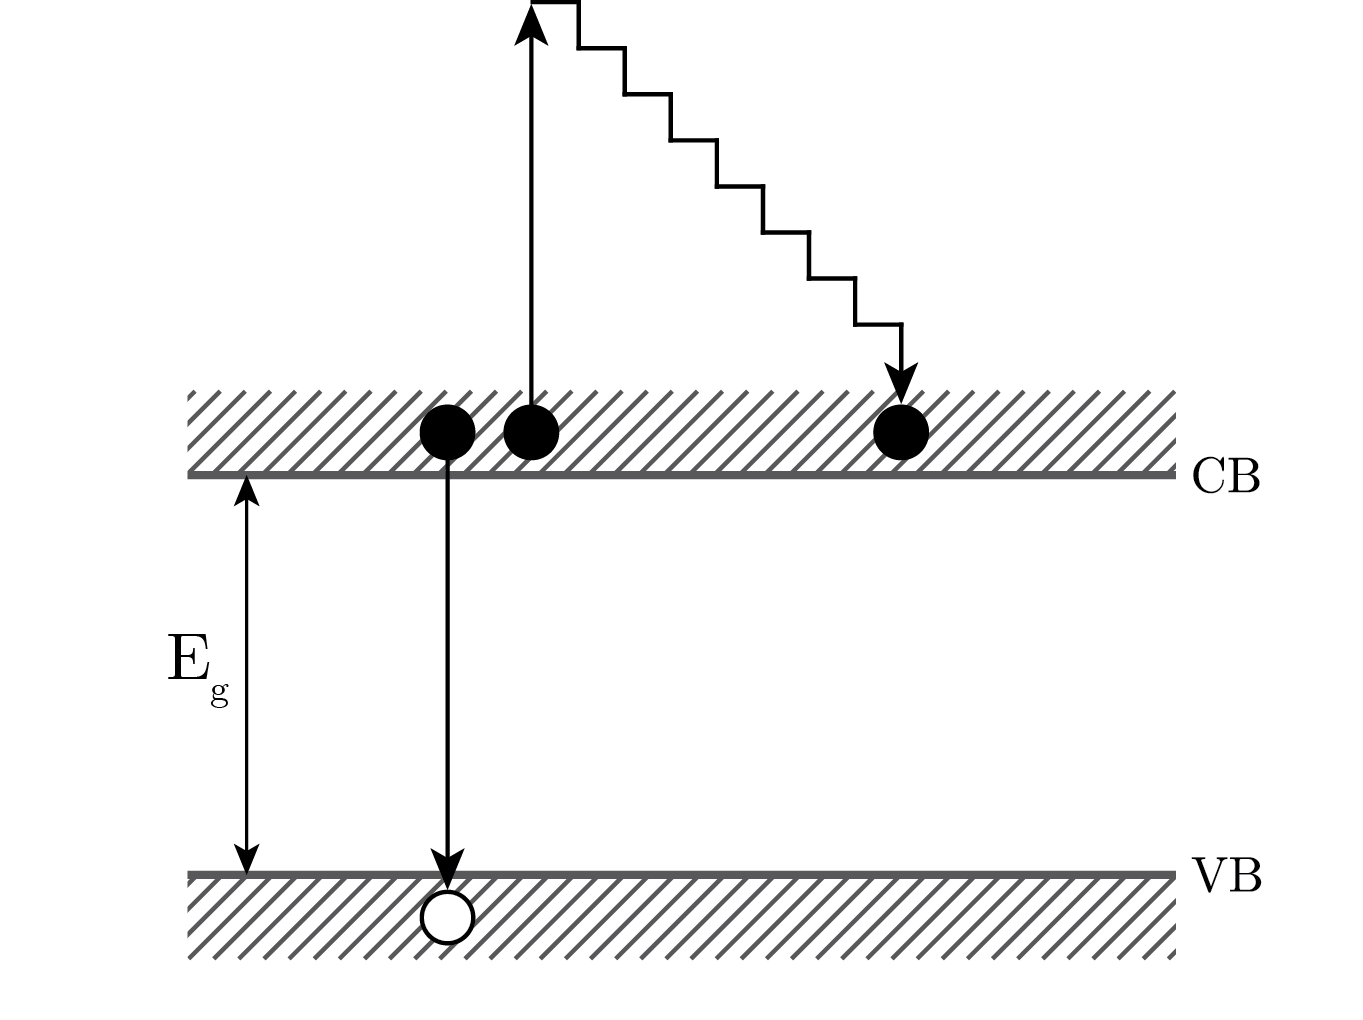
\includegraphics[width=1\linewidth]{\figurepath/slme/AugerRec1.png} 
\caption{} 
\end{subfigure}% 
\begin{subfigure}{0.50\textwidth} 
\centering 
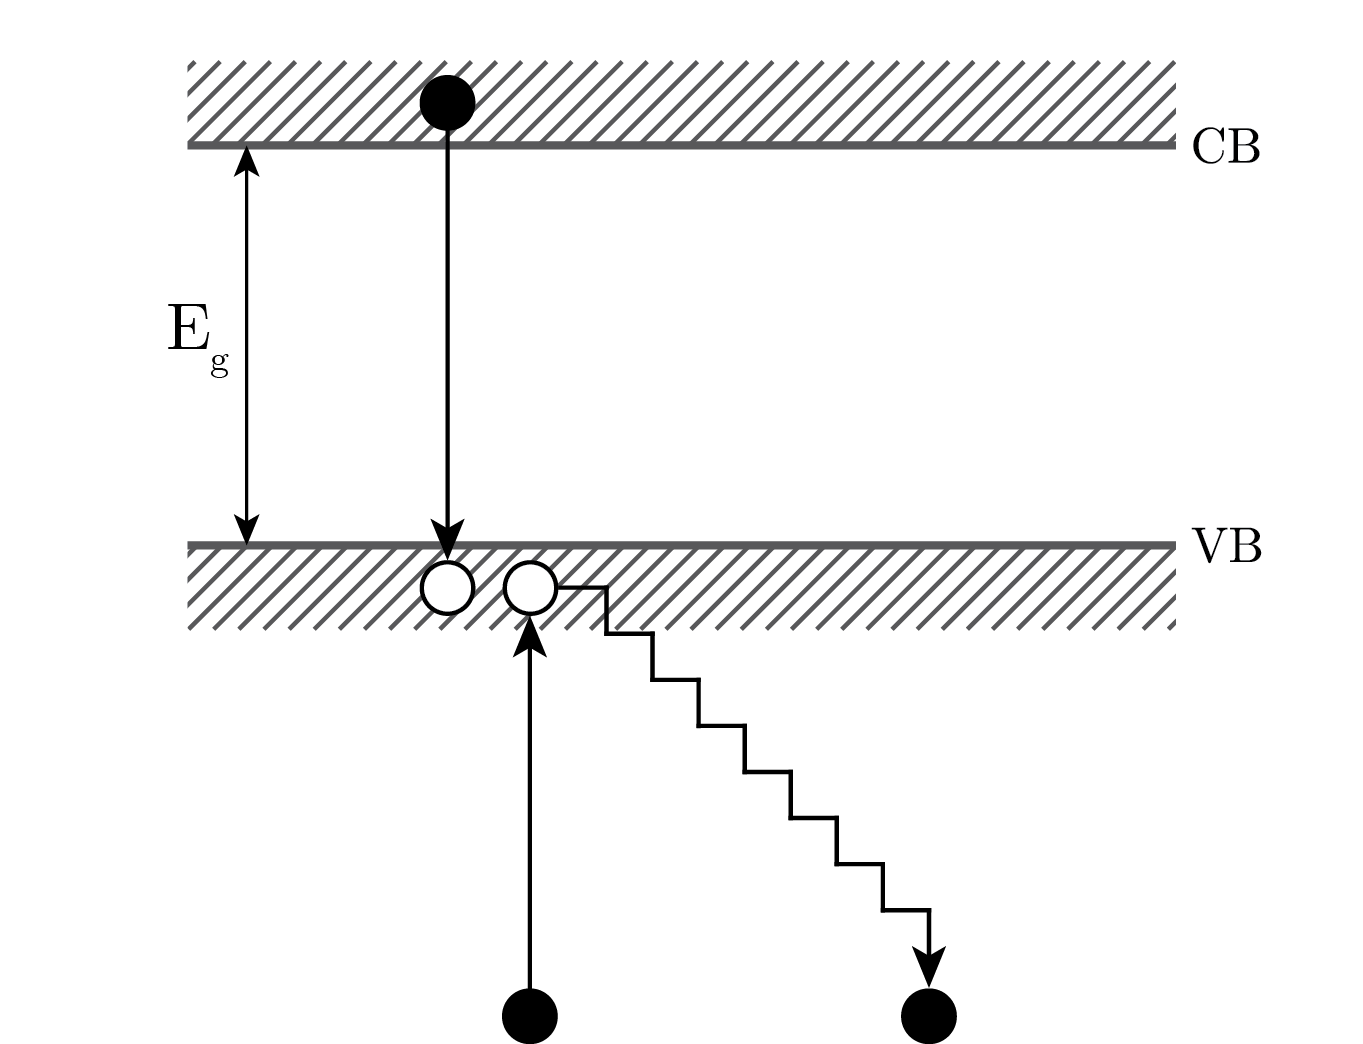
\includegraphics[width=1\linewidth]{\figurepath/slme/AugerRec2.png} 
\caption{} 
\end{subfigure} 
\caption{\label{slme:fig-augerrec}Auger Recombination. The recombination 
energy is either passed to an electron in the conduction band (a) or the 
valence band (b).} 
\end{figure} 

\textbf{Shockley-Read-Hall Recombination} (SRH) or trap-assisted 
recombination~\cite{Shockley1952}\cite{Hall1952}. This mechanism uses energy 
levels in the band gap, usually produced by defects or impurities, in order to 
relax from the conduction band through a two step process. The electron first 
undergoes a transition to the energy level created by the defect, after which 
it recombines with a hole in the valence band~(Fig.~\ref{slme:fig-SRHrec}). 
Since SRH recombination uses energy levels in the band gap which are produced 
by defects, this mechanism is more important in materials which are heavily 
doped. It is also possible to demonstrate that defect levels situated near the 
middle of the band gap are the most effective for the SRH recombination, 
providing larger recombination rates~\cite{Green1981}. 
\begin{figure}[ht]  
\centering 
\includegraphics[width=0.6\textwidth]{\figurepath/slme/SRHrec.png} 
\caption{\label{slme:fig-SRHrec}Shockley-Read-Hall Recombination.} 
\end{figure} 

\subsection{PN - Junction} 
 
When a semiconductor is doped with impurity atoms that have more valence 
electrons, there are more electrons in the conduction band that can contribute 
to the conductivity of the material. This is called a \textit{n-type} 
semiconductor. If atoms are introduced that have less valence electrons, there 
is an increased amount of holes in the valence band, also improving the  
conductivity in what is referred to as a \textit{p-type} semiconductor. By 
joining a n-type and p-type semiconductor, we form what is known as a 
\textit{P-N~junction~diode}~\cite{Shockley1949}~(Fig.~\ref{slme:fig-PNjunction}). 
 
\begin{figure}[ht]
\centering 
\captionsetup{width=0.8\textwidth}
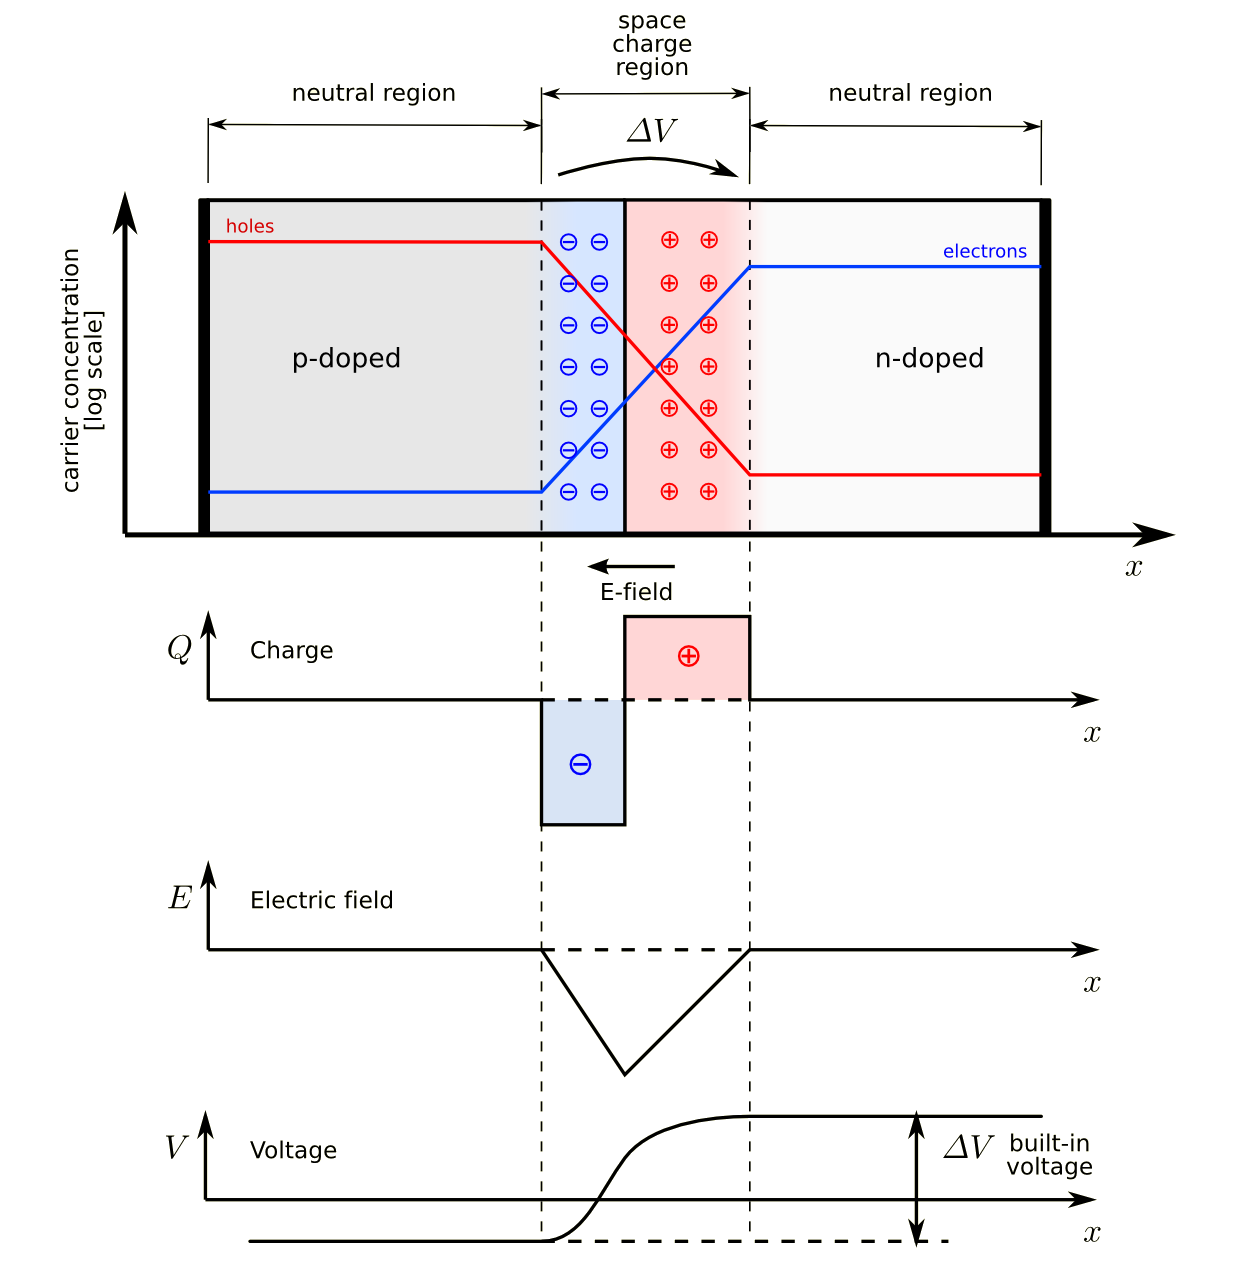
\includegraphics[width=0.9\textwidth]{\figurepath/slme/PN-Junction.png} 
\caption{\label{slme:fig-PNjunction} The P-N Junction. \cite{PNjunction}} 
\end{figure} 
 
An important effect caused by putting these two types of materials together is 
the creation a \textit{depletion region}, which is a result of the electrons 
and holes looking for an equilibrium by moving to the other side of the P-N 
junction. When the electrons move from the n-type to the p-type region, they 
leave behind positively charged ion cores. Similarly, holes moving across the 
junction create a negative surplus charge in the p-type semiconductor. This 
charge imbalance creates an electric field at the center region of the diode, 
which eventually puts a stop to the migration of electrons and holes. The 
result is a potential difference across the P-N junction, which is required to 
separate the charge carriers generated by the absorption of incoming light. 
 
By applying a voltage across the P-N junction, we can influence the strength 
of the electric field in the depletion region. Under \textit{forward bias}, we 
decrease the voltage difference over the diode, making it easier for the 
charge carriers to move across the junction. This has the potential of 
increasing the power output, but also raises the possibility that the 
electrons and holes can recombine. In the \textit{reverse} bias case, the 
magnitude of the electric field across the junction is increased, and the charge carriers are 
more or less confined to their respective regions.  
 
\subsection{Ideal Diode Law} 
 
In order to properly model the functioning of a solar cell, we need to know 
the I-V characteristic of the P-N~junction. If we write down the electron and 
hole densities as $n(x)$ and $p(x)$, along with their respective current 
densities $J$, mobilities $\mu$ and diffusivity constants $D$, the dynamics of 
the electrons and holes in the different regions of the P-N diode can be 
characterized by a set of basic equations~\cite{Shockley1949}: 
\vspace{0.1in} 
\begin{enumerate} 

\item \textbf{Poisson's Equation: } \begin{equation}\frac{\partial 
E_x}{\partial x} = \frac{\rho}{\epsilon},\end{equation} 
 
\item \textbf{Transport Equations: } \begin{equation}J_n = e \mu_n n(x) E_x + 
e D_n\frac{\partial n }{\partial x}, \hspace{0.6in} J_p = e \mu_p p(x) E_x - e 
D_p \frac{\partial p}{\partial x},\end{equation} 
 
\item \textbf{Continuity Equations: } \begin{equation}\frac{\partial 
n}{\partial t} = \frac{1}{e} \frac{\partial J_n}{\partial x} - (U - G), 
\hspace{0.6in} \frac{\partial p}{\partial t} = - \frac{1}{e} \frac{\partial 
J_p}{\partial x} - (U - G),\end{equation} 

\end{enumerate} 
where $E_x$ is the electric field, $\rho$ is the charge density, $\epsilon$ is 
the material permittivity and $e = 1.602\cdot 10^{-19}$ \si{\coulomb} is the standard 
electronic charge. The generation rate $G$ and recombination rate $U$ describe 
the creation and annihilation of electron-hole pairs, and are determined by 
the absorption and recombination processes described in 
Sections~\ref{slme:sec-absorption} and~\ref{slme:sec-recombination}.  
 
These equations can be readily solved using numerical approaches. However, by 
applying a few approximations, it is possible to derive a general relation for 
the I-V characteristic of a P-N~junction under dark conditions, known as the \textit{Ideal Diode 
Law}~\cite{Shockley1949}: 
\begin{equation}\label{slme:eq-idealdiode} 
I = I_0 (e^\frac{e V}{k_B T} - 1), 
\end{equation} 
with $k_B$ Boltzmann's constant and $T$ the temperature of the diode. The 
current $I_0$ in Eq.~\ref{slme:eq-idealdiode} is called the \textit{reverse 
saturation} current, which is a measure of the recombination in the device. In 
light of its connection with recombination effects, $I_0$ is also referred to 
as the recombination current~\cite{Cuevas2014}. 
 
\subsection{Working Principles of a Solar Cell} 
 
We now turn to a basic discussion of the working principles of photovoltaic 
devices~\cite{Fonash2010}. Figure~\ref{slme:fig-solarcell} shows the design of 
a conventional solar cell. The top and base layer usually consist of a n-type 
and p-type doped material, not necessarily derived from the same compound. The 
layers form a P-N junction, which is connected on both sides to electrodes 
that are responsible for extracting the charge carriers from the photovoltaic 
device. In order to prevent losing too much of the incoming light to 
reflection, an \textit{anti-reflective} (AR) coating~\cite{Swatowska2011} is 
applied to the top layer. Many solar cells also use a reflective back surface 
(not shown in figure) to increase the path length of the incoming light 
through the absorber layer. 
 
\begin{figure}[ht]  
\centering 
\captionsetup{width=0.8\textwidth}
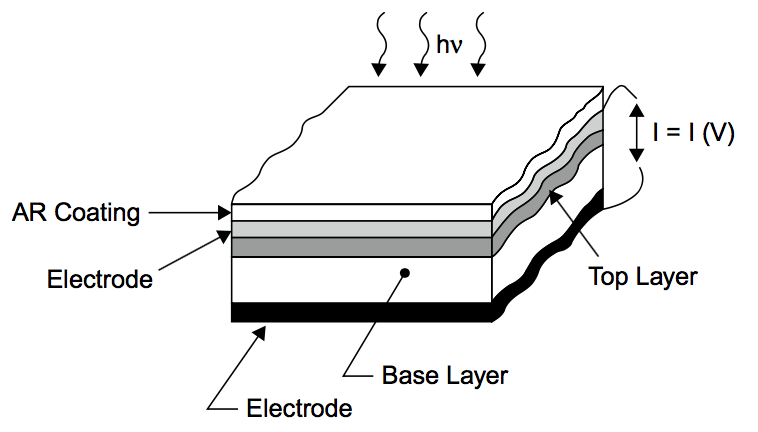
\includegraphics[width=0.8\textwidth]{\figurepath/slme/structure.png} 
\caption{\label{slme:fig-solarcell} Cross section of a typical solar cell. 
Taken from~\cite{Fonash2010}.} 
\end{figure} 

When the absorber layer captures an incoming photon, the material is brought 
into a higher energy state, usually by the creation of an exciton or free 
electron-hole pair. In the case an exciton is produced, it must first be 
dissociated into an electron and a hole. Once the charge carriers are free to 
move, they go to their respective electrode interface. During this stage it is 
crucial that the electron does not recombine with another hole before it is 
extracted from the device. Once the electron reaches the cathode, it makes its 
way to an external load, where it transfers its energy before moving to the 
anode. Finally, the electron reaches the bottom layer and recombines with a 
hole. 

\pagebreak[4]
The process of generating a current from a solar cell can be summarized in 
five steps, which are visualized by drawing an energy band diagram for the 
absorption process in Figure~\ref{slme:fig-working}: 
 
\vspace{0.25in} 
\begin{enumerate}[I.]  
 
\item Transition into an excited state by the absorption of an incoming 
photon.  
 
\item Conversion of the excited state into at least one electron-hole pair. 
 
\item Transport of the charge carriers to their respective electrodes. 
 
\item Transfer of the electron's energy at an exterior load. 
 
\item Recombination of the electron with the hole. 
 
\end{enumerate} 
\vspace{0.50in} 
 
\begin{figure}[ht]  
\centering 
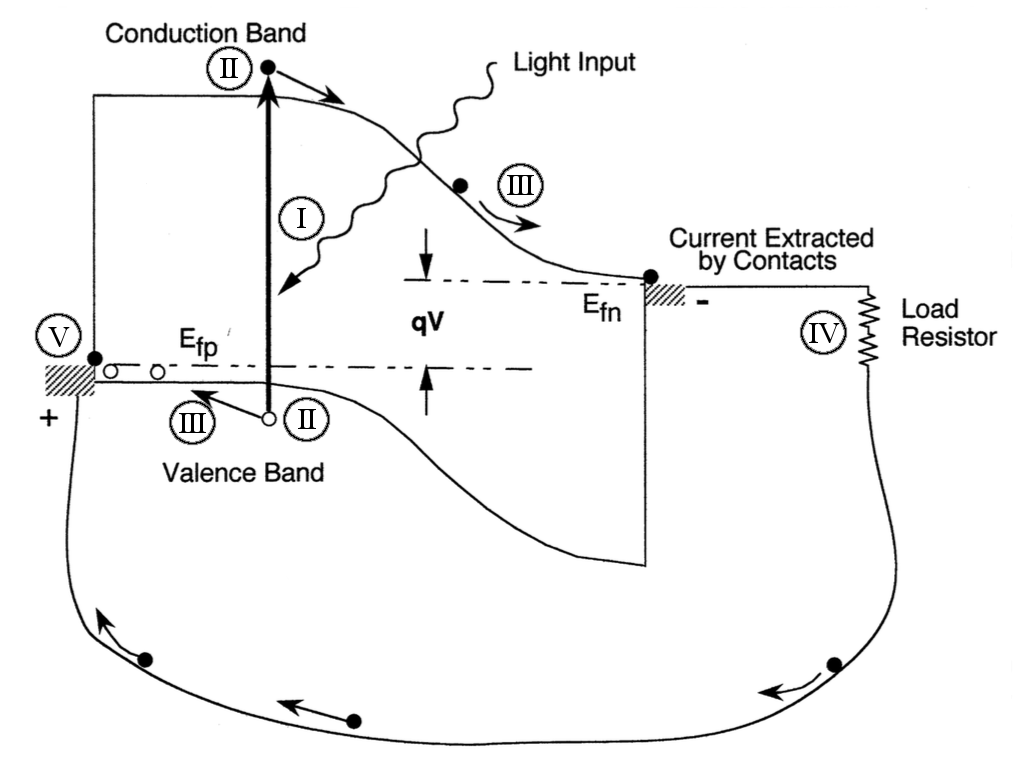
\includegraphics[width=0.9\textwidth]{\figurepath/slme/Working.png} 
\caption{\label{slme:fig-working} Step by step visualisation of the different 
processes in a solar cell. Adapted from \cite{Smestad2002}.} 
\end{figure} 
 
The I-V characteristic of the solar cell under dark conditions is given by the 
ideal diode law~(Eq.~(\ref{slme:eq-idealdiode})). When the solar cell is 
illuminated, the I-V equation becomes\footnote{Note that in principle, the I-V 
curve is given by $I = I_0 (e^\frac{e V}{k_B T} - 1) - I_{sc}$, but the 
convention is to invert the current axis.}~\cite{Lindholm1979}: 
\begin{equation}\label{slme:eq-IV} 
I = I_{sc} - I_0 (e^\frac{e V}{k_B T} - 1), 
\end{equation} 
where $I_{sc}$ is the \textit{short circuit} current. This current is a result 
of the generation of charge carriers due to absorption of incoming photons. In 
many cases, the currents in Eq.~\ref{slme:eq-IV} are expressed as current 
densities\footnote{Note that these current densities are not defined in the 
conventional way. Rather, they are considered as currents per surface area of 
the solar cell. This allows us to ignore the surface area of the solar cell in 
our discussion.} ($J,J_0,J_{sc}$), and I follow the same convention 
throughout this text. Figure~\ref{slme:fig-IV_char}(a) shows the I-V 
characteristic of a solar cell under illuminated and dark conditions, whereas 
Figure~\ref{slme:fig-IV_char}(b) demonstrates the definition of the 
\textit{Fill Factor}~(FF)~\cite{Fonash2010}: 
\begin{equation} 
FF = \frac{P_{m}}{V_{oc} J_{sc}}, 
\end{equation} 
where $P_m = J_m V_m$ is the maximum power density and $V_{oc}$ is the 
\textit{open circuit} voltage, which is the voltage of the diode at $J = 0$: 
\begin{equation} 
J_{sc} - J_0 (e^\frac{eV_{oc}}{k_B T}-1) = 0 \hspace{0.1in} \Leftrightarrow 
\hspace{0.1in} V_{oc} = \frac{k_B T}{q} \ln (\frac{J_{sc}}{J_0} + 1). 
\end{equation} 
The fill factor is a measure for how close a given characteristic is to 
obtaining the ideal power density $J_{sc}V_{oc}$, i.e. operating at the 
short-circuit current and open-circuit voltage. 
 
\begin{figure}[ht]  
\centering 
\captionsetup{width=0.9\textwidth} 
\begin{subfigure}{0.5\textwidth} 
\centering 
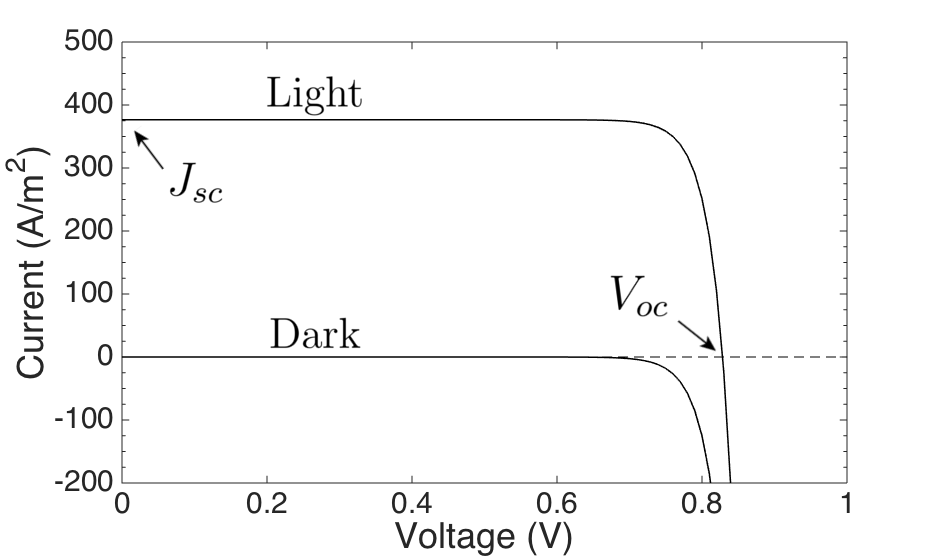
\includegraphics[width=1\linewidth]{\figurepath/slme/IVchar.png} 
\caption{} 
\end{subfigure}% 
\begin{subfigure}{0.5\textwidth} 
\centering 
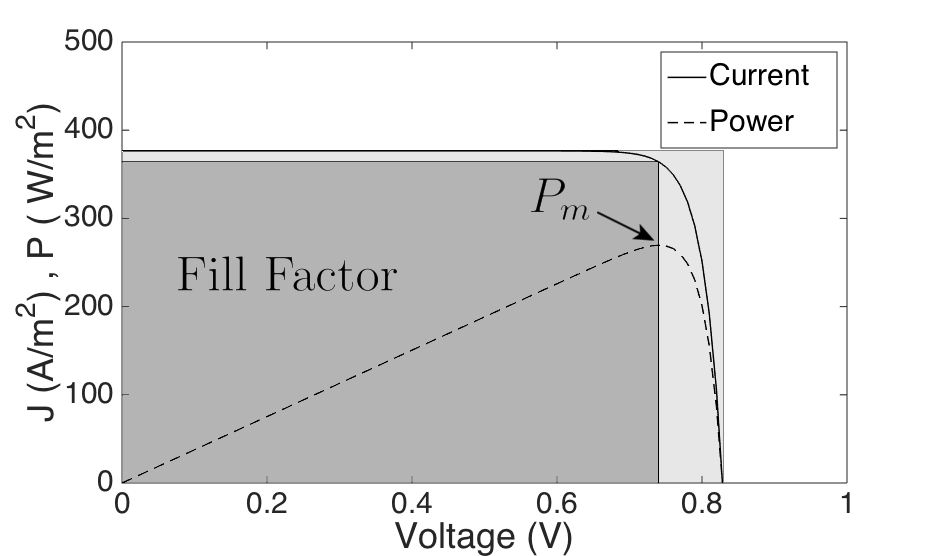
\includegraphics[width=1\linewidth]{\figurepath/slme/FillFactor.png} 
\caption{} 
\end{subfigure} 
\caption{\label{slme:fig-IV_char} (a) I-V curve of a solar cell under dark and 
illuminated (light) conditions. (b) Power maximization and the corresponding 
fill factor, given by the dark area ($P_m$) divided by the light area ($V_{oc} 
J_{sc}$).} 
\end{figure} 

\section{Selection Metric}\label{slme:sec-metric} 
 
Materials play a central role in the effort to produce cheaper and more 
efficient solar cells. The discovery of improved absorber materials has the 
potential to significantly increase the cost-effectiveness of photovoltaic 
devices, but experimental trial and error methods are often slow and 
expensive. Computational high throughput screening can offer a quick and 
relatively cheap approach for refining the selection of materials which warrant 
experimental investigation. In order to do so, however, a suitable selection 
metric is required that can determine the potential of a material to function 
as an absorber layer in a solar cell. 

The \textit{Spectroscopic Limited Maximum Efficiency} (SLME) is a 
calculable selection metric that tries to improve upon its predecessors by 
including the absorption spectrum, calculated from first-principles methods, 
in its estimation of the efficiency of materials as absorber layers. This 
section is dedicated to explaining the SLME metric, as well as its 
predecessor, the Shockley-Queisser (SQ) limit.  
 
\subsection{Solar Cell Efficiency} \label{slme:sec-efficiency} 
 
In order to compare the performance of solar cells, we need to have a gauge 
for their efficiency. A sensible way of defining the efficiency of a 
photovoltaic device is as the ratio of the maximum power density $P_m$ 
produced by the solar cell, and the total incident power density from the 
solar spectrum $P_{in}$~\cite{Fonash2010}: 
\begin{equation} 
\eta = \frac{P_m}{P_{in}}. 
\end{equation} 
When determining the efficiency, it is important to use agreed upon conditions 
for the measurement and calculation of both power densities. For the solar spectrum, 
researchers normalize the AM1.5G spectrum to produce a total incident power 
density of 1 \si{\kilo\watt \per \meter\squared}, and generate it in a lab to find 
experimental values for the output power density of the solar cell. The 
reference temperature of the device is usually 25 \si{\celsius}. 
Figure~\ref{slme:fig-effchart} shows the evolution of the maximum efficiency 
found for different types of solar cells. We can see that the current highest 
performance is achieved by the multi-junction PV devices, which use a 
combination of P-N junctions with a different band gap for each semiconductor 
compound~\cite{Dimroth2007}. The materials are chosen with decreasing band 
gaps, so that the higher energy photons are absorbed first. In this way, the 
multi-junction solar cell absorbs photons over a large range of frequencies, 
and loses less energy to thermic relaxation of electrons in the conduction 
band. Other promising results are shown for the \textit{thin film} 
technologies~\cite{Shah2004}, which focus on reducing the material consumption 
in an attempt to make PV energy generation more financially competitive. 
Finally, there is an increasing interest in developing organic cells, which 
have the potential of being very cost effective and having far less impact on 
the environment. 

\begin{sidewaysfigure}
    \centering
    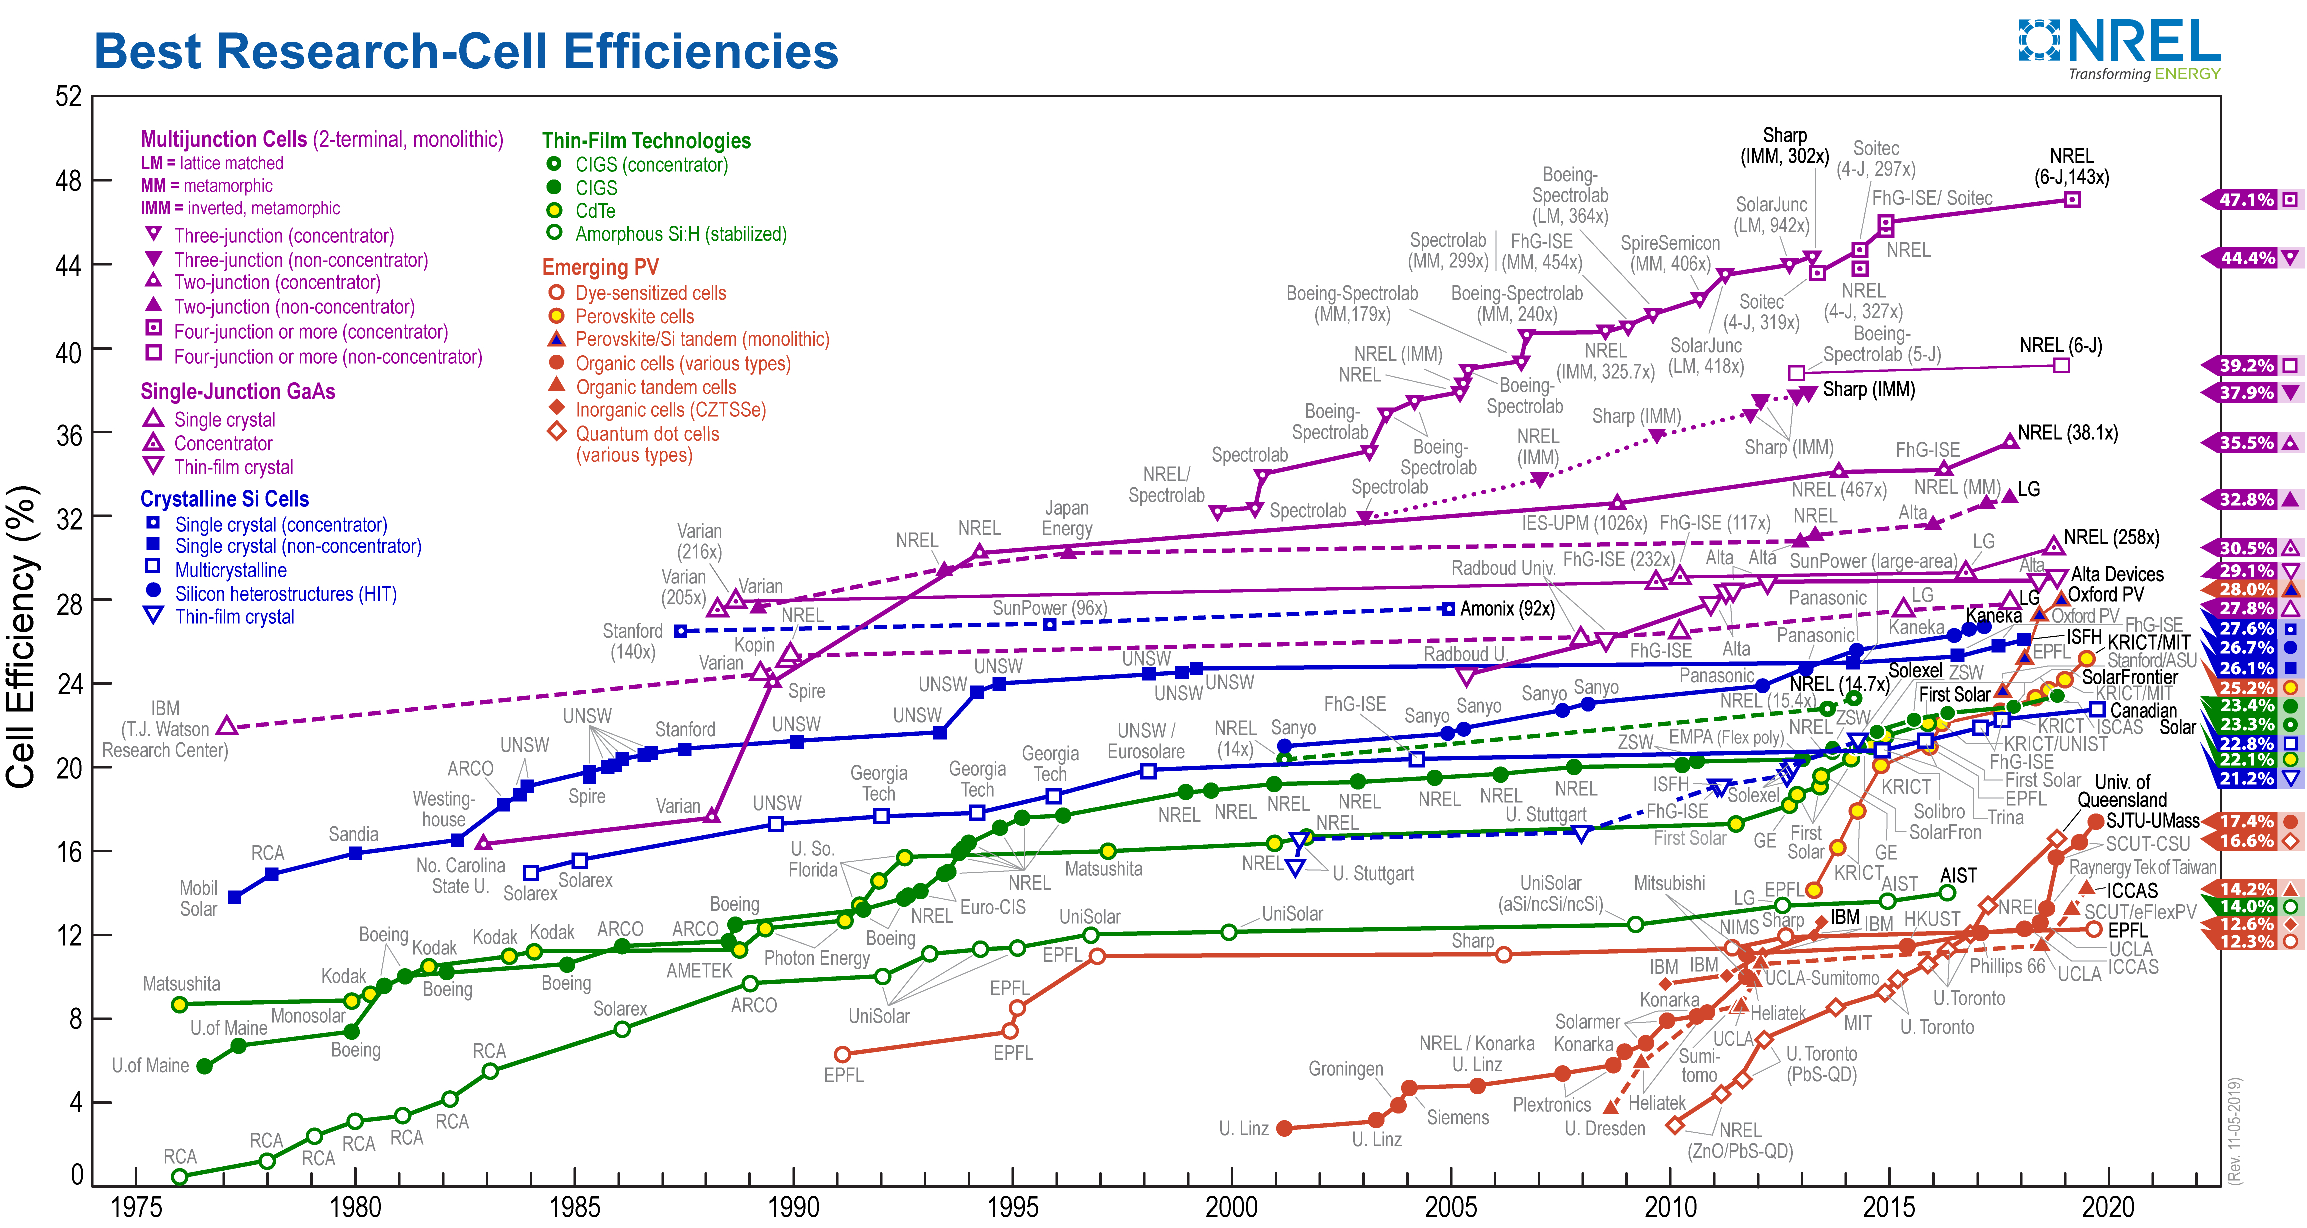
\includegraphics[width=1\textwidth]{\figurepath/slme/efficiency_chart.png} 
    \caption{\label{slme:fig-effchart} Overview of the evolution of solar cell 
efficiencies over the past four decades. Provided by NREL~\cite{NREL2019}.} 
    \label{fig:awesome_image}
\end{sidewaysfigure}

\subsection{Shockley-Queisser Limit} \label{slme:sec-SQlimit} 
 
In 1961, Shockley and Queisser proposed a theoretical upper limit for the 
efficiency of PV devices with a single P-N junction, which solely depends on 
the band gap of the absorber material~\cite{Shockley1961}. Their derivation is 
based on the principle of \textit{detailed balance}, which states 
that~\cite{Klein1955}: ``\textit{transitions between any two states take place 
with equal frequency in either direction at equilibrium}". They also make the 
assumption that every incident photon with an energy above the band gap ($h\nu 
> E_g$), no matter how high its energy, produces a single electron-hole 
pair\footnote{As Shockley and Queisser note in their original paper, it is 
possible to have a higher absorber layer efficiency than the SQ limit, for 
example if we include the possibility that one photon produces multiple 
electron-hole pairs.}. This corresponds to setting the absorptivity $a(E)$ - 
the chance that an incoming photon is captured by the absorber layer - to a 
step function: 
\begin{equation}\label{slme:eq-step_a} 
a(E) =  \begin{cases} 0, & \mbox{if } E < E_g \\ 1, & \mbox{if } E \geq E_g 
\end{cases} 
\end{equation} 
 
To calculate $P_m$, the power density $P = JV$ is maximized versus the voltage 
$V$, where the current density $J$ is derived from the ideal $J-V$ 
characteristic of an illuminated solar cell (Eq.~(\ref{slme:eq-JV})): 
\begin{equation}\label{slme:eq-JV} 
J = J_{sc} - J_0 \left(e^{\frac{eV}{k_B T}} - 1\right). 
\end{equation} 
The short-circuit current density $J_{sc}$, also known as the photogenerated 
current or the illuminated current, is calculated from the number of photons 
of the solar spectrum that are absorbed by the solar cell: 
\begin{align} 
J_{sc} = e &\int_0^{\infty} a(E) \Phi_s (E) dE \\ 
\stackrel{(\ref{slme:eq-step_a})}{=} e &\int_{E_g}^{\infty} \Phi_s (E) dE 
\label{slme:eq-Ish} 
\end{align} 
where $\Phi_s(E)$ is the photon flux density of the solar spectrum. In their 
original paper, Shockley and Queisser used a blackbody spectrum of $T_s = 
6000~\si{\kelvin}$, but the current convention is to use the AM1.5G solar 
spectrum~\cite{International2012}.  The reverse saturation current density 
$J_0$ is calculated by considering the principle of detailed balance, i.e. in 
equilibrium conditions the rate of photon emission from radiative 
recombination must be equal to the photon absorption from the surrounding 
medium. Because the cell is considered to be attached to an ideal heat sink, 
the ambient temperature is the same as that of the solar cell. Hence, the 
spectrum of the surrounding medium is that of a black body at cell temperature 
$T$: 
\begin{align} 
J_0 = e \pi &\int_0^{\infty} a(E) \Phi_{bb}(E) dE\nonumber \\ 
= e \pi &\int_0^{\infty} a(E) \frac{2E^2}{h^3 c^2} \frac{dE}{e^{\frac{E}{k_B 
T}}-1} \\ 
\stackrel{(\ref{slme:eq-step_a})}{=} e \pi &\int_{E_g}^{\infty} 
\frac{2E^2}{h^3 c^2} \frac{dE}{e^{\frac{E}{k_B T}}-1} \label{slme:eq-I0} 
\end{align} 
where $h$ is Planck's constant and $c$ is the speed of light. As mentioned previously, because of its 
connection with the recombination of electron-hole pairs at equilibrium, $J_0$ 
is also referred to as the recombination current density~\cite{Cuevas2014}. 
This is the convention used in the sections that follow. 
 
The resulting function for the efficiency only depends on the band gap $E_g$ 
and is called the Shockley-Queisser or detailed balance limit. 
Figure~\ref{slme:fig-SQlimit} shows the curve for the SQ limit for band gaps 
with an efficiency above 5\%. The maximum conversion of the incoming power 
density is 33.7\%, found for a band gap of 1.34 eV. 
 
\begin{figure}[ht]  
\centering 
\begin{tikzpicture}

\begin{axis}[
width=0.5\textwidth, height=5cm,
tick align=outside,
tick pos=left,
x grid style={white!69.0196078431373!black},
xlabel={\(\displaystyle E_g\) (eV)},
xmin=0.3, xmax=3,
xtick style={color=black},
y grid style={white!69.0196078431373!black},
ylabel={SQ limit (\%)},
ymin=5, ymax=35,
ytick style={color=black}
]
% This file was created by tikzplotlib v0.9.1.
\addplot [semithick, black]
table {%
0.3 5.15033621252289
0.327272727272727 6.3857621313083
0.354545454545455 7.58069000454293
0.381818181818182 8.84976938774914
0.409090909090909 10.2342069399767
0.436363636363636 11.6143300996967
0.463636363636364 13.0445582666888
0.490909090909091 14.4996610004787
0.518181818181818 15.8935992434198
0.545454545454545 17.046283604579
0.572727272727273 18.0812465593071
0.6 19.1033164037573
0.627272727272727 20.2021782335349
0.654545454545455 21.5702715672073
0.681818181818182 23.0016791190268
0.709090909090909 24.1203654348577
0.736363636363636 24.8109807295411
0.763636363636364 25.3828874313141
0.790909090909091 25.8976746602018
0.818181818181818 26.3482102728689
0.845454545454545 27.1427583187501
0.872727272727273 28.236332977223
0.9 29.546345369389
0.927272727272727 30.7221607636115
0.954545454545455 31.257195818536
0.981818181818182 31.5265878190584
1.00909090909091 31.6910495299742
1.03636363636364 31.88528123522
1.06363636363636 32.1121457229202
1.09090909090909 32.7017909247466
1.11818181818182 33.4687056649073
1.14545454545455 33.5808009041944
1.17272727272727 33.5456891849634
1.2 33.4377202385932
1.22727272727273 33.2751658918183
1.25454545454545 33.0764247287324
1.28181818181818 33.0006353101739
1.30909090909091 33.3387392539041
1.33636363636364 33.7730910273573
1.36363636363636 33.7126752663243
1.39090909090909 33.6058083143709
1.41818181818182 33.2439355958915
1.44545454545455 32.8698771916079
1.47272727272727 32.4994619256667
1.5 32.1380650093095
1.52727272727273 31.866594956426
1.55454545454545 31.4180536330263
1.58181818181818 30.9411758377445
1.60909090909091 30.3986802139389
1.63636363636364 30.2671296550965
1.66363636363636 29.7131399733406
1.69090909090909 29.1828331914575
1.71818181818182 28.7540465110178
1.74545454545455 28.2892565465192
1.77272727272727 27.7292365398946
1.8 27.1941948986972
1.82727272727273 26.6429920081977
1.85454545454545 26.0256480282101
1.88181818181818 25.4241814426641
1.90909090909091 24.8458910856901
1.93636363636364 24.2486976706003
1.96363636363636 23.6510704693181
1.99090909090909 23.0845173349765
2.01818181818182 22.4738293198576
2.04545454545455 21.8811100889738
2.07272727272727 21.2974634828468
2.1 20.730541078779
2.12727272727273 20.1391823925613
2.15454545454545 19.564217632189
2.18181818181818 18.9995580144539
2.20909090909091 18.4102736721221
2.23636363636364 17.8459134849454
2.26363636363636 17.2733073810006
2.29090909090909 16.7086104571312
2.31818181818182 16.1352967821963
2.34545454545455 15.5762309885248
2.37272727272727 15.0433366379047
2.4 14.5416459730213
2.42727272727273 13.9921030034755
2.45454545454545 13.4520344387528
2.48181818181818 12.9400753516931
2.50909090909091 12.3865193508364
2.53636363636364 11.8712889239132
2.56363636363636 11.3942116031346
2.59090909090909 10.8636173905151
2.61818181818182 10.3282031616909
2.64545454545455 9.83037422454624
2.67272727272727 9.3415491072395
2.7 8.82731533877496
2.72727272727273 8.34233927201641
2.75454545454545 7.86984876595518
2.78181818181818 7.42202436924299
2.80909090909091 6.98242889552628
2.83636363636364 6.61171863844352
2.86363636363636 6.24867347347324
2.89090909090909 5.96618681163763
2.91818181818182 5.62380942002777
2.94545454545455 5.28056948832473
2.97272727272727 4.95464941576384
3 4.62132753524128
};

\end{axis}

\end{tikzpicture}

\caption{\label{slme:fig-SQlimit} The Shockley-Queisser limit, based on the 
AM1.5G spectrum.} 
\end{figure} 
 
\subsection{Spectroscopic Limited Maximum Efficiency} \label{slme:sec-SLME} 
 
Although the work of Shockley and Queisser was an important step forward, only 
relying on the band gap as the only piece of information to determine the 
efficiency of a compound is too limited. Modern quantum mechanical models 
allow us to determine the response of a material to an incident photon in much 
more detail, based on first-principles calculations. The 
spectroscopic limited maximum efficiency (SLME), introduced by Yu and 
Zunger~\cite{Yu2012}, attempts to use these advances in computational materials science 
to get a better picture of which semiconductors have the greatest potential as 
absorber materials. The SLME also includes the thickness of the absorber layer 
in the calculation of the maximum efficiency, and is therefore particularly 
suited to study the thin-film technologies presented in 
Figure~\ref{slme:fig-effchart}. Since its conception, the SLME has been 
successfully applied to perovskites~\cite{Yin2014, Yin2015, Yin2015b, 
Meng2016}, chalcogenides~\cite{Hong2016, Sarmadian2016}, direct band gap 
silicon crystals~\cite{Lee2014, Oh2015} and other materials~\cite{Yu2012b, 
Yokoyama2013, Heo2014, Huang2015}.  

The SLME tries to improve upon the Shockley-Queisser limit in two ways:  
\vspace{0.1in} 
\begin{enumerate}[I.] 
 
\item Instead of assuming that every photon with an energy greater than the 
band gap is absorbed with absolute certainty, the SLME incorporates the 
absorption coefficient $\alpha(E)$ (Sec.~\ref{slme:sec-absorption}) of the 
material in order to more accurately model the generation of electron-hole 
pairs. After calculating the absorption coefficient from first-principles, it is 
included in both the calculation of the short circuit current and the 
recombination current. This is done through the \textit{absorptivity} $a(E)$, 
which is defined as the fraction of sunlight that is absorbed when the photons 
pass twice through a layer of thickness $L$: 
\begin{equation} \label{slme:eq-absorptivity} 
a(E) = 1 - e^{-2 \alpha(E) L}. 
\end{equation} 
 
\item Similar to the SQ limit, the SLME models radiative recombination using the absorptivity in 
combination with the black-body spectrum at the temperature $T$ of the device. 
In order to include the non-radiative recombination mechanisms, Yu and Zunger 
make the following consideration. The total recombination current is the 
sum of the radiative and non-radiative parts $J_0 = J_0^r + J_0^{nr}$. If one 
defines $f_r$ as the fraction of radiative recombination\footnote{Actually, 
Shockley and Queisser also considered the fraction of radiative recombination 
in their original paper~\cite{Shockley1961}. They did not, however, provide a model to calculate it, 
simply observing that the maximum efficiency is significantly reduced for 
small fractions $f_r$.}, the total recombination current density can be 
written as: 
\begin{equation} 
J_0^r = f_r J_0 \hspace{0.1in} \Leftrightarrow \hspace{0.1in} J_0 = 
\frac{J_0^r}{f_r}. 
\end{equation} 
The fraction of radiative recombination is expressed as a Boltzmann factor:  
\begin{equation} \label{slme:eq-fraction} 
f_r = e^{-\frac{\Delta}{kT}}, 
\end{equation} 
where $\Delta$ is the difference in energy between the direct allowed and 
fundamental band gap: $\Delta = E_g^{da} - E_g$. Using this approximation, the 
recombination of direct band gap absorber materials is entirely radiative in 
nature ($f_r = 1$). However, for indirect band gap semiconductors ($\Delta 
\neq 0$), the non-radiative recombination quickly becomes the dominant 
mechanism. This is in accordance with what is observed experimentally for 
direct and indirect band gap semiconductors. 
\end{enumerate} 
\vspace{0.1in} 
 
The process for determining the SLME is schematically presented in 
Figure~\ref{slme:fig-SLMEcalc}. First, the absorptivity is computed from the 
absorption coefficient, derived from \textit{ab initio} calculations. 
The absorptivity is then used to determine the short 
circuit and radiative recombination current densities: 
\begin{equation} \label{slme:eq-currents} 
\begin{aligned} 
J_{sc} &= e \int_0^\infty a(E)  \Phi_{s} (E) dE, 
\\ J_0^r &= e\pi \int_0^\infty a(E)  \Phi_{bb} (E,T) dE, 
\end{aligned} 
\end{equation} 
where $\Phi_{s}(E)$ and $\Phi_{bb}(E,T)$ are once again the solar spectrum AM1.5G  
and the black-body spectrum at device temperature $T$. The optical 
and fundamental band gaps, also retrieved from first-principles calculations, 
are then used to derive the radiative fraction $f_r$ (Eq.~(\ref{slme:eq-fraction})). From 
here, it is a simple matter of dividing $J_0^r$ by $f_r$ to find the total 
recombination current density $J_0$. Once both $J_{sc}$ and $J_0$ have been determined, the $J$-$V$ characteristic of the illuminated P-N junction 
(Eq.~(\ref{slme:eq-JV})) is used to calculate the total current density versus a range 
of voltages $V$ up to the open circuit voltage $V_{oc}$. Finally,  
the product $J\cdot V$ is maximized versus $V$ to find the maximum output power density 
$P_m$. The SLME efficiency is the result of $P_m$ divided by the total 
incident power density $P_{in}$ = 1 kW/m$^2$. 
 
 
\begin{figure}[ht]  
\centering 
\definecolor{grey900}{HTML}{1F2832}

\tikzstyle{calcbox} = [
draw, color=grey900, thick,
rounded corners, 
inner sep=5,
font=\sffamily\sansmath
]
\tikzstyle{calcarrow} = [
color=grey900, thick,
->, >=latex
]

\begin{tikzpicture}

%% NODES

\node (ab_initio) [calcbox] at (0, 0) {\textit{ab initio}};

% Left branch

\node (alpha) [calcbox, left=3em of ab_initio] {$\alpha(E)$};
\node (abs) [calcbox, below=1em of alpha] {%
$\displaystyle a(E) = 1 - e^{-2\alpha(E)L}$
};

\node (Jsc) [calcbox, below=1em of abs, text width=14em, align=center] {%
$\displaystyle J_{sc} = e \int_0^{\infty} a(E) \Phi_{sun}(E) dE $
};
\node (J0r) [calcbox, below=-0.04em of Jsc, text width=14em, align=center] {%
$\displaystyle J_0^r = e \pi \int_0^{\infty} a(E) \Phi_{bb}(E) dE $
};

% Right branch
\node (bandgaps) [calcbox, right=3em of ab_initio] {$E_g$, $E_g^{da}$};
\node (fr) [calcbox, below=4em of bandgaps] {$f_r = e^{-\frac{E_g^{da} - E_g}{kT}}$};

% Merge
\node (J0) [calcbox, below right=2em and 1em of J0r] {%
$\displaystyle J_0 = \frac{J_0^r}{f_r}$
};
\node (J) [calcbox, anchor=west] at (J0r.west |- J0) {%
$\displaystyle J = J_{sc} - J_0 \left(e^{\frac{eV}{k_B T}} - 1\right)$
};
\node (efficiency) [calcbox, below=2em of J0] {
$\displaystyle \eta = \frac{P_m}{P_{in}}$
};

%% PATHS

\draw [calcarrow] (ab_initio) -- (alpha);
\draw [calcarrow] (alpha) -- (abs);
\draw [calcarrow] (abs) -- (Jsc);
\coordinate (coord0) at ($(Jsc.west) - (1em, 0)$);
\draw [calcarrow] (Jsc.west) -- (coord0) -- (coord0 |- J) -- (J.west);
\draw [calcarrow] (J0r.east) -- (J0r -| J0) -- (J0.north);

\draw [calcarrow] (ab_initio) -- (bandgaps);
\draw [calcarrow] (bandgaps) -- (fr);
\draw [calcarrow] (fr) -- (fr |- J0) -- (J0.east);

\coordinate (coord9) at ($(J.south) - (2em, 0)$);
\draw [calcarrow] (coord9) -- (coord9 |- efficiency.west) -- node[above, midway, font=\sansmath] {$\displaystyle P_m = \max_V (J\cdot V)$} (efficiency.west);

\end{tikzpicture}

\caption{Schematical representation of the calculation of the SLME metric.} 
\label{slme:fig-SLMEcalc} 
\end{figure} 
 
\section{CuAu-likes} \label{slme:sec-CuAu} 
 
Ternary I-III-VI$_2$ semiconductors, such as the well known 
\ce{Cu(In,Ga)(S,Se)2} compounds, are commonly used as absorber materials to 
produce highly flexible and lightweight solar cells. The high absorption 
coefficient of these compounds allows for cost-efficient absorber layers that 
are particularly suited for deposition on flexible 
substrates~\cite{Reinhard2013}. Laboratory values for the efficiency of 
CuIn(S,Se)$_2$ thin film solar cells have recently reached a record value of 
22.3\%. Furthermore, CuIn(S,Se)$_2$ is also considered a suitable material for 
the top cell in tandem structures~\cite{Cheek2013} and quantum dot based 
luminescent solar concentrators~\cite{Hu2015}. The rapid succession of new 
record efficiencies indicates that there is still room for improvement in 
these applications. 
 
The most common phase of I-III-VI$_2$ class materials is chalcopyrite (CH). When 
growing films of these compounds, however, they are often found to contain 
CuAu-like (CA) domains, a metastable phase of chalcopyrite~\cite{Su1999}. Moreover, it has been 
reported that for CuInS$_2$, the presence of the CuAu-like phase improves the 
short circuit current of the chalcopyrite-based photovoltaic cell. In this 
section I present a first-principles investigation of the efficiency of the CA 
phase for a selection of compounds. Section~\ref{slme:sec-structure} presents 
the structure of the CH and CA phases, as well as an analysis of the thermodynamic 
stability of CH versus CA, in order to determine the likelihood of the presence of CA domains 
within a CH-based solar cell. Section~\ref{slme:sec-CuAu_efficiency} continues by presenting the optoelectronic 
properties of the CA phase materials. Finally, these results are used to calculate 
the SLME and the section consludes with a discussion the obtained efficiencies of specific compounds.  
 
\resultsubsection{Structure and formation energy \label{slme:sec-structure}}{https://github.com/mbercx/phd-thesis/blob/master/jupyter/slme/README.md\#structure-and-formation-energy}{solar_structure} 
 
I-III-VI$_2$ compounds are stable at room temperature in the chalcopyrite (CH) 
structure (space group I$\bar{4}$2d). However, Su and Wei~\cite{Su1999} have 
demonstrated the presence of CuAu-like (CA) orderings (space group 
P$\bar{4}$2m) in thin films of CuIn(S,Se)$_2$, grown by vapor-phase epitaxy on 
Si and GaAs substrates.  Alvarez et al.~\cite{Alvarez2002} also analyzed films 
of CuInS$_2$, using XRD to estimate the relative amount of phase domains. They 
found that the total amount of CA ordered phase in samples grown under Cu-poor 
conditions was between 8\% and 25\%. By growing films of CuInS$_2$ on various 
Si substrates, Su et al.~\cite{Su2000} discovered that although the CA phase 
is always present, the amount of CA domains is influenced by the substrate 
orientation. Moreover, Hahn et al.~\cite{Hahn2001} found that by using a 
Si(001) substrate, the CA phase will dominate the orderings of the cation 
sublattice. Recently, Moreau et al.~\cite{Moreau2015} have stated that for the 
CuInS$_2$ compound, introducing domains of CA phase can lead to a reduction of 
strain in the absorber layer, resulting in an increased carrier mobility and 
reduced recombination. Despite the fact that this phase is often found 
together with CH in thin films, little research has been done to determine its 
properties. Figure~\ref{slme:fig-CuAu_structure} shows the CH and CA structure 
of the ternary I-III-VI$_2$ materials. 
 
\begin{figure}[ht]  
\setlength{\captionmargin}{10pt} 
\centering 
\begin{subfigure}{0.24\textwidth} 
\centering 
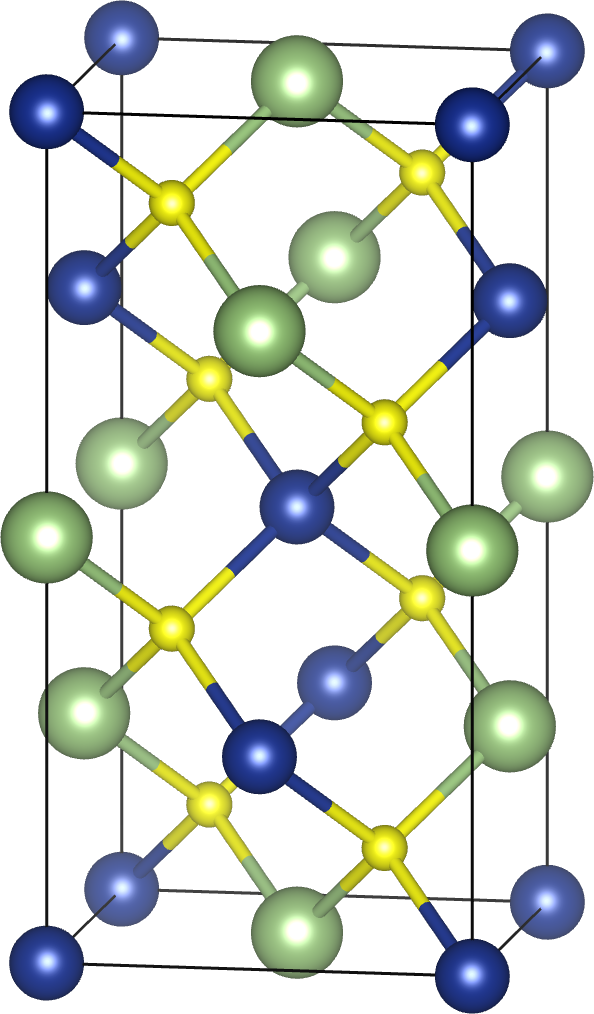
\includegraphics[width=0.8\linewidth]{\figurepath/slme/structures_1.png} 
\caption{} 
\end{subfigure}% 
\begin{subfigure}{0.24\textwidth} 
\centering 
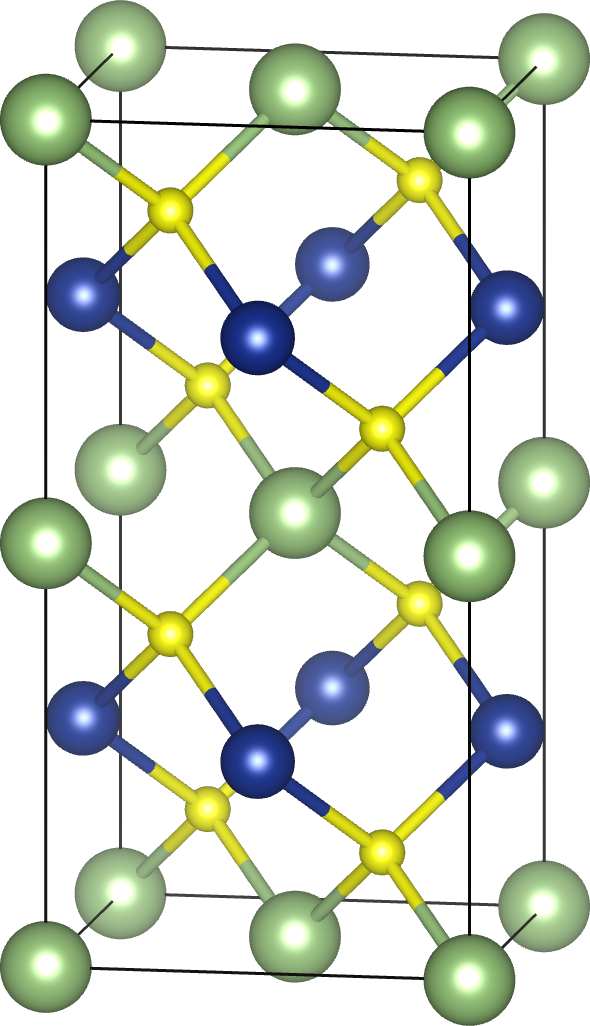
\includegraphics[width=0.8\linewidth]{\figurepath/slme/structures_2.png} 
\caption{} 
\end{subfigure} 
\vspace{0.7em}\\ 
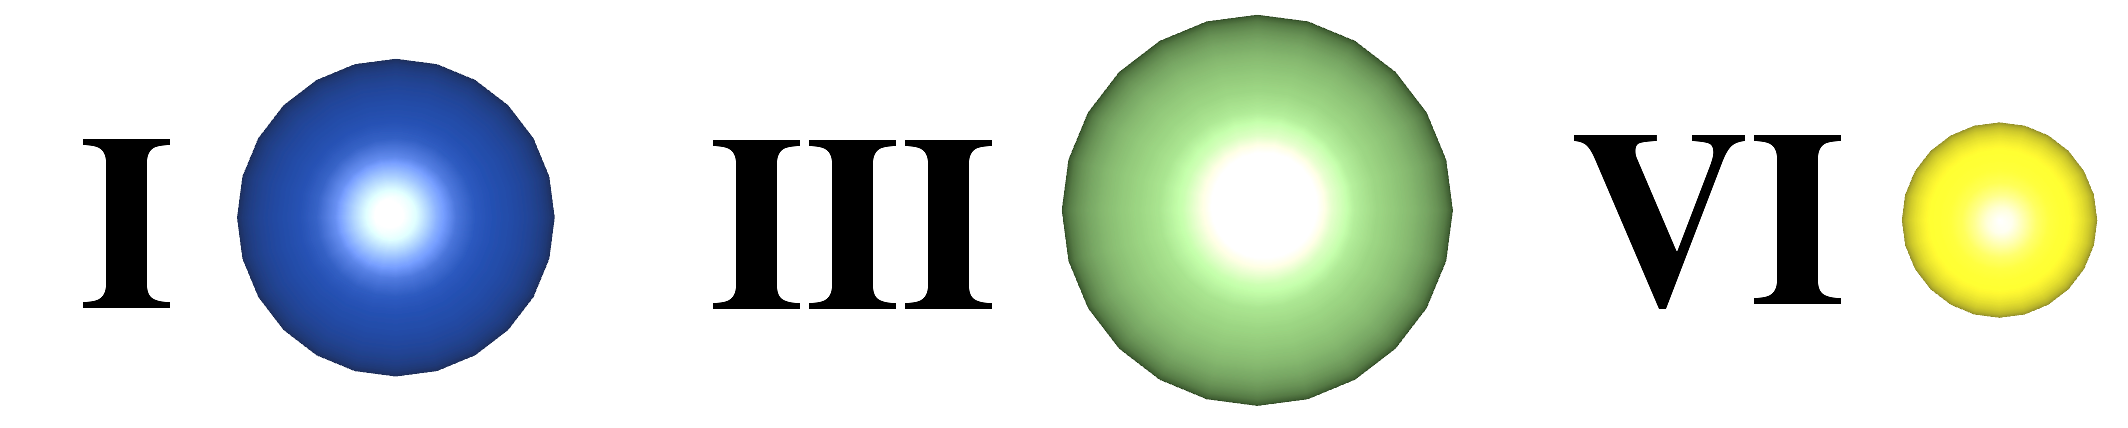
\includegraphics[height=1.8em]{\figurepath/slme/structures_3.png} 
\caption{\label{slme:fig-CuAu_structure} Chalcopyrite (a) and CuAu-like (b) 
structure of ternary \mbox{I-III-VI$_2$} compounds.} 
\end{figure} 
 
\begin{table}[ht] 
\centering 
\renewcommand{\arraystretch}{1.2} 
\caption{Calculated lattice parameters of the \mbox{CuAu-like} (CA) and chalcopyrite (CH) 
phase of the considered compounds, compared with the experimental results from Hahn et al.~\cite{Hahn1953}.} 
\label{slme:tab-lattice} 
\begin{tabular*}{\textwidth}{@{\extracolsep{\fill}}lccccccccc}\hline 
\multirow{2}{*}{Material}    & & CA & & & CH & & & CH (Ref~\cite{Hahn1953}) & 
\\ \cmidrule(lr){2-4} \cmidrule(lr){5-7} \cmidrule(lr){8-10} 
 			&  $a$ (\si{\angstrom}) & $c$ (\si{\angstrom}) & $c/a$ & $a$ 
(\si{\angstrom}) & $c$ (\si{\angstrom}) & $c/a$ & $a$ (\si{\angstrom}) & $c$ 
(\si{\angstrom}) & $c/a$ \\\hline 
AgGaSe$_2$ 	& 5.702 & 12.663 & 2.221 & 6.045 & 11.267 & 1.864 & 5.973 & 10.88 
& 1.823 \\ 
AgGaTe$_2$ 	& 6.220 & 13.060 & 2.100 & 6.403 & 12.327 & 1.925 & 6.283 & 11.94 
& 1.897 \\ 
AgInS$_2$  	& 5.780 & 12.132 & 2.100 & 5.925 & 11.554 & 1.950 & 5.816 & 11.17 
& 1.920 \\ 
AgInTe$_2$ 	& 6.511 & 13.224 & 2.031 & 6.570 & 13.000 & 1.979 & 6.406 & 12.56 
& 1.962 \\ 
CuGaS$_2$  	& 5.341 & 10.861 & 2.033 & 5.384 & 10.669 & 1.982 & 5.349 & 10.47 
& 1.958 \\ 
CuGaSe$_2$ 	& 5.662 & 11.436 & 2.020 & 5.683 & 11.277 & 1.984 & 5.607 & 10.99 
& 1.960 \\ 
CuGaTe$_2$ 	& 6.109 & 12.170 & 1.992 & 6.091 & 12.160 & 1.996 & 5.994 & 11.91 
& 1.987 \\ 
CuInS$_2$ 	& 5.636 & 11.129 & 1.975 & 5.598 & 11.274 & 2.014 & 5.517 & 11.06 & 
2.005 \\ 
CuInSe$_2$ 	& 5.914 & 11.710 & 1.980 & 5.881 & 11.840 & 2.013 & 5.773 & 11.55 
& 2.001 \\ 
CuInTe$_2$ 	& 6.323 & 12.590 & 1.991 & 6.313 & 12.681 & 2.009 & 6.167 & 12.34 
& 2.000 \\ \hline 
\end{tabular*} 
\end{table} 

To estimate the likelihood of finding a significant amount of CA domains in 
CuInSe$_2$, Wei et al.~\cite{Wei1999} used first-principles calculations to 
determine the difference in formation energy $\Delta E_f = E_{tot}^{CA} - 
E_{tot}^{CH}$ between the CH and CA phases of the compound. They found a very 
small energy difference of 2~\si{\milli\electronvolt}/atom, which led them to 
predict the coexistence of the CH and CA structures in CuInSe$_2$. This was 
confirmed experimentally by Su and Wei~\cite{Su1999}, supporting the idea that 
the presence of CA domains is a result of bulk thermodynamics. In order to 
determine the formation energy difference, we first optimize the structure of 
the CA and CH phase for each compound. 
 
Table~\ref{slme:tab-lattice} presents the calculated lattice parameters and 
$c/a$ ratio, as well as the corresponding experimental values 
for the CH phase of the compounds\footnote[3]{No experimental values were 
found for the CA phase in the literature.}. We can see that the calculated 
$c/a$ ratios match well with those obtained from experiment, with a slight overestimation of the calculated results compared to experiment. For the CA phase, 
replacing the cations Ag by Cu or Ga by In decreases the $c/a$ ratio of the 
unit cell. This trend is reversed for the CH phase. Comparing the $c/a$ 
ratio of the CA and CH phase, we find a large difference in the $c/a$ ratio 
for the \mbox{\ce{AgGa-VI2}} compounds. Next, Table~\ref{slme:tab-formation} 
presents the difference in formation energy for the selected list of 
compounds. Our first-principles results for \ce{CuInS2}, \ce{CuInSe2} and 
\ce{CuGaSe2} correspond within 1~\si{\milli\electronvolt} with those of Su et al.~\cite{Su1999}. Similar to 
the results for the $c/a$ ratio, the choice of cations has a large influence 
on the difference in formation energy. From Table~\ref{slme:tab-formation}, it is 
clear that substituting either In by Ga or Cu by Ag increases the difference 
in formation energy of the two phases. This means that if we consider the 
existence of the CA phase to be controlled by bulk thermodynamics, we expect 
CA domains to be common in the \mbox{\ce{CuIn-VI2}} compounds, and less likely 
in the \mbox{\ce{AgGa-VI2}} ones.  

\begin{table}[ht] 
\centering
\sffamily
\captionsetup{width=0.8\textwidth}
\renewcommand{\arraystretch}{1.1} 
\caption{\label{slme:tab-formation} Difference in formation energy between the 
chalcopyrite and CuAu-like structure of the considered ternary I-III-VI$_2$ 
compounds. All energy differences are expressed in \si{\milli\electronvolt}/atom. The results of Su et al.~\cite{Su1999} for \ce{CuInS2}, \ce{CuInSe2} and \ce{CuGaSe2} are also tabulated for comparison.}
\begin{tabular}{ l @{\hskip 2 em} S[table-format=1.1] @{\hskip 2 em} c}
Material & {$\Delta E_f$} & {$\Delta E_f$}~\cite{Su1999} \\\hline 
AgGaSe$_2$ & 31.3 & - \\
AgGaTe$_2$ & 27.8 & - \\
AgInS$_2$ & 8.9 & - \\
AgInTe$_2$ & 8.5 & - \\
CuGaS$_2$ & 8.8 & - \\
CuGaSe$_2$ & 9.9 & 9 \\
CuGaTe$_2$ & 7.0 & - \\
CuInS$_2$ & 1.6 & 2 \\
CuInSe$_2$ & 2.2 & 2 \\
CuInTe$_2$ & 2.9 & - \\\hline 
\end{tabular} 
\end{table} 

\resultsubsection{Absorber layer efficiency \label{slme:sec-CuAu_efficiency}}{https://github.com/mbercx/phd-thesis/blob/master/jupyter/slme/README.md\#absorber-layer-efficiency}{solar_efficiency} 
 
For all of the investigated compounds, we find a direct band gap at the 
$\Gamma$-point. Table~\ref{slme:tab-Eg} presents a comparison between the 
G$_0$W$_0$@HSE06 band gaps calculated for the CA and CH 
structures\footnote[4]{We did not take all of the CH phase band gaps from Yu 
and Zunger~\cite{Yu2012}, because of inconsistencies between the tabulated and 
plotted values for some compounds in this paper.}. The 
G$_0$W$_0$ calculated band gaps for the CA phase are lower than those of the 
CH phase for all compounds besides \ce{CuInS2}. Furthermore, the difference is 
smaller for the \mbox{I-III-S$_2$} structures compared to the 
\mbox{I-III-(Se,Te)$_2$} compounds. Table~\ref{slme:tab-Eg} also contains the 
experimental band gaps of the CH phase of the compounds.  
Although the G$_0$W$_0$@HSE06 band gaps correspond quite well to the 
experimental values for some compounds, there are clear discrepancies for 
others. This could be a result of the sensitivity of chalcogenide band gaps to 
the anion displacement $u$~\cite{Jaffe1983}. As an example of the dielectric function, we show 
the result for \mbox{CA-CuInSe$_2$} in Fig.~\ref{slme:fig-diel_CuInSe2}. The 
results for the other compounds can be found in the 
\href{https://github.com/mbercx/phd-thesis/tree/master/jupyter/slme\#absorber-layer-efficiency}{Jupyter notebooks corresponding to this section}. 

\begin{figure}[ht] 
\centering 
\captionsetup{width=0.8\textwidth}
\begin{tikzpicture}[]

\begin{groupplot}[
group style={group size=1 by 2, vertical sep=1em},
height=4cm,
width=10cm,
xmin=0, xmax=20,
legend style={
at={(0.95, 0.9)}, anchor=north east, font=\small\sffamily, draw=none
},
]

\nextgroupplot[
% xticklabel pos=right,
xlabel={},
xticklabels={},
ylabel={$\varepsilon^{(1)}$},
]
% This file was created by tikzplotlib v0.9.1.
\addplot [semithick, black]
table {%
0 7.2469
0.1127 7.2546
0.2253 7.2784
0.338 7.3198
0.4506 7.3819
0.5633 7.471
0.6759 7.6008
0.7886 7.8133
0.9013 8.0841
1.0139 8.324
1.1266 8.4499
1.2392 8.2965
1.3519 7.8815
1.4645 7.5632
1.5772 7.4722
1.6899 7.4797
1.8025 7.5661
1.9152 7.6914
2.0278 7.8395
2.1405 8.0047
2.2532 8.0767
2.3658 8.1033
2.4785 8.0652
2.5911 8.183
2.7038 7.9324
2.8164 7.3974
2.9291 6.8107
3.0418 6.5668
3.1544 6.6864
3.2671 6.9085
3.3797 7.0628
3.4924 7.238
3.605 7.4287
3.7177 7.4122
3.8304 7.7912
3.943 8.1671
4.0557 8.2489
4.1683 8.4721
4.281 8.4669
4.3936 8.3707
4.5063 7.7924
4.619 7.0775
4.7316 7.4907
4.8443 7.4275
4.9569 6.91
5.0696 6.8821
5.1822 6.1413
5.2949 5.5615
5.4076 4.7508
5.5202 3.9118
5.6329 4.0834
5.7455 3.5859
5.8582 3.9037
5.9708 4.626
6.0835 3.7991
6.1962 3.6056
6.3088 3.5415
6.4215 2.934
6.5341 2.5389
6.6468 1.0614
6.7595 0.9244
6.8721 0.7309
6.9848 0.7063
7.0974 0.4918
7.2101 0.442
7.3227 -0.0057
7.4354 -0.9701
7.5481 -0.6987
7.6607 -0.5644
7.7734 -0.3278
7.886 0.0623
7.9987 -0.5309
8.1113 -0.9261
8.224 -1.4254
8.3367 -1.7086
8.4493 -1.764
8.562 -1.5382
8.6746 -1.3263
8.7873 -1.2436
8.8999 -1.2397
9.0126 -0.8557
9.1253 -0.5409
9.2379 -0.5568
9.3506 -0.9498
9.4632 -1.2907
9.5759 -1.4908
9.6885 -1.7662
9.8012 -1.8276
9.9139 -1.8859
10.0265 -1.8218
10.1392 -1.7359
10.2518 -1.6083
10.3645 -1.8286
10.4772 -1.8823
10.5898 -1.8334
10.7025 -1.7554
10.8151 -1.6384
10.9278 -1.5042
11.0404 -1.6085
11.1531 -1.5599
11.2658 -1.5752
11.3784 -1.6012
11.4911 -1.5279
11.6037 -1.4317
11.7164 -1.3978
11.829 -1.3445
11.9417 -1.2426
12.0544 -1.2052
12.167 -1.1645
12.2797 -1.1567
12.3923 -1.1243
12.505 -1.0157
12.6176 -0.9796
12.7303 -0.9712
12.843 -0.947
12.9556 -0.8833
13.0683 -0.8083
13.1809 -0.7341
13.2936 -0.7039
13.4062 -0.6732
13.5189 -0.6477
13.6316 -0.6222
13.7442 -0.6285
13.8569 -0.5493
13.9695 -0.4816
14.0822 -0.4346
14.1949 -0.3993
14.3075 -0.361
14.4202 -0.3788
14.5328 -0.3022
14.6455 -0.2146
14.7581 -0.2332
14.8708 -0.1765
14.9835 -0.1527
15.0961 -0.1611
15.2088 -0.1482
15.3214 -0.1661
15.4341 -0.1415
15.5467 -0.0693
15.6594 -0.0336
15.7721 -0.0574
15.8847 -0.0454
15.9974 -0.0192
16.11 0.0265
16.2227 0.0491
16.3353 0.0398
16.448 0.0216
16.5607 0.0376
16.6733 0.0475
16.786 0.0169
16.8986 0.0219
17.0113 -0.0381
17.1239 -0.016
17.2366 -0.0024
17.3493 0.0017
17.4619 0.0184
17.5746 0.0324
17.6872 0.0764
17.7999 0.1194
17.9125 0.1276
18.0252 0.1371
18.1379 0.146
18.2505 0.1499
18.3632 0.1695
18.4758 0.183
18.5885 0.1787
18.7012 0.1952
18.8138 0.2067
18.9265 0.2256
19.0391 0.243
19.1518 0.2702
19.2644 0.2993
19.3771 0.2987
19.4898 0.2806
19.6024 0.2375
19.7151 0.2507
19.8277 0.2643
19.9404 0.2753
20.053 0.2908
20.1657 0.3124
20.2784 0.3186
20.391 0.3357
20.5037 0.3437
20.6163 0.3672
20.729 0.381
20.8416 0.3965
20.9543 0.3439
21.067 0.3105
21.1796 0.3473
21.2923 0.3571
21.4049 0.377
21.5176 0.3909
21.6302 0.3831
21.7429 0.3913
21.8556 0.4009
21.9682 0.3975
22.0809 0.4359
22.1935 0.4798
22.3062 0.5025
22.4189 0.4696
22.5315 0.415
22.6442 0.4157
22.7568 0.4135
22.8695 0.393
22.9821 0.3818
23.0948 0.3958
23.2075 0.4002
23.3201 0.3716
23.4328 0.3865
23.5454 0.4169
23.6581 0.4467
23.7707 0.4647
23.8834 0.4677
23.9961 0.4652
24.1087 0.4672
24.2214 0.4708
24.334 0.4773
24.4467 0.4911
24.5593 0.5059
24.672 0.5222
24.7847 0.5323
24.8973 0.5348
25.01 0.5364
25.1226 0.5308
25.2353 0.5318
25.3479 0.5317
25.4606 0.5306
25.5733 0.5213
25.6859 0.5324
25.7986 0.5432
25.9112 0.5501
26.0239 0.5685
26.1365 0.5791
26.2492 0.5863
26.3619 0.5867
26.4745 0.5893
26.5872 0.5926
26.6998 0.5975
26.8125 0.6019
26.9252 0.6058
27.0378 0.6029
27.1505 0.5964
27.2631 0.5962
27.3758 0.6006
27.4884 0.6104
27.6011 0.6146
27.7138 0.6156
27.8264 0.6135
27.9391 0.6152
28.0517 0.6173
28.1644 0.622
28.277 0.633
28.3897 0.638
28.5024 0.6378
28.615 0.6425
28.7277 0.6486
28.8403 0.6603
28.953 0.6706
29.0656 0.6741
29.1783 0.6708
29.291 0.6786
29.4036 0.6839
29.5163 0.6872
29.6289 0.6858
29.7416 0.678
29.8542 0.6833
29.9669 0.6703
30.0796 0.668
30.1922 0.6757
30.3049 0.6827
30.4175 0.6986
30.5302 0.7195
30.6429 0.7133
30.7555 0.7022
30.8682 0.6903
30.9808 0.6841
31.0935 0.6817
31.2061 0.6821
31.3188 0.6742
31.4315 0.6776
31.5441 0.6881
31.6568 0.692
31.7694 0.6905
31.8821 0.6867
31.9947 0.693
32.1074 0.6941
32.2201 0.7036
32.3327 0.7112
32.4454 0.7155
32.558 0.7126
32.6707 0.7098
32.7833 0.7076
32.896 0.7053
33.0087 0.7079
33.1213 0.7139
33.234 0.7085
33.3466 0.7022
33.4593 0.7064
33.5719 0.7144
33.6846 0.722
33.7973 0.7294
33.9099 0.7268
34.0226 0.732
34.1352 0.7367
34.2479 0.7278
34.3605 0.7244
34.4732 0.7269
34.5859 0.7276
34.6985 0.7301
34.8112 0.7303
34.9238 0.7325
35.0365 0.7338
35.1492 0.7308
35.2618 0.7271
35.3745 0.726
35.4871 0.7273
35.5998 0.731
35.7124 0.7287
35.8251 0.7316
35.9378 0.7365
36.0504 0.737
36.1631 0.7363
36.2757 0.7401
36.3884 0.7472
36.501 0.7509
36.6137 0.7547
36.7264 0.7535
36.839 0.7525
36.9517 0.7498
37.0643 0.7525
37.177 0.7597
37.2896 0.7655
37.4023 0.773
37.515 0.7754
37.6276 0.7743
37.7403 0.7715
37.8529 0.7705
37.9656 0.7652
38.0782 0.7565
38.1909 0.7595
38.3036 0.7582
38.4162 0.7601
38.5289 0.7641
38.6415 0.768
38.7542 0.7676
38.8669 0.7672
38.9795 0.7672
39.0922 0.7655
39.2048 0.7656
39.3175 0.768
39.4301 0.7684
39.5428 0.7692
39.6555 0.7711
39.7681 0.7717
39.8808 0.7695
39.9934 0.772
40.1061 0.7712
40.2187 0.7722
40.3314 0.7732
40.4441 0.7712
40.5567 0.768
40.6694 0.7643
40.782 0.7628
40.8947 0.766
41.0073 0.7703
41.12 0.7693
41.2327 0.7686
41.3453 0.7659
41.458 0.7628
41.5706 0.7656
41.6833 0.7721
41.7959 0.7758
41.9086 0.7778
42.0213 0.7821
42.1339 0.781
42.2466 0.7857
42.3592 0.785
42.4719 0.7862
42.5846 0.7893
42.6972 0.7912
42.8099 0.7941
42.9225 0.7941
43.0352 0.7963
43.1478 0.7919
43.2605 0.7914
43.3732 0.7968
43.4858 0.7922
43.5985 0.79
43.7111 0.7898
43.8238 0.7934
43.9364 0.7993
44.0491 0.8026
44.1618 0.8039
44.2744 0.8042
44.3871 0.8033
44.4997 0.8114
44.6124 0.8135
44.725 0.814
44.8377 0.8136
44.9504 0.815
45.063 0.8148
45.1757 0.817
45.2883 0.8181
45.401 0.8138
45.5136 0.8076
45.6263 0.8093
45.739 0.8129
45.8516 0.814
45.9643 0.814
46.0769 0.8153
46.1896 0.8151
46.3022 0.8151
46.4149 0.8117
46.5276 0.8084
46.6402 0.8043
46.7529 0.8056
46.8655 0.8061
46.9782 0.8078
47.0909 0.81
47.2035 0.8106
47.3162 0.8118
47.4288 0.8149
47.5415 0.8186
47.6541 0.8202
47.7668 0.8197
47.8795 0.8171
47.9921 0.8145
48.1048 0.8134
48.2174 0.8124
48.3301 0.8096
48.4427 0.8106
48.5554 0.8155
48.6681 0.8163
48.7807 0.82
48.8934 0.8205
49.006 0.8213
49.1187 0.8242
49.2313 0.8236
49.344 0.8254
49.4567 0.8293
49.5693 0.8308
49.682 0.8318
49.7946 0.832
49.9073 0.8307
50.0199 0.8272
50.1326 0.8242
50.2453 0.8241
50.3579 0.8265
50.4706 0.826
50.5832 0.8264
50.6959 0.8223
50.8086 0.8193
50.9212 0.8158
51.0339 0.8115
51.1465 0.8136
51.2592 0.8104
51.3718 0.8152
51.4845 0.8181
51.5972 0.8221
51.7098 0.8242
51.8225 0.8243
51.9351 0.8213
52.0478 0.823
52.1604 0.8262
52.2731 0.8251
52.3858 0.8237
52.4984 0.8218
52.6111 0.8225
52.7237 0.8238
52.8364 0.8237
52.949 0.8247
53.0617 0.8241
53.1744 0.823
53.287 0.8233
53.3997 0.8255
53.5123 0.8277
53.625 0.829
53.7376 0.8299
53.8503 0.8309
53.963 0.8309
54.0756 0.8205
54.1883 0.8204
54.3009 0.8244
54.4136 0.8188
54.5262 0.8196
54.6389 0.8196
54.7516 0.8163
54.8642 0.813
54.9769 0.8117
55.0895 0.8106
55.2022 0.8088
55.3149 0.8039
55.4275 0.8006
55.5402 0.7943
55.6528 0.7887
55.7655 0.7899
55.8781 0.7908
55.9908 0.7928
56.1035 0.7976
56.2161 0.8032
56.3288 0.8087
56.4414 0.8136
56.5541 0.8179
56.6667 0.8219
56.7794 0.8252
56.8921 0.8283
57.0047 0.831
57.1174 0.8334
57.23 0.8356
57.3427 0.8377
57.4553 0.8396
57.568 0.8414
57.6807 0.8431
57.7933 0.8448
57.906 0.8463
58.0186 0.8478
58.1313 0.8492
58.2439 0.8506
58.3566 0.852
58.4693 0.8532
58.5819 0.8545
58.6946 0.8557
58.8072 0.8569
58.9199 0.858
59.0326 0.8591
59.1452 0.8602
59.2579 0.8612
59.3705 0.8623
59.4832 0.8633
59.5958 0.8642
59.7085 0.8652
59.8212 0.8661
59.9338 0.8671
60.0465 0.868
60.1591 0.8689
60.2718 0.8697
60.3844 0.8706
60.4971 0.8714
60.6098 0.8722
60.7224 0.8731
60.8351 0.8739
60.9477 0.8746
61.0604 0.8754
61.173 0.8762
61.2857 0.8769
61.3984 0.8777
61.511 0.8784
61.6237 0.8791
61.7363 0.8798
61.849 0.8805
61.9616 0.8812
62.0743 0.8819
62.187 0.8826
62.2996 0.8832
62.4123 0.8839
62.5249 0.8845
62.6376 0.8852
62.7503 0.8858
62.8629 0.8864
62.9756 0.887
63.0882 0.8876
63.2009 0.8882
63.3135 0.8888
63.4262 0.8894
63.5389 0.89
63.6515 0.8906
63.7642 0.8912
63.8768 0.8917
63.9895 0.8923
64.1021 0.8928
64.2148 0.8934
64.3275 0.8939
64.4401 0.8945
64.5528 0.895
64.6654 0.8955
64.7781 0.8961
64.8907 0.8966
65.0034 0.8971
65.1161 0.8976
65.2287 0.8981
65.3414 0.8986
65.454 0.8991
65.5667 0.8996
65.6793 0.9001
65.792 0.9006
65.9047 0.901
66.0173 0.9015
66.13 0.902
66.2426 0.9025
66.3553 0.9029
66.4679 0.9034
66.5806 0.9038
66.6933 0.9043
66.8059 0.9047
66.9186 0.9052
67.0312 0.9056
67.1439 0.9061
67.2566 0.9065
67.3692 0.907
67.4819 0.9074
67.5945 0.9078
67.7072 0.9082
67.8198 0.9087
67.9325 0.9091
68.0452 0.9095
68.1578 0.9099
68.2705 0.9103
68.3831 0.9107
68.4958 0.9112
68.6084 0.9116
68.7211 0.912
68.8338 0.9124
68.9464 0.9128
69.0591 0.9132
69.1717 0.9136
69.2844 0.914
69.397 0.9144
69.5097 0.9147
69.6224 0.9151
69.735 0.9155
69.8477 0.9159
69.9603 0.9163
70.073 0.9167
70.1856 0.9171
70.2983 0.9174
70.411 0.9178
70.5236 0.9182
70.6363 0.9186
70.7489 0.919
70.8616 0.9193
70.9743 0.9197
71.0869 0.9201
71.1996 0.9205
71.3122 0.9208
71.4249 0.9212
71.5375 0.9216
71.6502 0.922
71.7629 0.9224
71.8755 0.9227
71.9882 0.9231
72.1008 0.9235
72.2135 0.9239
72.3261 0.9243
72.4388 0.9247
72.5515 0.925
72.6641 0.9254
72.7768 0.9258
72.8894 0.9263
73.0021 0.9267
73.1147 0.9271
73.2274 0.9275
73.3401 0.928
73.4527 0.9285
73.5654 0.9289
73.678 0.9295
73.7907 0.9299
73.9033 0.9304
74.016 0.931
74.1287 0.9316
74.2413 0.9321
74.354 0.9326
74.4666 0.9332
74.5793 0.9337
74.6919 0.9341
74.8046 0.9346
74.9173 0.9351
75.0299 0.9359
75.1426 0.9374
75.2552 0.9381
75.3679 0.9389
75.4806 0.9378
75.5932 0.9348
75.7059 0.9322
75.8185 0.9298
75.9312 0.9329
76.0438 0.935
76.1565 0.9366
76.2692 0.9377
76.3818 0.9387
76.4945 0.9398
76.6071 0.9408
76.7198 0.9412
76.8324 0.9393
76.9451 0.9373
77.0578 0.9331
77.1704 0.9332
77.2831 0.9345
77.3957 0.9356
77.5084 0.9346
77.621 0.9301
77.7337 0.9323
77.8464 0.9354
77.959 0.9363
78.0717 0.9382
78.1843 0.9408
78.297 0.9413
78.4096 0.9393
78.5223 0.9331
78.635 0.9347
78.7476 0.9367
78.8603 0.9364
78.9729 0.932
79.0856 0.9293
79.1983 0.9281
79.3109 0.9283
79.4236 0.9308
79.5362 0.934
79.6489 0.9364
79.7615 0.9367
79.8742 0.9358
79.9869 0.9333
80.0995 0.9325
80.2122 0.9328
80.3248 0.9316
80.4375 0.9337
80.5501 0.9354
80.6628 0.9359
80.7755 0.9354
80.8881 0.9347
81.0008 0.9353
81.1134 0.9358
81.2261 0.9363
81.3387 0.9363
81.4514 0.936
81.5641 0.9354
81.6767 0.9356
81.7894 0.9368
81.902 0.9378
82.0147 0.9385
82.1273 0.9388
82.24 0.9385
82.3527 0.9379
82.4653 0.9378
82.578 0.9382
82.6906 0.9387
82.8033 0.9395
82.9159 0.9398
83.0286 0.9397
83.1413 0.9398
83.2539 0.9399
83.3666 0.9406
83.4792 0.9417
83.5919 0.9416
83.7046 0.9406
83.8172 0.9402
83.9299 0.9406
84.0425 0.9413
84.1552 0.9419
84.2678 0.9422
84.3805 0.9416
84.4932 0.9413
84.6058 0.9413
84.7185 0.9419
84.8311 0.9424
84.9438 0.9429
85.0564 0.9429
85.1691 0.9429
85.2818 0.943
85.3944 0.943
85.5071 0.9433
85.6197 0.9436
85.7324 0.9432
85.845 0.9434
85.9577 0.9436
86.0704 0.9438
86.183 0.9439
86.2957 0.9444
86.4083 0.9451
86.521 0.9463
86.6336 0.9455
86.7463 0.9449
86.859 0.9446
86.9716 0.9447
87.0843 0.9446
87.1969 0.9448
87.3096 0.9449
87.4223 0.9452
87.5349 0.9457
87.6476 0.9461
87.7602 0.9463
87.8729 0.9459
87.9855 0.9465
88.0982 0.9467
88.2109 0.947
88.3235 0.9473
88.4362 0.9474
88.5488 0.9476
88.6615 0.9475
88.7741 0.9476
88.8868 0.9479
88.9995 0.9481
89.1121 0.9484
89.2248 0.9485
89.3374 0.9486
89.4501 0.949
89.5627 0.9496
89.6754 0.9501
89.7881 0.9504
89.9007 0.9501
90.0134 0.9504
90.126 0.9501
90.2387 0.95
90.3513 0.9497
90.464 0.9499
90.5767 0.95
90.6893 0.9504
90.802 0.9504
90.9146 0.9506
91.0273 0.9508
91.14 0.9509
91.2526 0.951
91.3653 0.9511
91.4779 0.951
91.5906 0.9512
91.7032 0.9512
91.8159 0.9514
91.9286 0.9517
92.0412 0.9518
92.1539 0.9518
92.2665 0.9519
92.3792 0.9522
92.4918 0.9526
92.6045 0.9527
92.7172 0.9526
92.8298 0.9525
92.9425 0.9526
93.0551 0.9526
93.1678 0.9529
93.2804 0.9531
93.3931 0.9534
93.5058 0.9535
93.6184 0.9536
93.7311 0.9537
93.8437 0.9539
93.9564 0.9542
94.069 0.9542
94.1817 0.9543
94.2944 0.9544
94.407 0.9546
94.5197 0.9548
94.6323 0.9549
94.745 0.9551
94.8576 0.9552
94.9703 0.9554
95.083 0.9556
95.1956 0.9556
95.3083 0.9558
95.4209 0.956
95.5336 0.956
95.6463 0.956
95.7589 0.9561
95.8716 0.9562
95.9842 0.9563
96.0969 0.9565
96.2095 0.9566
96.3222 0.9567
96.4349 0.9568
96.5475 0.9568
96.6602 0.9567
96.7728 0.9567
96.8855 0.9567
96.9981 0.9571
97.1108 0.9572
97.2235 0.9572
97.3361 0.9574
97.4488 0.9574
97.5614 0.9576
97.6741 0.9578
97.7867 0.958
97.8994 0.958
98.0121 0.9581
98.1247 0.9582
98.2374 0.9583
98.35 0.9586
98.4627 0.9584
98.5753 0.9586
98.688 0.9588
98.8007 0.959
98.9133 0.9591
99.026 0.9591
99.1386 0.959
99.2513 0.959
99.364 0.9592
99.4766 0.9593
99.5893 0.9593
99.7019 0.9593
99.8146 0.9594
99.9272 0.9595
100.0399 0.9597
100.1526 0.9596
100.2652 0.9598
100.3779 0.96
100.4905 0.9603
100.6032 0.9603
100.7158 0.9603
100.8285 0.9604
100.9412 0.9605
101.0538 0.9605
101.1665 0.9607
101.2791 0.9608
101.3918 0.9609
101.5044 0.9609
101.6171 0.961
101.7298 0.9612
101.8424 0.9614
101.9551 0.9614
102.0677 0.9614
102.1804 0.9614
102.293 0.9614
102.4057 0.9615
102.5184 0.9615
102.631 0.9615
102.7437 0.9616
102.8563 0.9617
102.969 0.9617
103.0816 0.9617
103.1943 0.9618
103.307 0.9619
103.4196 0.9621
103.5323 0.9622
103.6449 0.9624
103.7576 0.9625
103.8703 0.9625
103.9829 0.9624
104.0956 0.9624
104.2082 0.9625
104.3209 0.9627
104.4335 0.9628
104.5462 0.9629
104.6589 0.9631
104.7715 0.9631
104.8842 0.9632
104.9968 0.9633
105.1095 0.9635
105.2221 0.9637
105.3348 0.9637
105.4475 0.9639
105.5601 0.9641
105.6728 0.9642
105.7854 0.9643
105.8981 0.9644
106.0107 0.9644
106.1234 0.9644
106.2361 0.9645
106.3487 0.9646
106.4614 0.9647
106.574 0.9648
106.6867 0.965
106.7993 0.9648
106.912 0.9647
107.0247 0.9647
107.1373 0.9648
107.25 0.9648
107.3626 0.9649
107.4753 0.9651
107.588 0.9652
107.7006 0.9653
107.8133 0.9653
107.9259 0.9652
108.0386 0.9654
108.1512 0.9655
108.2639 0.9657
108.3766 0.9657
108.4892 0.9659
108.6019 0.966
108.7145 0.9662
108.8272 0.9663
108.9398 0.9664
109.0525 0.9665
109.1652 0.9666
109.2778 0.9667
109.3905 0.9666
109.5031 0.9668
109.6158 0.9668
109.7284 0.9668
109.8411 0.9669
109.9538 0.9671
110.0664 0.9669
110.1791 0.9668
110.2917 0.967
110.4044 0.967
110.517 0.9669
110.6297 0.9669
110.7424 0.9669
110.855 0.967
110.9677 0.9671
111.0803 0.967
111.193 0.967
111.3057 0.9667
111.4183 0.9668
111.531 0.9669
111.6436 0.9665
111.7563 0.9665
111.8689 0.9666
111.9816 0.9668
112.0943 0.967
112.2069 0.9672
112.3196 0.9674
112.4322 0.9676
112.5449 0.9677
112.6575 0.9678
112.7702 0.968
112.8829 0.9681
112.9955 0.9682
113.1082 0.9683
113.2208 0.9684
113.3335 0.9685
113.4461 0.9686
113.5588 0.9686
113.6715 0.9687
113.7841 0.9688
113.8968 0.9689
114.0094 0.969
114.1221 0.9691
114.2347 0.9691
114.3474 0.9692
114.4601 0.9693
114.5727 0.9694
114.6854 0.9695
114.798 0.9695
114.9107 0.9696
115.0233 0.9697
115.136 0.9698
115.2487 0.9698
115.3613 0.9699
115.474 0.97
115.5866 0.97
115.6993 0.9701
115.812 0.9702
115.9246 0.9702
116.0373 0.9703
116.1499 0.9704
116.2626 0.9705
116.3752 0.9705
116.4879 0.9706
116.6006 0.9707
116.7132 0.9707
116.8259 0.9708
116.9385 0.9708
117.0512 0.9709
117.1638 0.971
117.2765 0.971
117.3892 0.9711
117.5018 0.9712
117.6145 0.9712
117.7271 0.9713
117.8398 0.9714
117.9524 0.9714
118.0651 0.9715
118.1778 0.9715
118.2904 0.9716
118.4031 0.9717
118.5157 0.9717
118.6284 0.9718
118.741 0.9718
118.8537 0.9719
118.9664 0.972
119.079 0.972
119.1917 0.9721
119.3043 0.9721
119.417 0.9722
119.5297 0.9723
119.6423 0.9723
119.755 0.9724
119.8676 0.9724
119.9803 0.9725
120.0929 0.9726
120.2056 0.9726
120.3183 0.9727
120.4309 0.9727
120.5436 0.9728
120.6562 0.9728
120.7689 0.9729
120.8815 0.9729
120.9942 0.973
121.1069 0.9731
121.2195 0.9731
121.3322 0.9732
121.4448 0.9732
121.5575 0.9733
121.6701 0.9733
121.7828 0.9734
121.8955 0.9734
122.0081 0.9735
122.1208 0.9735
122.2334 0.9736
122.3461 0.9737
122.4587 0.9737
122.5714 0.9738
122.6841 0.9738
122.7967 0.9739
122.9094 0.9739
123.022 0.974
123.1347 0.974
123.2473 0.9741
123.36 0.9741
123.4727 0.9742
123.5853 0.9742
123.698 0.9743
123.8106 0.9743
123.9233 0.9744
124.036 0.9744
124.1486 0.9745
124.2613 0.9745
124.3739 0.9746
124.4866 0.9746
124.5992 0.9747
124.7119 0.9747
124.8246 0.9748
124.9372 0.9748
125.0499 0.9749
125.1625 0.9749
125.2752 0.975
125.3878 0.975
125.5005 0.9751
125.6132 0.9751
125.7258 0.9752
125.8385 0.9752
125.9511 0.9753
126.0638 0.9753
126.1764 0.9754
126.2891 0.9754
126.4018 0.9755
126.5144 0.9755
126.6271 0.9755
126.7397 0.9756
126.8524 0.9756
126.965 0.9757
127.0777 0.9757
127.1904 0.9758
127.303 0.9758
127.4157 0.9759
127.5283 0.9759
127.641 0.976
127.7537 0.976
127.8663 0.976
127.979 0.9761
128.0916 0.9761
128.2043 0.9762
128.3169 0.9762
128.4296 0.9763
128.5423 0.9763
128.6549 0.9764
128.7676 0.9764
128.8802 0.9765
128.9929 0.9765
129.1055 0.9765
129.2182 0.9766
129.3309 0.9766
129.4435 0.9767
129.5562 0.9767
129.6688 0.9768
129.7815 0.9768
129.8941 0.9768
130.0068 0.9769
130.1195 0.9769
130.2321 0.977
130.3448 0.977
130.4574 0.9771
130.5701 0.9771
130.6827 0.9771
130.7954 0.9772
130.9081 0.9772
131.0207 0.9773
131.1334 0.9773
131.246 0.9773
131.3587 0.9774
131.4713 0.9774
131.584 0.9775
131.6967 0.9775
131.8093 0.9775
131.922 0.9776
132.0346 0.9776
132.1473 0.9777
132.26 0.9777
132.3726 0.9778
132.4853 0.9778
132.5979 0.9778
132.7106 0.9779
132.8232 0.9779
132.9359 0.978
133.0486 0.978
133.1612 0.978
133.2739 0.9781
133.3865 0.9781
133.4992 0.9781
133.6118 0.9782
133.7245 0.9782
133.8372 0.9783
133.9498 0.9783
134.0625 0.9783
134.1751 0.9784
134.2878 0.9784
134.4004 0.9785
134.5131 0.9785
134.6258 0.9785
134.7384 0.9786
134.8511 0.9786
134.9637 0.9786
135.0764 0.9787
};
\addlegendentry{$\varepsilon^{(1)}_{xx}$}
\addplot [semithick, black, dashed]
table {%
0 7.727
0.1127 7.7351
0.2253 7.7598
0.338 7.8023
0.4506 7.865
0.5633 7.9523
0.6759 8.0732
0.7886 8.2515
0.9013 8.4829
1.0139 8.735
1.1266 8.9954
1.2392 9.2912
1.3519 9.4522
1.4645 9.216
1.5772 8.9366
1.6899 8.5701
1.8025 8.3806
1.9152 8.2582
2.0278 8.2368
2.1405 8.2802
2.2532 8.3963
2.3658 8.5869
2.4785 8.7216
2.5911 9.0911
2.7038 9.3316
2.8164 8.8083
2.9291 7.8531
3.0418 7.128
3.1544 6.8633
3.2671 6.5525
3.3797 6.2462
3.4924 5.8806
3.605 5.5745
3.7177 5.4144
3.8304 5.6507
3.943 5.8761
4.0557 6.1788
4.1683 6.6529
4.281 7.1553
4.3936 7.5825
4.5063 7.955
4.619 7.8952
4.7316 8.5889
4.8443 9.4297
4.9569 9.7406
5.0696 9.9016
5.1822 7.8878
5.2949 6.9297
5.4076 4.9185
5.5202 1.7309
5.6329 1.9177
5.7455 1.8026
5.8582 1.6113
5.9708 1.8361
6.0835 2.4012
6.1962 3.5753
6.3088 4.1669
6.4215 3.4376
6.5341 2.2696
6.6468 0.4442
6.7595 0.5538
6.8721 0.4615
6.9848 -0.7838
7.0974 -0.8274
7.2101 0.8917
7.3227 1.0269
7.4354 -0.1877
7.5481 0.4814
7.6607 0.3198
7.7734 0.3511
7.886 0.2767
7.9987 -2.0514
8.1113 -2.4273
8.224 -2.4968
8.3367 -2.4398
8.4493 -2.6416
8.562 -2.1518
8.6746 -1.7675
8.7873 -1.413
8.8999 -1.6146
9.0126 -1.4255
9.1253 -1.6211
9.2379 -1.8014
9.3506 -2.0654
9.4632 -1.9638
9.5759 -1.953
9.6885 -2.0147
9.8012 -1.9353
9.9139 -1.8581
10.0265 -1.8863
10.1392 -2.0194
10.2518 -1.7816
10.3645 -1.6123
10.4772 -1.7036
10.5898 -1.5806
10.7025 -1.2887
10.8151 -1.1619
10.9278 -0.9809
11.0404 -1.0212
11.1531 -1.0246
11.2658 -1.0841
11.3784 -1.2011
11.4911 -1.2018
11.6037 -1.1578
11.7164 -1.0515
11.829 -1.1373
11.9417 -1.0562
12.0544 -1.0517
12.167 -1.1277
12.2797 -1.1199
12.3923 -1.063
12.505 -1.0156
12.6176 -1.0552
12.7303 -0.9788
12.843 -0.8719
12.9556 -0.7718
13.0683 -0.7113
13.1809 -0.6399
13.2936 -0.6251
13.4062 -0.5932
13.5189 -0.6021
13.6316 -0.5834
13.7442 -0.5745
13.8569 -0.5283
13.9695 -0.4735
14.0822 -0.4333
14.1949 -0.433
14.3075 -0.4126
14.4202 -0.3757
14.5328 -0.3015
14.6455 -0.2803
14.7581 -0.2624
14.8708 -0.2153
14.9835 -0.2111
15.0961 -0.2329
15.2088 -0.2109
15.3214 -0.1882
15.4341 -0.1468
15.5467 -0.1203
15.6594 -0.0769
15.7721 -0.0537
15.8847 -0.015
15.9974 0.0227
16.11 0.0678
16.2227 0.0949
16.3353 0.0916
16.448 0.082
16.5607 0.0709
16.6733 0.0594
16.786 0.0311
16.8986 0.0344
17.0113 -0.0551
17.1239 -0.0871
17.2366 -0.0318
17.3493 0.0076
17.4619 0.0548
17.5746 0.1044
17.6872 0.1626
17.7999 0.1898
17.9125 0.2106
18.0252 0.2362
18.1379 0.2252
18.2505 0.2447
18.3632 0.2606
18.4758 0.288
18.5885 0.2744
18.7012 0.267
18.8138 0.2612
18.9265 0.2755
19.0391 0.2784
19.1518 0.2936
19.2644 0.2923
19.3771 0.2868
19.4898 0.258
19.6024 0.1764
19.7151 0.1599
19.8277 0.1602
19.9404 0.2
20.053 0.2404
20.1657 0.2619
20.2784 0.2775
20.391 0.2976
20.5037 0.302
20.6163 0.3233
20.729 0.3421
20.8416 0.3714
20.9543 0.3462
21.067 0.3391
21.1796 0.3669
21.2923 0.3711
21.4049 0.3908
21.5176 0.4133
21.6302 0.4158
21.7429 0.4101
21.8556 0.4029
21.9682 0.4132
22.0809 0.4559
22.1935 0.5088
22.3062 0.5328
22.4189 0.5342
22.5315 0.4784
22.6442 0.447
22.7568 0.4529
22.8695 0.4498
22.9821 0.4345
23.0948 0.4155
23.2075 0.4019
23.3201 0.374
23.4328 0.3767
23.5454 0.3948
23.6581 0.4182
23.7707 0.4427
23.8834 0.4539
23.9961 0.4421
24.1087 0.447
24.2214 0.4526
24.334 0.4633
24.4467 0.4815
24.5593 0.4933
24.672 0.5095
24.7847 0.5193
24.8973 0.5245
25.01 0.5215
25.1226 0.5074
25.2353 0.5126
25.3479 0.5259
25.4606 0.5306
25.5733 0.5349
25.6859 0.5422
25.7986 0.5442
25.9112 0.5459
26.0239 0.5651
26.1365 0.5767
26.2492 0.5817
26.3619 0.584
26.4745 0.5901
26.5872 0.5899
26.6998 0.5892
26.8125 0.5909
26.9252 0.5901
27.0378 0.5908
27.1505 0.5858
27.2631 0.5862
27.3758 0.5933
27.4884 0.6096
27.6011 0.6123
27.7138 0.6193
27.8264 0.6213
27.9391 0.6245
28.0517 0.6288
28.1644 0.6331
28.277 0.6393
28.3897 0.6439
28.5024 0.6449
28.615 0.6501
28.7277 0.6605
28.8403 0.6741
28.953 0.6818
29.0656 0.673
29.1783 0.6805
29.291 0.6955
29.4036 0.7062
29.5163 0.705
29.6289 0.7025
29.7416 0.6951
29.8542 0.7045
29.9669 0.6926
30.0796 0.6789
30.1922 0.6952
30.3049 0.6392
30.4175 0.6559
30.5302 0.6876
30.6429 0.6951
30.7555 0.6935
30.8682 0.6915
30.9808 0.6849
31.0935 0.6829
31.2061 0.6837
31.3188 0.6791
31.4315 0.6819
31.5441 0.6918
31.6568 0.6892
31.7694 0.6845
31.8821 0.68
31.9947 0.6887
32.1074 0.6886
32.2201 0.6906
32.3327 0.6968
32.4454 0.704
32.558 0.6931
32.6707 0.6849
32.7833 0.6873
32.896 0.6871
33.0087 0.6939
33.1213 0.7013
33.234 0.6993
33.3466 0.7006
33.4593 0.7113
33.5719 0.7167
33.6846 0.7213
33.7973 0.731
33.9099 0.7278
34.0226 0.7312
34.1352 0.7272
34.2479 0.7169
34.3605 0.7174
34.4732 0.7251
34.5859 0.7229
34.6985 0.7265
34.8112 0.7309
34.9238 0.7345
35.0365 0.7346
35.1492 0.7354
35.2618 0.7371
35.3745 0.7392
35.4871 0.7384
35.5998 0.7356
35.7124 0.7319
35.8251 0.734
35.9378 0.7404
36.0504 0.7422
36.1631 0.7422
36.2757 0.744
36.3884 0.7451
36.501 0.7465
36.6137 0.7531
36.7264 0.7549
36.839 0.7575
36.9517 0.7555
37.0643 0.7553
37.177 0.7596
37.2896 0.7606
37.4023 0.7665
37.515 0.7686
37.6276 0.7703
37.7403 0.7713
37.8529 0.7737
37.9656 0.7725
38.0782 0.7681
38.1909 0.7724
38.3036 0.7743
38.4162 0.769
38.5289 0.7651
38.6415 0.7677
38.7542 0.7668
38.8669 0.7618
38.9795 0.7622
39.0922 0.7647
39.2048 0.7664
39.3175 0.7704
39.4301 0.773
39.5428 0.7744
39.6555 0.7755
39.7681 0.775
39.8808 0.7724
39.9934 0.7713
40.1061 0.7693
40.2187 0.7757
40.3314 0.7784
40.4441 0.7792
40.5567 0.7775
40.6694 0.775
40.782 0.772
40.8947 0.7752
41.0073 0.7779
41.12 0.7728
41.2327 0.7708
41.3453 0.7676
41.458 0.7627
41.5706 0.7658
41.6833 0.7702
41.7959 0.7755
41.9086 0.7774
42.0213 0.7817
42.1339 0.7801
42.2466 0.7782
42.3592 0.7798
42.4719 0.7829
42.5846 0.7864
42.6972 0.7906
42.8099 0.7937
42.9225 0.7938
43.0352 0.7878
43.1478 0.7798
43.2605 0.7802
43.3732 0.7865
43.4858 0.7858
43.5985 0.7866
43.7111 0.7884
43.8238 0.7937
43.9364 0.7999
44.0491 0.7999
44.1618 0.8001
44.2744 0.8024
44.3871 0.8035
44.4997 0.8098
44.6124 0.8116
44.725 0.8125
44.8377 0.813
44.9504 0.8162
45.063 0.8195
45.1757 0.8222
45.2883 0.8244
45.401 0.8228
45.5136 0.8154
45.6263 0.8115
45.739 0.8117
45.8516 0.8159
45.9643 0.8162
46.0769 0.8169
46.1896 0.8166
46.3022 0.8164
46.4149 0.8114
46.5276 0.8017
46.6402 0.7932
46.7529 0.7968
46.8655 0.7989
46.9782 0.7989
47.0909 0.8008
47.2035 0.8029
47.3162 0.8069
47.4288 0.8113
47.5415 0.815
47.6541 0.8177
47.7668 0.82
47.8795 0.8204
47.9921 0.819
48.1048 0.8177
48.2174 0.8163
48.3301 0.8126
48.4427 0.8121
48.5554 0.8148
48.6681 0.8163
48.7807 0.8173
48.8934 0.8169
49.006 0.8208
49.1187 0.8234
49.2313 0.8234
49.344 0.8256
49.4567 0.8286
49.5693 0.831
49.682 0.834
49.7946 0.8354
49.9073 0.8355
50.0199 0.8319
50.1326 0.8248
50.2453 0.826
50.3579 0.8282
50.4706 0.8263
50.5832 0.8223
50.6959 0.8167
50.8086 0.8185
50.9212 0.8169
51.0339 0.8149
51.1465 0.8168
51.2592 0.811
51.3718 0.8151
51.4845 0.816
51.5972 0.8156
51.7098 0.8185
51.8225 0.8209
51.9351 0.8203
52.0478 0.8224
52.1604 0.8241
52.2731 0.8231
52.3858 0.8228
52.4984 0.823
52.6111 0.8224
52.7237 0.8233
52.8364 0.822
52.949 0.824
53.0617 0.8243
53.1744 0.8269
53.287 0.8295
53.3997 0.8323
53.5123 0.8315
53.625 0.8308
53.7376 0.8278
53.8503 0.8257
53.963 0.8256
54.0756 0.8171
54.1883 0.8172
54.3009 0.8187
54.4136 0.8178
54.5262 0.8208
54.6389 0.8206
54.7516 0.8174
54.8642 0.8122
54.9769 0.8113
55.0895 0.8082
55.2022 0.803
55.3149 0.8016
55.4275 0.8024
55.5402 0.8022
55.6528 0.794
55.7655 0.7927
55.8781 0.7923
55.9908 0.7938
56.1035 0.7998
56.2161 0.8047
56.3288 0.8092
56.4414 0.8134
56.5541 0.8177
56.6667 0.8217
56.7794 0.8251
56.8921 0.8283
57.0047 0.831
57.1174 0.8335
57.23 0.8357
57.3427 0.8378
57.4553 0.8397
57.568 0.8415
57.6807 0.8432
57.7933 0.8449
57.906 0.8464
58.0186 0.8479
58.1313 0.8493
58.2439 0.8507
58.3566 0.852
58.4693 0.8533
58.5819 0.8545
58.6946 0.8557
58.8072 0.8569
58.9199 0.858
59.0326 0.8591
59.1452 0.8602
59.2579 0.8613
59.3705 0.8623
59.4832 0.8633
59.5958 0.8643
59.7085 0.8652
59.8212 0.8662
59.9338 0.8671
60.0465 0.868
60.1591 0.8689
60.2718 0.8697
60.3844 0.8706
60.4971 0.8714
60.6098 0.8722
60.7224 0.873
60.8351 0.8738
60.9477 0.8746
61.0604 0.8754
61.173 0.8761
61.2857 0.8769
61.3984 0.8776
61.511 0.8784
61.6237 0.8791
61.7363 0.8798
61.849 0.8805
61.9616 0.8812
62.0743 0.8818
62.187 0.8825
62.2996 0.8832
62.4123 0.8838
62.5249 0.8845
62.6376 0.8851
62.7503 0.8857
62.8629 0.8864
62.9756 0.887
63.0882 0.8876
63.2009 0.8882
63.3135 0.8888
63.4262 0.8894
63.5389 0.8899
63.6515 0.8905
63.7642 0.8911
63.8768 0.8916
63.9895 0.8922
64.1021 0.8928
64.2148 0.8933
64.3275 0.8938
64.4401 0.8944
64.5528 0.8949
64.6654 0.8954
64.7781 0.896
64.8907 0.8965
65.0034 0.897
65.1161 0.8975
65.2287 0.898
65.3414 0.8985
65.454 0.899
65.5667 0.8995
65.6793 0.9
65.792 0.9005
65.9047 0.9009
66.0173 0.9014
66.13 0.9019
66.2426 0.9023
66.3553 0.9028
66.4679 0.9033
66.5806 0.9037
66.6933 0.9042
66.8059 0.9046
66.9186 0.9051
67.0312 0.9055
67.1439 0.906
67.2566 0.9064
67.3692 0.9068
67.4819 0.9073
67.5945 0.9077
67.7072 0.9081
67.8198 0.9085
67.9325 0.909
68.0452 0.9094
68.1578 0.9098
68.2705 0.9102
68.3831 0.9106
68.4958 0.911
68.6084 0.9114
68.7211 0.9118
68.8338 0.9122
68.9464 0.9126
69.0591 0.913
69.1717 0.9134
69.2844 0.9138
69.397 0.9142
69.5097 0.9146
69.6224 0.915
69.735 0.9154
69.8477 0.9158
69.9603 0.9161
70.073 0.9165
70.1856 0.9169
70.2983 0.9173
70.411 0.9177
70.5236 0.918
70.6363 0.9184
70.7489 0.9188
70.8616 0.9192
70.9743 0.9195
71.0869 0.9199
71.1996 0.9203
71.3122 0.9207
71.4249 0.921
71.5375 0.9214
71.6502 0.9218
71.7629 0.9222
71.8755 0.9226
71.9882 0.9229
72.1008 0.9233
72.2135 0.9237
72.3261 0.9241
72.4388 0.9245
72.5515 0.9249
72.6641 0.9253
72.7768 0.9257
72.8894 0.9261
73.0021 0.9266
73.1147 0.927
73.2274 0.9275
73.3401 0.928
73.4527 0.9285
73.5654 0.9291
73.678 0.9296
73.7907 0.9301
73.9033 0.9305
74.016 0.9311
74.1287 0.9317
74.2413 0.9323
74.354 0.9328
74.4666 0.9332
74.5793 0.9335
74.6919 0.9332
74.8046 0.9327
74.9173 0.9324
75.0299 0.9326
75.1426 0.933
75.2552 0.9335
75.3679 0.9341
75.4806 0.9346
75.5932 0.9337
75.7059 0.9322
75.8185 0.9326
75.9312 0.9345
76.0438 0.9363
76.1565 0.9373
76.2692 0.938
76.3818 0.9388
76.4945 0.9394
76.6071 0.9402
76.7198 0.9403
76.8324 0.9371
76.9451 0.932
77.0578 0.9272
77.1704 0.9292
77.2831 0.9315
77.3957 0.9339
77.5084 0.9347
77.621 0.9323
77.7337 0.9333
77.8464 0.9347
77.959 0.9359
78.0717 0.9375
78.1843 0.9392
78.297 0.939
78.4096 0.9373
78.5223 0.9342
78.635 0.9345
78.7476 0.9338
78.8603 0.9338
78.9729 0.932
79.0856 0.9323
79.1983 0.9335
79.3109 0.9343
79.4236 0.9361
79.5362 0.9384
79.6489 0.9407
79.7615 0.9409
79.8742 0.94
79.9869 0.9355
80.0995 0.9351
80.2122 0.9344
80.3248 0.9328
80.4375 0.9357
80.5501 0.9377
80.6628 0.9373
80.7755 0.9356
80.8881 0.9348
81.0008 0.9354
81.1134 0.9358
81.2261 0.9367
81.3387 0.9356
81.4514 0.9354
81.5641 0.9345
81.6767 0.9353
81.7894 0.9366
81.902 0.9376
82.0147 0.9385
82.1273 0.9388
82.24 0.9388
82.3527 0.9386
82.4653 0.9389
82.578 0.9395
82.6906 0.9401
82.8033 0.9411
82.9159 0.9406
83.0286 0.9395
83.1413 0.9394
83.2539 0.9396
83.3666 0.9405
83.4792 0.9416
83.5919 0.9411
83.7046 0.9404
83.8172 0.9403
83.9299 0.9409
84.0425 0.9416
84.1552 0.9425
84.2678 0.9421
84.3805 0.9409
84.4932 0.9413
84.6058 0.9417
84.7185 0.9424
84.8311 0.943
84.9438 0.9433
85.0564 0.9435
85.1691 0.9431
85.2818 0.943
85.3944 0.9432
85.5071 0.9437
85.6197 0.9437
85.7324 0.9432
85.845 0.9433
85.9577 0.9433
86.0704 0.9435
86.183 0.9438
86.2957 0.9444
86.4083 0.9452
86.521 0.9466
86.6336 0.9448
86.7463 0.9445
86.859 0.9442
86.9716 0.9443
87.0843 0.9443
87.1969 0.9446
87.3096 0.9447
87.4223 0.9451
87.5349 0.9456
87.6476 0.9459
87.7602 0.9459
87.8729 0.946
87.9855 0.9464
88.0982 0.9468
88.2109 0.9471
88.3235 0.9474
88.4362 0.9476
88.5488 0.9477
88.6615 0.9477
88.7741 0.948
88.8868 0.9482
88.9995 0.9485
89.1121 0.9488
89.2248 0.9489
89.3374 0.9491
89.4501 0.9494
89.5627 0.95
89.6754 0.9503
89.7881 0.9505
89.9007 0.9504
90.0134 0.9507
90.126 0.9506
90.2387 0.9502
90.3513 0.9502
90.464 0.9504
90.5767 0.9504
90.6893 0.9505
90.802 0.9505
90.9146 0.9507
91.0273 0.951
91.14 0.9511
91.2526 0.9512
91.3653 0.9512
91.4779 0.9513
91.5906 0.9512
91.7032 0.9512
91.8159 0.9515
91.9286 0.9516
92.0412 0.9516
92.1539 0.9518
92.2665 0.9519
92.3792 0.9523
92.4918 0.9525
92.6045 0.9526
92.7172 0.9525
92.8298 0.9525
92.9425 0.9527
93.0551 0.9528
93.1678 0.9531
93.2804 0.9534
93.3931 0.9536
93.5058 0.9537
93.6184 0.9537
93.7311 0.9538
93.8437 0.9541
93.9564 0.9542
94.069 0.9543
94.1817 0.9544
94.2944 0.9546
94.407 0.9547
94.5197 0.9549
94.6323 0.955
94.745 0.9552
94.8576 0.9553
94.9703 0.9555
95.083 0.9556
95.1956 0.9557
95.3083 0.9559
95.4209 0.9561
95.5336 0.956
95.6463 0.956
95.7589 0.9562
95.8716 0.9562
95.9842 0.9564
96.0969 0.9566
96.2095 0.9567
96.3222 0.9568
96.4349 0.9569
96.5475 0.9569
96.6602 0.9568
96.7728 0.9566
96.8855 0.9568
96.9981 0.9572
97.1108 0.9572
97.2235 0.9572
97.3361 0.9573
97.4488 0.9573
97.5614 0.9575
97.6741 0.9578
97.7867 0.958
97.8994 0.958
98.0121 0.9581
98.1247 0.9581
98.2374 0.9584
98.35 0.9585
98.4627 0.9585
98.5753 0.9586
98.688 0.9588
98.8007 0.959
98.9133 0.959
99.026 0.9589
99.1386 0.9589
99.2513 0.959
99.364 0.9592
99.4766 0.9591
99.5893 0.9591
99.7019 0.9592
99.8146 0.9594
99.9272 0.9596
100.0399 0.9596
100.1526 0.9597
100.2652 0.9599
100.3779 0.9602
100.4905 0.9605
100.6032 0.9604
100.7158 0.9604
100.8285 0.9604
100.9412 0.9605
101.0538 0.9606
101.1665 0.9607
101.2791 0.9608
101.3918 0.9609
101.5044 0.9609
101.6171 0.9611
101.7298 0.9612
101.8424 0.9614
101.9551 0.9614
102.0677 0.9614
102.1804 0.9614
102.293 0.9615
102.4057 0.9615
102.5184 0.9615
102.631 0.9615
102.7437 0.9616
102.8563 0.9616
102.969 0.9616
103.0816 0.9618
103.1943 0.9619
103.307 0.962
103.4196 0.9621
103.5323 0.9622
103.6449 0.9624
103.7576 0.9625
103.8703 0.9624
103.9829 0.9624
104.0956 0.9625
104.2082 0.9626
104.3209 0.9627
104.4335 0.9628
104.5462 0.963
104.6589 0.9631
104.7715 0.9632
104.8842 0.9633
104.9968 0.9634
105.1095 0.9636
105.2221 0.9637
105.3348 0.9638
105.4475 0.964
105.5601 0.9641
105.6728 0.9643
105.7854 0.9643
105.8981 0.9644
106.0107 0.9644
106.1234 0.9644
106.2361 0.9645
106.3487 0.9647
106.4614 0.9648
106.574 0.9649
106.6867 0.9649
106.7993 0.9648
106.912 0.9647
107.0247 0.9647
107.1373 0.9648
107.25 0.9647
107.3626 0.9649
107.4753 0.9651
107.588 0.9652
107.7006 0.9653
107.8133 0.9653
107.9259 0.9653
108.0386 0.9654
108.1512 0.9656
108.2639 0.9658
108.3766 0.9658
108.4892 0.966
108.6019 0.9661
108.7145 0.9663
108.8272 0.9663
108.9398 0.9665
109.0525 0.9665
109.1652 0.9666
109.2778 0.9667
109.3905 0.9667
109.5031 0.9668
109.6158 0.9668
109.7284 0.9668
109.8411 0.9669
109.9538 0.9671
110.0664 0.9668
110.1791 0.9669
110.2917 0.9671
110.4044 0.967
110.517 0.967
110.6297 0.9669
110.7424 0.9669
110.855 0.967
110.9677 0.9671
111.0803 0.967
111.193 0.9668
111.3057 0.9667
111.4183 0.9669
111.531 0.9668
111.6436 0.9665
111.7563 0.9665
111.8689 0.9667
111.9816 0.9669
112.0943 0.9671
112.2069 0.9673
112.3196 0.9675
112.4322 0.9676
112.5449 0.9678
112.6575 0.9679
112.7702 0.968
112.8829 0.9681
112.9955 0.9682
113.1082 0.9683
113.2208 0.9684
113.3335 0.9685
113.4461 0.9686
113.5588 0.9687
113.6715 0.9688
113.7841 0.9688
113.8968 0.9689
114.0094 0.969
114.1221 0.9691
114.2347 0.9692
114.3474 0.9693
114.4601 0.9693
114.5727 0.9694
114.6854 0.9695
114.798 0.9696
114.9107 0.9696
115.0233 0.9697
115.136 0.9698
115.2487 0.9698
115.3613 0.9699
115.474 0.97
115.5866 0.9701
115.6993 0.9701
115.812 0.9702
115.9246 0.9703
116.0373 0.9703
116.1499 0.9704
116.2626 0.9705
116.3752 0.9705
116.4879 0.9706
116.6006 0.9707
116.7132 0.9707
116.8259 0.9708
116.9385 0.9709
117.0512 0.9709
117.1638 0.971
117.2765 0.9711
117.3892 0.9711
117.5018 0.9712
117.6145 0.9713
117.7271 0.9713
117.8398 0.9714
117.9524 0.9714
118.0651 0.9715
118.1778 0.9716
118.2904 0.9716
118.4031 0.9717
118.5157 0.9717
118.6284 0.9718
118.741 0.9719
118.8537 0.9719
118.9664 0.972
119.079 0.972
119.1917 0.9721
119.3043 0.9722
119.417 0.9722
119.5297 0.9723
119.6423 0.9723
119.755 0.9724
119.8676 0.9725
119.9803 0.9725
120.0929 0.9726
120.2056 0.9726
120.3183 0.9727
120.4309 0.9727
120.5436 0.9728
120.6562 0.9729
120.7689 0.9729
120.8815 0.973
120.9942 0.973
121.1069 0.9731
121.2195 0.9731
121.3322 0.9732
121.4448 0.9732
121.5575 0.9733
121.6701 0.9733
121.7828 0.9734
121.8955 0.9735
122.0081 0.9735
122.1208 0.9736
122.2334 0.9736
122.3461 0.9737
122.4587 0.9737
122.5714 0.9738
122.6841 0.9738
122.7967 0.9739
122.9094 0.9739
123.022 0.974
123.1347 0.974
123.2473 0.9741
123.36 0.9741
123.4727 0.9742
123.5853 0.9742
123.698 0.9743
123.8106 0.9743
123.9233 0.9744
124.036 0.9744
124.1486 0.9745
124.2613 0.9745
124.3739 0.9746
124.4866 0.9746
124.5992 0.9747
124.7119 0.9747
124.8246 0.9748
124.9372 0.9748
125.0499 0.9749
125.1625 0.9749
125.2752 0.975
125.3878 0.975
125.5005 0.9751
125.6132 0.9751
125.7258 0.9752
125.8385 0.9752
125.9511 0.9753
126.0638 0.9753
126.1764 0.9754
126.2891 0.9754
126.4018 0.9755
126.5144 0.9755
126.6271 0.9756
126.7397 0.9756
126.8524 0.9756
126.965 0.9757
127.0777 0.9757
127.1904 0.9758
127.303 0.9758
127.4157 0.9759
127.5283 0.9759
127.641 0.976
127.7537 0.976
127.8663 0.9761
127.979 0.9761
128.0916 0.9762
128.2043 0.9762
128.3169 0.9762
128.4296 0.9763
128.5423 0.9763
128.6549 0.9764
128.7676 0.9764
128.8802 0.9765
128.9929 0.9765
129.1055 0.9765
129.2182 0.9766
129.3309 0.9766
129.4435 0.9767
129.5562 0.9767
129.6688 0.9768
129.7815 0.9768
129.8941 0.9769
130.0068 0.9769
130.1195 0.9769
130.2321 0.977
130.3448 0.977
130.4574 0.9771
130.5701 0.9771
130.6827 0.9771
130.7954 0.9772
130.9081 0.9772
131.0207 0.9773
131.1334 0.9773
131.246 0.9774
131.3587 0.9774
131.4713 0.9774
131.584 0.9775
131.6967 0.9775
131.8093 0.9776
131.922 0.9776
132.0346 0.9776
132.1473 0.9777
132.26 0.9777
132.3726 0.9778
132.4853 0.9778
132.5979 0.9778
132.7106 0.9779
132.8232 0.9779
132.9359 0.978
133.0486 0.978
133.1612 0.978
133.2739 0.9781
133.3865 0.9781
133.4992 0.9782
133.6118 0.9782
133.7245 0.9782
133.8372 0.9783
133.9498 0.9783
134.0625 0.9783
134.1751 0.9784
134.2878 0.9784
134.4004 0.9785
134.5131 0.9785
134.6258 0.9785
134.7384 0.9786
134.8511 0.9786
134.9637 0.9787
135.0764 0.9787
};
\addlegendentry{$\varepsilon^{(1)}_{zz}$}


\nextgroupplot[
% xticklabel pos=right,
xlabel={Energy (eV)},
ylabel={$\varepsilon^{(2)}$},
legend style={
at={(0.95, 0.9)}, anchor=north east, font=\small\sffamily, draw=none
},
]
% This file was created by tikzplotlib v0.9.1.
\addplot [semithick, black]
table {%
0 0
0.1127 0
0.2253 0
0.338 0
0.4506 0
0.5633 0
0.6759 0
0.7886 0.0209
0.9013 0.1789
1.0139 0.4918
1.1266 0.9596
1.2392 1.5206
1.3519 1.7883
1.4645 1.7282
1.5772 1.587
1.6899 1.5049
1.8025 1.4755
1.9152 1.508
2.0278 1.606
2.1405 1.82
2.2532 2.06
2.3658 2.3419
2.4785 2.6076
2.5911 2.97
2.7038 3.5189
2.8164 3.8294
2.9291 3.778
3.0418 3.2668
3.1544 2.9145
3.2671 2.8447
3.3797 2.8784
3.4924 2.9435
3.605 3.0598
3.7177 2.949
3.8304 3.0956
3.943 3.4681
4.0557 3.9463
4.1683 4.3755
4.281 5.0267
4.3936 5.5953
4.5063 6.559
4.619 6.1363
4.7316 5.993
4.8443 7.3138
4.9569 7.1374
5.0696 7.9437
5.1822 7.9905
5.2949 8.6548
5.4076 8.41
5.5202 7.9082
5.6329 7.7422
5.7455 7.5169
5.8582 6.4628
5.9708 7.3323
6.0835 8.3881
6.1962 7.5194
6.3088 8.4866
6.4215 8.4699
6.5341 9.249
6.6468 8.9674
6.7595 8.0159
6.8721 7.5485
6.9848 7.6827
7.0974 7.2121
7.2101 7.3313
7.3227 7.5878
7.4354 6.9745
7.5481 6.213
7.6607 5.847
7.7734 5.7894
7.886 5.8227
7.9987 6.658
8.1113 6.2606
8.224 5.9667
8.3367 5.5344
8.4493 4.8324
8.562 4.4691
8.6746 4.2586
8.7873 4.1272
8.8999 4.0942
9.0126 3.7679
9.1253 3.8034
9.2379 4.5085
9.3506 4.6862
9.4632 4.3633
9.5759 4.4637
9.6885 4.0604
9.8012 3.7634
9.9139 3.5393
10.0265 3.2925
10.1392 3.1135
10.2518 3.1216
10.3645 3.1106
10.4772 2.8273
10.5898 2.6065
10.7025 2.4341
10.8151 2.2743
10.9278 2.3097
11.0404 2.3309
11.1531 2.1326
11.2658 2.0696
11.3784 1.9382
11.4911 1.7721
11.6037 1.6869
11.7164 1.6051
11.829 1.4923
11.9417 1.4809
12.0544 1.4364
12.167 1.3784
12.2797 1.3264
12.3923 1.2248
12.505 1.1657
12.6176 1.1856
12.7303 1.1405
12.843 1.0638
12.9556 0.9616
13.0683 0.9545
13.1809 0.916
13.2936 0.938
13.4062 0.9093
13.5189 0.8787
13.6316 0.8518
13.7442 0.8027
13.8569 0.7348
13.9695 0.7108
14.0822 0.738
14.1949 0.6972
14.3075 0.7202
14.4202 0.6992
14.5328 0.6101
14.6455 0.6327
14.7581 0.6577
14.8708 0.6566
14.9835 0.698
15.0961 0.6889
15.2088 0.6887
15.3214 0.681
15.4341 0.6079
15.5467 0.5967
15.6594 0.6439
15.7721 0.6493
15.8847 0.6278
15.9974 0.6018
16.11 0.611
16.2227 0.6402
16.3353 0.6516
16.448 0.6465
16.5607 0.6413
16.6733 0.6548
16.786 0.6916
16.8986 0.669
17.0113 0.6268
17.1239 0.5828
17.2366 0.5657
17.3493 0.5288
17.4619 0.5106
17.5746 0.4778
17.6872 0.4394
17.7999 0.4508
17.9125 0.4656
18.0252 0.4628
18.1379 0.4556
18.2505 0.4483
18.3632 0.4367
18.4758 0.4449
18.5885 0.4384
18.7012 0.422
18.8138 0.4091
18.9265 0.3985
19.0391 0.3933
19.1518 0.3879
19.2644 0.4084
19.3771 0.4376
19.4898 0.4688
19.6024 0.442
19.7151 0.3967
19.8277 0.386
19.9404 0.3775
20.053 0.357
20.1657 0.3582
20.2784 0.3593
20.391 0.3515
20.5037 0.3466
20.6163 0.3585
20.729 0.3664
20.8416 0.3913
20.9543 0.4514
21.067 0.3611
21.1796 0.3356
21.2923 0.3395
21.4049 0.3253
21.5176 0.3408
21.6302 0.3235
21.7429 0.3258
21.8556 0.3203
21.9682 0.2985
22.0809 0.2739
22.1935 0.2912
22.3062 0.3507
22.4189 0.4117
22.5315 0.3772
22.6442 0.3663
22.7568 0.3598
22.8695 0.354
22.9821 0.3325
23.0948 0.3043
23.2075 0.3182
23.3201 0.2933
23.4328 0.2463
23.5454 0.2272
23.6581 0.2237
23.7707 0.2358
23.8834 0.2515
23.9961 0.246
24.1087 0.2435
24.2214 0.23
24.334 0.2214
24.4467 0.2102
24.5593 0.2106
24.672 0.2082
24.7847 0.2229
24.8973 0.2275
25.01 0.2323
25.1226 0.2397
25.2353 0.2292
25.3479 0.2279
25.4606 0.2289
25.5733 0.2169
25.6859 0.1992
25.7986 0.1976
25.9112 0.1873
26.0239 0.1821
26.1365 0.1923
26.2492 0.1971
26.3619 0.1994
26.4745 0.2002
26.5872 0.1979
26.6998 0.1985
26.8125 0.1993
26.9252 0.2044
27.0378 0.2097
27.1505 0.2088
27.2631 0.1981
27.3758 0.1903
27.4884 0.185
27.6011 0.1911
27.7138 0.193
27.8264 0.1891
27.9391 0.1838
28.0517 0.1806
28.1644 0.1708
28.277 0.1707
28.3897 0.172
28.5024 0.1716
28.615 0.1671
28.7277 0.1606
28.8403 0.1598
28.953 0.1642
29.0656 0.1761
29.1783 0.1753
29.291 0.1719
29.4036 0.1778
29.5163 0.1825
29.6289 0.1923
29.7416 0.1876
29.8542 0.1906
29.9669 0.194
30.0796 0.179
30.1922 0.1708
30.3049 0.1656
30.4175 0.1569
30.5302 0.1734
30.6429 0.1955
30.7555 0.2057
30.8682 0.2018
30.9808 0.1994
31.0935 0.1918
31.2061 0.1916
31.3188 0.1867
31.4315 0.1703
31.5441 0.169
31.6568 0.1698
31.7694 0.1741
31.8821 0.1686
31.9947 0.1613
32.1074 0.1603
32.2201 0.1539
32.3327 0.1579
32.4454 0.1643
32.558 0.1721
32.6707 0.1704
32.7833 0.1693
32.896 0.1673
33.0087 0.1582
33.1213 0.1639
33.234 0.1674
33.3466 0.1605
33.4593 0.1454
33.5719 0.1442
33.6846 0.145
33.7973 0.1495
33.9099 0.1507
34.0226 0.149
34.1352 0.1548
34.2479 0.1666
34.3605 0.1573
34.4732 0.1531
34.5859 0.1507
34.6985 0.1519
34.8112 0.1511
34.9238 0.1487
35.0365 0.153
35.1492 0.1556
35.2618 0.1523
35.3745 0.1481
35.4871 0.1417
35.5998 0.1403
35.7124 0.14
35.8251 0.1336
35.9378 0.1323
36.0504 0.1337
36.1631 0.1295
36.2757 0.1227
36.3884 0.1242
36.501 0.1253
36.6137 0.1291
36.7264 0.1311
36.839 0.1302
36.9517 0.1288
37.0643 0.1206
37.177 0.1202
37.2896 0.118
37.4023 0.1225
37.515 0.1296
37.6276 0.1352
37.7403 0.1381
37.8529 0.14
37.9656 0.1446
38.0782 0.1411
38.1909 0.1334
38.3036 0.131
38.4162 0.1281
38.5289 0.1257
38.6415 0.1257
38.7542 0.1276
38.8669 0.1281
38.9795 0.1299
39.0922 0.1283
39.2048 0.1237
39.3175 0.1233
39.4301 0.1235
39.5428 0.122
39.6555 0.122
39.7681 0.1241
39.8808 0.1236
39.9934 0.12
40.1061 0.1218
40.2187 0.1211
40.3314 0.1229
40.4441 0.1251
40.5567 0.1243
40.6694 0.1213
40.782 0.1161
40.8947 0.1096
41.0073 0.1106
41.12 0.1133
41.2327 0.1112
41.3453 0.1121
41.458 0.1042
41.5706 0.0967
41.6833 0.0914
41.7959 0.0944
41.9086 0.0925
42.0213 0.0928
42.1339 0.0917
42.2466 0.0914
42.3592 0.0939
42.4719 0.0902
42.5846 0.0909
42.6972 0.0896
42.8099 0.0929
42.9225 0.0924
43.0352 0.0957
43.1478 0.0981
43.2605 0.0916
43.3732 0.0914
43.4858 0.0953
43.5985 0.0913
43.7111 0.0867
43.8238 0.0809
43.9364 0.08
44.0491 0.0814
44.1618 0.0837
44.2744 0.0847
44.3871 0.0797
44.4997 0.0785
44.6124 0.0823
44.725 0.0863
44.8377 0.0875
44.9504 0.0881
45.063 0.0887
45.1757 0.0887
45.2883 0.0944
45.401 0.0975
45.5136 0.0935
45.6263 0.0891
45.739 0.0879
45.8516 0.0903
45.9643 0.0899
46.0769 0.0904
46.1896 0.0921
46.3022 0.0942
46.4149 0.0957
46.5276 0.0966
46.6402 0.0927
46.7529 0.0873
46.8655 0.0846
46.9782 0.0817
47.0909 0.0813
47.2035 0.0802
47.3162 0.0782
47.4288 0.0768
47.5415 0.0777
47.6541 0.0811
47.7668 0.0838
47.8795 0.0859
47.9921 0.0845
48.1048 0.0832
48.2174 0.0824
48.3301 0.0799
48.4427 0.0731
48.5554 0.0715
48.6681 0.0709
48.7807 0.0699
48.8934 0.0716
49.006 0.0707
49.1187 0.07
49.2313 0.0726
49.344 0.0693
49.4567 0.0699
49.5693 0.0719
49.682 0.0752
49.7946 0.0787
49.9073 0.0809
50.0199 0.0843
50.1326 0.0797
50.2453 0.0777
50.3579 0.078
50.4706 0.0807
50.5832 0.0805
50.6959 0.085
50.8086 0.0833
50.9212 0.0814
51.0339 0.0777
51.1465 0.0714
51.2592 0.0683
51.3718 0.0623
51.4845 0.0608
51.5972 0.0606
51.7098 0.0648
51.8225 0.0665
51.9351 0.0649
52.0478 0.0636
52.1604 0.0634
52.2731 0.0674
52.3858 0.0647
52.4984 0.0654
52.6111 0.0628
52.7237 0.062
52.8364 0.0605
52.949 0.061
53.0617 0.0626
53.1744 0.0601
53.287 0.0593
53.3997 0.057
53.5123 0.0566
53.625 0.059
53.7376 0.0593
53.8503 0.0599
53.963 0.0666
54.0756 0.0697
54.1883 0.0588
54.3009 0.0628
54.4136 0.064
54.5262 0.06
54.6389 0.0613
54.7516 0.0626
54.8642 0.062
54.9769 0.0579
55.0895 0.0573
55.2022 0.0593
55.3149 0.0567
55.4275 0.0558
55.5402 0.0514
55.6528 0.0423
55.7655 0.0325
55.8781 0.0268
55.9908 0.0179
56.1035 0.0113
56.2161 0.0066
56.3288 0.0037
56.4414 0.0021
56.5541 0.0009
56.6667 0.0004
56.7794 0.0002
56.8921 0
57.0047 0
57.1174 0
57.23 0
57.3427 0
57.4553 0
57.568 0
57.6807 0
57.7933 0
57.906 0
58.0186 0
58.1313 0
58.2439 0
58.3566 0
58.4693 0
58.5819 0
58.6946 0
58.8072 0
58.9199 0
59.0326 0
59.1452 0
59.2579 0
59.3705 0
59.4832 0
59.5958 0
59.7085 0
59.8212 0
59.9338 0
60.0465 0
60.1591 0
60.2718 0
60.3844 0
60.4971 0
60.6098 0
60.7224 0
60.8351 0
60.9477 0
61.0604 0
61.173 0
61.2857 0
61.3984 0
61.511 0
61.6237 0
61.7363 0
61.849 0
61.9616 0
62.0743 0
62.187 0
62.2996 0
62.4123 0
62.5249 0
62.6376 0
62.7503 0
62.8629 0
62.9756 0
63.0882 0
63.2009 0
63.3135 0
63.4262 0
63.5389 0
63.6515 0
63.7642 0
63.8768 0
63.9895 0
64.1021 0
64.2148 0
64.3275 0
64.4401 0
64.5528 0
64.6654 0
64.7781 0
64.8907 0
65.0034 0
65.1161 0
65.2287 0
65.3414 0
65.454 0
65.5667 0
65.6793 0
65.792 0
65.9047 0
66.0173 0
66.13 0
66.2426 0
66.3553 0
66.4679 0
66.5806 0
66.6933 0
66.8059 0
66.9186 0
67.0312 0
67.1439 0
67.2566 0
67.3692 0
67.4819 0
67.5945 0
67.7072 0
67.8198 0
67.9325 0
68.0452 0
68.1578 0
68.2705 0
68.3831 0
68.4958 0
68.6084 0
68.7211 0
68.8338 0
68.9464 0
69.0591 0
69.1717 0
69.2844 0
69.397 0
69.5097 0
69.6224 0
69.735 0
69.8477 0
69.9603 0
70.073 0
70.1856 0
70.2983 0
70.411 0
70.5236 0
70.6363 0
70.7489 0
70.8616 0
70.9743 0
71.0869 0
71.1996 0
71.3122 0
71.4249 0
71.5375 0
71.6502 0
71.7629 0
71.8755 0
71.9882 0
72.1008 0
72.2135 0
72.3261 0
72.4388 0
72.5515 0
72.6641 0
72.7768 0
72.8894 0
73.0021 0
73.1147 0
73.2274 0
73.3401 0
73.4527 0
73.5654 0.0001
73.678 0.0001
73.7907 0.0002
73.9033 0.0003
74.016 0.0003
74.1287 0.0005
74.2413 0.0007
74.354 0.0009
74.4666 0.0012
74.5793 0.0015
74.6919 0.0018
74.8046 0.0021
74.9173 0.0022
75.0299 0.0023
75.1426 0.0026
75.2552 0.005
75.3679 0.0062
75.4806 0.0101
75.5932 0.0102
75.7059 0.0116
75.8185 0.0044
75.9312 0.0027
76.0438 0.0027
76.1565 0.0034
76.2692 0.0041
76.3818 0.0048
76.4945 0.0059
76.6071 0.0074
76.7198 0.0104
76.8324 0.013
76.9451 0.0142
77.0578 0.0133
77.1704 0.0094
77.2831 0.0094
77.3957 0.0096
77.5084 0.0115
77.621 0.0133
77.7337 0.0055
77.8464 0.005
77.959 0.0069
78.0717 0.0055
78.1843 0.0078
78.297 0.0113
78.4096 0.0156
78.5223 0.0151
78.635 0.0102
78.7476 0.0113
78.8603 0.0156
78.9729 0.0155
79.0856 0.0137
79.1983 0.0101
79.3109 0.007
79.4236 0.0038
79.5362 0.0038
79.6489 0.005
79.7615 0.0082
79.8742 0.0096
79.9869 0.0101
80.0995 0.0079
80.2122 0.0075
80.3248 0.0057
80.4375 0.0041
80.5501 0.0045
80.6628 0.0059
80.7755 0.0067
80.8881 0.0055
81.0008 0.005
81.1134 0.0048
81.2261 0.0048
81.3387 0.0057
81.4514 0.0051
81.5641 0.0054
81.6767 0.0034
81.7894 0.003
81.902 0.0031
82.0147 0.0034
82.1273 0.0043
82.24 0.0049
82.3527 0.0048
82.4653 0.0041
82.578 0.0035
82.6906 0.0031
82.8033 0.0031
82.9159 0.0037
83.0286 0.0038
83.1413 0.0034
83.2539 0.0034
83.3666 0.0027
83.4792 0.0032
83.5919 0.0047
83.7046 0.0048
83.8172 0.0041
83.9299 0.0032
84.0425 0.0031
84.1552 0.0032
84.2678 0.004
84.3805 0.0049
84.4932 0.0039
84.6058 0.0033
84.7185 0.0029
84.8311 0.0028
84.9438 0.0031
85.0564 0.0033
85.1691 0.0034
85.2818 0.0034
85.3944 0.0032
85.5071 0.003
85.6197 0.0034
85.7324 0.0034
85.845 0.0029
85.9577 0.0029
86.0704 0.0027
86.183 0.0025
86.2957 0.0021
86.4083 0.0019
86.521 0.0023
86.6336 0.0047
86.7463 0.0041
86.859 0.0035
86.9716 0.0033
87.0843 0.003
87.1969 0.0026
87.3096 0.0025
87.4223 0.002
87.5349 0.0019
87.6476 0.002
87.7602 0.0025
87.8729 0.0018
87.9855 0.0018
88.0982 0.0018
88.2109 0.0017
88.3235 0.0019
88.4362 0.0018
88.5488 0.0021
88.6615 0.002
88.7741 0.0018
88.8868 0.0017
88.9995 0.0015
89.1121 0.0016
89.2248 0.0016
89.3374 0.0015
89.4501 0.0011
89.5627 0.0011
89.6754 0.0015
89.7881 0.002
89.9007 0.0022
90.0134 0.0024
90.126 0.0026
90.2387 0.0031
90.3513 0.0025
90.464 0.0022
90.5767 0.002
90.6893 0.002
90.802 0.0021
90.9146 0.0019
91.0273 0.002
91.14 0.0021
91.2526 0.002
91.3653 0.0022
91.4779 0.0021
91.5906 0.002
91.7032 0.0019
91.8159 0.0017
91.9286 0.0018
92.0412 0.0019
92.1539 0.0017
92.2665 0.0016
92.3792 0.0014
92.4918 0.0016
92.6045 0.0019
92.7172 0.002
92.8298 0.0019
92.9425 0.0017
93.0551 0.0016
93.1678 0.0013
93.2804 0.0013
93.3931 0.0014
93.5058 0.0014
93.6184 0.0014
93.7311 0.0014
93.8437 0.0012
93.9564 0.0014
94.069 0.0014
94.1817 0.0014
94.2944 0.0013
94.407 0.0013
94.5197 0.0013
94.6323 0.0013
94.745 0.0013
94.8576 0.0013
94.9703 0.0013
95.083 0.0014
95.1956 0.0015
95.3083 0.0015
95.4209 0.0014
95.5336 0.0017
95.6463 0.0016
95.7589 0.0015
95.8716 0.0016
95.9842 0.0015
96.0969 0.0015
96.2095 0.0016
96.3222 0.0017
96.4349 0.0018
96.5475 0.0019
96.6602 0.0018
96.7728 0.0018
96.8855 0.0014
96.9981 0.0013
97.1108 0.0016
97.2235 0.0015
97.3361 0.0015
97.4488 0.0014
97.5614 0.0013
97.6741 0.0013
97.7867 0.0015
97.8994 0.0015
98.0121 0.0014
98.1247 0.0016
98.2374 0.0013
98.35 0.0015
98.4627 0.0015
98.5753 0.0014
98.688 0.0014
98.8007 0.0014
98.9133 0.0016
99.026 0.0017
99.1386 0.0017
99.2513 0.0016
99.364 0.0015
99.4766 0.0016
99.5893 0.0017
99.7019 0.0016
99.8146 0.0015
99.9272 0.0014
100.0399 0.0014
100.1526 0.0013
100.2652 0.0012
100.3779 0.0011
100.4905 0.0012
100.6032 0.0014
100.7158 0.0015
100.8285 0.0014
100.9412 0.0013
101.0538 0.0013
101.1665 0.0013
101.2791 0.0013
101.3918 0.0014
101.5044 0.0014
101.6171 0.0013
101.7298 0.0013
101.8424 0.0014
101.9551 0.0015
102.0677 0.0016
102.1804 0.0016
102.293 0.0016
102.4057 0.0015
102.5184 0.0016
102.631 0.0015
102.7437 0.0014
102.8563 0.0014
102.969 0.0014
103.0816 0.0012
103.1943 0.0012
103.307 0.0012
103.4196 0.0011
103.5323 0.0011
103.6449 0.0011
103.7576 0.0012
103.8703 0.0013
103.9829 0.0012
104.0956 0.0011
104.2082 0.001
104.3209 0.0009
104.4335 0.0008
104.5462 0.0008
104.6589 0.0008
104.7715 0.0008
104.8842 0.0008
104.9968 0.0007
105.1095 0.0007
105.2221 0.0007
105.3348 0.0007
105.4475 0.0007
105.5601 0.0007
105.6728 0.0008
105.7854 0.0009
105.8981 0.0009
106.0107 0.001
106.1234 0.001
106.2361 0.001
106.3487 0.0009
106.4614 0.001
106.574 0.001
106.6867 0.0013
106.7993 0.0013
106.912 0.0013
107.0247 0.0011
107.1373 0.001
107.25 0.0011
107.3626 0.0008
107.4753 0.0009
107.588 0.0009
107.7006 0.0009
107.8133 0.0009
107.9259 0.0009
108.0386 0.0007
108.1512 0.0007
108.2639 0.0007
108.3766 0.0007
108.4892 0.0007
108.6019 0.0006
108.7145 0.0007
108.8272 0.0007
108.9398 0.0008
109.0525 0.0009
109.1652 0.0009
109.2778 0.0009
109.3905 0.001
109.5031 0.001
109.6158 0.0011
109.7284 0.0011
109.8411 0.0011
109.9538 0.0012
110.0664 0.0015
110.1791 0.0011
110.2917 0.0012
110.4044 0.0014
110.517 0.0013
110.6297 0.0014
110.7424 0.0013
110.855 0.0012
110.9677 0.0013
111.0803 0.0014
111.193 0.0015
111.3057 0.0013
111.4183 0.0011
111.531 0.0013
111.6436 0.0012
111.7563 0.0008
111.8689 0.0005
111.9816 0.0003
112.0943 0.0001
112.2069 0.0001
112.3196 0
112.4322 0
112.5449 0
112.6575 0
112.7702 0
112.8829 0
112.9955 0
113.1082 0
113.2208 0
113.3335 0
113.4461 0
113.5588 0
113.6715 0
113.7841 0
113.8968 0
114.0094 0
114.1221 0
114.2347 0
114.3474 0
114.4601 0
114.5727 0
114.6854 0
114.798 0
114.9107 0
115.0233 0
115.136 0
115.2487 0
115.3613 0
115.474 0
115.5866 0
115.6993 0
115.812 0
115.9246 0
116.0373 0
116.1499 0
116.2626 0
116.3752 0
116.4879 0
116.6006 0
116.7132 0
116.8259 0
116.9385 0
117.0512 0
117.1638 0
117.2765 0
117.3892 0
117.5018 0
117.6145 0
117.7271 0
117.8398 0
117.9524 0
118.0651 0
118.1778 0
118.2904 0
118.4031 0
118.5157 0
118.6284 0
118.741 0
118.8537 0
118.9664 0
119.079 0
119.1917 0
119.3043 0
119.417 0
119.5297 0
119.6423 0
119.755 0
119.8676 0
119.9803 0
120.0929 0
120.2056 0
120.3183 0
120.4309 0
120.5436 0
120.6562 0
120.7689 0
120.8815 0
120.9942 0
121.1069 0
121.2195 0
121.3322 0
121.4448 0
121.5575 0
121.6701 0
121.7828 0
121.8955 0
122.0081 0
122.1208 0
122.2334 0
122.3461 0
122.4587 0
122.5714 0
122.6841 0
122.7967 0
122.9094 0
123.022 0
123.1347 0
123.2473 0
123.36 0
123.4727 0
123.5853 0
123.698 0
123.8106 0
123.9233 0
124.036 0
124.1486 0
124.2613 0
124.3739 0
124.4866 0
124.5992 0
124.7119 0
124.8246 0
124.9372 0
125.0499 0
125.1625 0
125.2752 0
125.3878 0
125.5005 0
125.6132 0
125.7258 0
125.8385 0
125.9511 0
126.0638 0
126.1764 0
126.2891 0
126.4018 0
126.5144 0
126.6271 0
126.7397 0
126.8524 0
126.965 0
127.0777 0
127.1904 0
127.303 0
127.4157 0
127.5283 0
127.641 0
127.7537 0
127.8663 0
127.979 0
128.0916 0
128.2043 0
128.3169 0
128.4296 0
128.5423 0
128.6549 0
128.7676 0
128.8802 0
128.9929 0
129.1055 0
129.2182 0
129.3309 0
129.4435 0
129.5562 0
129.6688 0
129.7815 0
129.8941 0
130.0068 0
130.1195 0
130.2321 0
130.3448 0
130.4574 0
130.5701 0
130.6827 0
130.7954 0
130.9081 0
131.0207 0
131.1334 0
131.246 0
131.3587 0
131.4713 0
131.584 0
131.6967 0
131.8093 0
131.922 0
132.0346 0
132.1473 0
132.26 0
132.3726 0
132.4853 0
132.5979 0
132.7106 0
132.8232 0
132.9359 0
133.0486 0
133.1612 0
133.2739 0
133.3865 0
133.4992 0
133.6118 0
133.7245 0
133.8372 0
133.9498 0
134.0625 0
134.1751 0
134.2878 0
134.4004 0
134.5131 0
134.6258 0
134.7384 0
134.8511 0
134.9637 0
135.0764 0
};
\addlegendentry{$\varepsilon^{(2)}_{xx}$}
\addplot [semithick, black, dashed]
table {%
0 0
0.1127 0
0.2253 0
0.338 0
0.4506 0
0.5633 0
0.6759 0
0.7886 0.0095
0.9013 0.0854
1.0139 0.2372
1.1266 0.4651
1.2392 0.7896
1.3519 1.4801
1.4645 2.0369
1.5772 2.3764
1.6899 2.5078
1.8025 2.5279
1.9152 2.5153
2.0278 2.4902
2.1405 2.5367
2.2532 2.5238
2.3658 2.6979
2.4785 2.9809
2.5911 3.2534
2.7038 4.1014
2.8164 5.231
2.9291 5.7469
3.0418 5.3709
3.1544 5.2932
3.2671 5.1668
3.3797 5.2072
3.4924 4.9556
3.605 4.7224
3.7177 4.0351
3.8304 3.7686
3.943 3.5492
4.0557 3.3227
4.1683 3.242
4.281 3.3682
4.3936 3.6667
4.5063 4.2289
4.619 4.6219
4.7316 4.4807
4.8443 5.5974
4.9569 6.7345
5.0696 9.8025
5.1822 10.0332
5.2949 11.4903
5.4076 12.31
5.5202 10.8458
5.6329 9.1441
5.7455 8.3815
5.8582 7.4448
5.9708 6.7754
6.0835 6.1395
6.1962 6.146
6.3088 7.7691
6.4215 8.8581
6.5341 9.9604
6.6468 8.8728
6.7595 7.8166
6.8721 7.9804
6.9848 8.2074
7.0974 5.5347
7.2101 5.2194
7.3227 7.2036
7.4354 6.6222
7.5481 6.3195
7.6607 6.7612
7.7734 6.9547
7.886 7.8311
7.9987 8.1315
8.1113 6.763
8.224 5.684
8.3367 5.7026
8.4493 4.6717
8.562 4.2132
8.6746 3.9267
8.7873 3.9775
8.8999 4.4444
9.0126 4.2995
9.1253 4.0965
9.2379 4.4936
9.3506 3.8835
9.4632 3.4339
9.5759 3.4497
9.6885 3.1762
9.8012 3.016
9.9139 2.8967
10.0265 2.8787
10.1392 2.5971
10.2518 2.2376
10.3645 2.2218
10.4772 2.1969
10.5898 1.8508
10.7025 1.7649
10.8151 1.7954
10.9278 1.8694
11.0404 2.0113
11.1531 1.9999
11.2658 2.0368
11.3784 1.9744
11.4911 1.8171
11.6037 1.7016
11.7164 1.7242
11.829 1.7505
11.9417 1.5711
12.0544 1.6235
12.167 1.5513
12.2797 1.3843
12.3923 1.2995
12.505 1.2821
12.6176 1.199
12.7303 1.0464
12.843 0.9757
12.9556 0.9362
13.0683 0.9936
13.1809 0.9518
13.2936 0.9763
13.4062 0.9605
13.5189 0.9593
13.6316 0.8925
13.7442 0.8631
13.8569 0.8238
13.9695 0.7703
14.0822 0.7951
14.1949 0.7717
14.3075 0.7458
14.4202 0.693
14.5328 0.6669
14.6455 0.7113
14.7581 0.6717
14.8708 0.6753
14.9835 0.6926
15.0961 0.6738
15.2088 0.6341
15.3214 0.6073
15.4341 0.5699
15.5467 0.5673
15.6594 0.5751
15.7721 0.551
15.8847 0.5499
15.9974 0.543
16.11 0.5585
16.2227 0.5981
16.3353 0.627
16.448 0.644
16.5607 0.6587
16.6733 0.6612
16.786 0.6816
16.8986 0.6733
17.0113 0.6535
17.1239 0.5508
17.2366 0.4762
17.3493 0.4357
17.4619 0.4149
17.5746 0.3869
17.6872 0.4082
17.7999 0.413
17.9125 0.4236
18.0252 0.4526
18.1379 0.4529
18.2505 0.4483
18.3632 0.4543
18.4758 0.4717
18.5885 0.5054
18.7012 0.4958
18.8138 0.4868
18.9265 0.4826
19.0391 0.4792
19.1518 0.494
19.2644 0.5011
19.3771 0.5298
19.4898 0.5589
19.6024 0.5439
19.7151 0.4674
19.8277 0.4001
19.9404 0.3587
20.053 0.3477
20.1657 0.3436
20.2784 0.3406
20.391 0.338
20.5037 0.3334
20.6163 0.3219
20.729 0.3193
20.8416 0.3385
20.9543 0.363
21.067 0.3188
21.1796 0.3122
21.2923 0.3133
21.4049 0.2984
21.5176 0.3035
21.6302 0.3111
21.7429 0.3339
21.8556 0.308
21.9682 0.2735
22.0809 0.2507
22.1935 0.2762
22.3062 0.3207
22.4189 0.3754
22.5315 0.4144
22.6442 0.3842
22.7568 0.3632
22.8695 0.3819
22.9821 0.3871
23.0948 0.3719
23.2075 0.3704
23.3201 0.3369
23.4328 0.2997
23.5454 0.2657
23.6581 0.2514
23.7707 0.2487
23.8834 0.2626
23.9961 0.2656
24.1087 0.2467
24.2214 0.2356
24.334 0.2191
24.4467 0.2134
24.5593 0.2141
24.672 0.2127
24.7847 0.2226
24.8973 0.2295
25.01 0.2387
25.1226 0.2425
25.2353 0.2122
25.3479 0.209
25.4606 0.2105
25.5733 0.2029
25.6859 0.2042
25.7986 0.2057
25.9112 0.1916
26.0239 0.1797
26.1365 0.1925
26.2492 0.1977
26.3619 0.1969
26.4745 0.2013
26.5872 0.2044
26.6998 0.2036
26.8125 0.2046
26.9252 0.2026
27.0378 0.2027
27.1505 0.1981
27.2631 0.1868
27.3758 0.175
27.4884 0.1731
27.6011 0.1743
27.7138 0.1755
27.8264 0.1738
27.9391 0.1731
28.0517 0.1746
28.1644 0.1674
28.277 0.1684
28.3897 0.1685
28.5024 0.1667
28.615 0.1595
28.7277 0.1555
28.8403 0.1593
28.953 0.172
29.0656 0.1737
29.1783 0.1637
29.291 0.163
29.4036 0.1787
29.5163 0.1914
29.6289 0.2018
29.7416 0.201
29.8542 0.1999
29.9669 0.2245
30.0796 0.2049
30.1922 0.2287
30.3049 0.2105
30.4175 0.1677
30.5302 0.1667
30.6429 0.1799
30.7555 0.1923
30.8682 0.1951
30.9808 0.1967
31.0935 0.191
31.2061 0.1926
31.3188 0.188
31.4315 0.1758
31.5441 0.1806
31.6568 0.183
31.7694 0.1878
31.8821 0.1741
31.9947 0.1692
32.1074 0.1738
32.2201 0.166
32.3327 0.164
32.4454 0.174
32.558 0.1821
32.6707 0.1692
32.7833 0.1631
32.896 0.1566
33.0087 0.1467
33.1213 0.15
33.234 0.1507
33.3466 0.1413
33.4593 0.1359
33.5719 0.14
33.6846 0.1395
33.7973 0.1458
33.9099 0.1473
34.0226 0.1521
34.1352 0.158
34.2479 0.1578
34.3605 0.1456
34.4732 0.1465
34.5859 0.1413
34.6985 0.1387
34.8112 0.1379
34.9238 0.14
35.0365 0.1413
35.1492 0.1387
35.2618 0.1406
35.3745 0.1429
35.4871 0.1432
35.5998 0.1434
35.7124 0.14
35.8251 0.1316
35.9378 0.1293
36.0504 0.1338
36.1631 0.1318
36.2757 0.1279
36.3884 0.1311
36.501 0.1252
36.6137 0.1238
36.7264 0.1261
36.839 0.1264
36.9517 0.1307
37.0643 0.1235
37.177 0.1253
37.2896 0.1205
37.4023 0.1213
37.515 0.1247
37.6276 0.1252
37.7403 0.1271
37.8529 0.1304
37.9656 0.1326
38.0782 0.1347
38.1909 0.1289
38.3036 0.135
38.4162 0.137
38.5289 0.1349
38.6415 0.1313
38.7542 0.1337
38.8669 0.1304
38.9795 0.1269
39.0922 0.124
39.2048 0.1184
39.3175 0.1184
39.4301 0.1204
39.5428 0.121
39.6555 0.1223
39.7681 0.1253
39.8808 0.1253
39.9934 0.1227
40.1061 0.1173
40.2187 0.1146
40.3314 0.1184
40.4441 0.1202
40.5567 0.1228
40.6694 0.124
40.782 0.1199
40.8947 0.1164
41.0073 0.1189
41.12 0.1221
41.2327 0.1198
41.3453 0.1196
41.458 0.1121
41.5706 0.1028
41.6833 0.0981
41.7959 0.0994
41.9086 0.0977
42.0213 0.0993
42.1339 0.0998
42.2466 0.0979
42.3592 0.0954
42.4719 0.0926
42.5846 0.0922
42.6972 0.0916
42.8099 0.0959
42.9225 0.1009
43.0352 0.1052
43.1478 0.1046
43.2605 0.0899
43.3732 0.0891
43.4858 0.0882
43.5985 0.0859
43.7111 0.0809
43.8238 0.0774
43.9364 0.0785
44.0491 0.0837
44.1618 0.0813
44.2744 0.0799
44.3871 0.0775
44.4997 0.0793
44.6124 0.079
44.725 0.0839
44.8377 0.0819
44.9504 0.0817
45.063 0.0825
45.1757 0.086
45.2883 0.0911
45.401 0.0977
45.5136 0.1004
45.6263 0.0978
45.739 0.0918
45.8516 0.0936
45.9643 0.0927
46.0769 0.0951
46.1896 0.0973
46.3022 0.1012
46.4149 0.1062
46.5276 0.1082
46.6402 0.097
46.7529 0.0879
46.8655 0.0855
46.9782 0.0829
47.0909 0.0795
47.2035 0.075
47.3162 0.0721
47.4288 0.0712
47.5415 0.0718
47.6541 0.0737
47.7668 0.0759
47.8795 0.0789
47.9921 0.081
48.1048 0.0814
48.2174 0.0825
48.3301 0.0811
48.4427 0.0746
48.5554 0.0725
48.6681 0.0749
48.7807 0.0717
48.8934 0.0706
49.006 0.067
49.1187 0.0694
49.2313 0.0698
49.344 0.0675
49.4567 0.0685
49.5693 0.0679
49.682 0.0721
49.7946 0.0764
49.9073 0.0801
50.0199 0.0863
50.1326 0.083
50.2453 0.0784
50.3579 0.0834
50.4706 0.0856
50.5832 0.0851
50.6959 0.0828
50.8086 0.0787
50.9212 0.0796
51.0339 0.0767
51.1465 0.0728
51.2592 0.0728
51.3718 0.0648
51.4845 0.0668
51.5972 0.0636
51.7098 0.0627
51.8225 0.0634
51.9351 0.0619
52.0478 0.0618
52.1604 0.0639
52.2731 0.0641
52.3858 0.0619
52.4984 0.0636
52.6111 0.0624
52.7237 0.0613
52.8364 0.0588
52.949 0.0572
53.0617 0.0577
53.1744 0.0553
53.287 0.0568
53.3997 0.0623
53.5123 0.0611
53.625 0.0656
53.7376 0.0662
53.8503 0.0644
53.963 0.068
54.0756 0.0689
54.1883 0.0583
54.3009 0.06
54.4136 0.0567
54.5262 0.058
54.6389 0.0594
54.7516 0.0631
54.8642 0.062
54.9769 0.0582
55.0895 0.0581
55.2022 0.0563
55.3149 0.0494
55.4275 0.0456
55.5402 0.0483
55.6528 0.0427
55.7655 0.035
55.8781 0.0279
55.9908 0.0179
56.1035 0.0111
56.2161 0.0084
56.3288 0.0054
56.4414 0.0032
56.5541 0.0016
56.6667 0.0007
56.7794 0.0002
56.8921 0
57.0047 0
57.1174 0
57.23 0
57.3427 0
57.4553 0
57.568 0
57.6807 0
57.7933 0
57.906 0
58.0186 0
58.1313 0
58.2439 0
58.3566 0
58.4693 0
58.5819 0
58.6946 0
58.8072 0
58.9199 0
59.0326 0
59.1452 0
59.2579 0
59.3705 0
59.4832 0
59.5958 0
59.7085 0
59.8212 0
59.9338 0
60.0465 0
60.1591 0
60.2718 0
60.3844 0
60.4971 0
60.6098 0
60.7224 0
60.8351 0
60.9477 0
61.0604 0
61.173 0
61.2857 0
61.3984 0
61.511 0
61.6237 0
61.7363 0
61.849 0
61.9616 0
62.0743 0
62.187 0
62.2996 0
62.4123 0
62.5249 0
62.6376 0
62.7503 0
62.8629 0
62.9756 0
63.0882 0
63.2009 0
63.3135 0
63.4262 0
63.5389 0
63.6515 0
63.7642 0
63.8768 0
63.9895 0
64.1021 0
64.2148 0
64.3275 0
64.4401 0
64.5528 0
64.6654 0
64.7781 0
64.8907 0
65.0034 0
65.1161 0
65.2287 0
65.3414 0
65.454 0
65.5667 0
65.6793 0
65.792 0
65.9047 0
66.0173 0
66.13 0
66.2426 0
66.3553 0
66.4679 0
66.5806 0
66.6933 0
66.8059 0
66.9186 0
67.0312 0
67.1439 0
67.2566 0
67.3692 0
67.4819 0
67.5945 0
67.7072 0
67.8198 0
67.9325 0
68.0452 0
68.1578 0
68.2705 0
68.3831 0
68.4958 0
68.6084 0
68.7211 0
68.8338 0
68.9464 0
69.0591 0
69.1717 0
69.2844 0
69.397 0
69.5097 0
69.6224 0
69.735 0
69.8477 0
69.9603 0
70.073 0
70.1856 0
70.2983 0
70.411 0
70.5236 0
70.6363 0
70.7489 0
70.8616 0
70.9743 0
71.0869 0
71.1996 0
71.3122 0
71.4249 0
71.5375 0
71.6502 0
71.7629 0
71.8755 0
71.9882 0
72.1008 0
72.2135 0
72.3261 0
72.4388 0
72.5515 0
72.6641 0
72.7768 0
72.8894 0
73.0021 0
73.1147 0
73.2274 0
73.3401 0
73.4527 0.0001
73.5654 0.0002
73.678 0.0004
73.7907 0.0006
73.9033 0.0007
74.016 0.0009
74.1287 0.0012
74.2413 0.0016
74.354 0.0021
74.4666 0.0027
74.5793 0.0035
74.6919 0.0044
74.8046 0.0046
74.9173 0.0043
75.0299 0.0039
75.1426 0.0038
75.2552 0.0039
75.3679 0.004
75.4806 0.0055
75.5932 0.0058
75.7059 0.0071
75.8185 0.0027
75.9312 0.0023
76.0438 0.0028
76.1565 0.0039
76.2692 0.0047
76.3818 0.0058
76.4945 0.007
76.6071 0.0087
76.7198 0.0119
76.8324 0.0151
76.9451 0.0191
77.0578 0.0109
77.1704 0.0063
77.2831 0.005
77.3957 0.0049
77.5084 0.0071
77.621 0.007
77.7337 0.0051
77.8464 0.0045
77.959 0.0046
78.0717 0.0047
78.1843 0.0067
78.297 0.0096
78.4096 0.0115
78.5223 0.011
78.635 0.0095
78.7476 0.0094
78.8603 0.0088
78.9729 0.0088
79.0856 0.0056
79.1983 0.005
79.3109 0.0041
79.4236 0.0029
79.5362 0.0032
79.6489 0.005
79.7615 0.0085
79.8742 0.0117
79.9869 0.0114
80.0995 0.0093
80.2122 0.01
80.3248 0.0058
80.4375 0.0046
80.5501 0.0058
80.6628 0.0083
80.7755 0.0087
80.8881 0.0068
81.0008 0.0062
81.1134 0.0056
81.2261 0.006
81.3387 0.0072
81.4514 0.0059
81.5641 0.0055
81.6767 0.003
81.7894 0.0027
81.902 0.0028
82.0147 0.003
82.1273 0.0038
82.24 0.0041
82.3527 0.0039
82.4653 0.0035
82.578 0.0032
82.6906 0.0032
82.8033 0.004
82.9159 0.0056
83.0286 0.005
83.1413 0.0042
83.2539 0.0035
83.3666 0.0029
83.4792 0.0036
83.5919 0.0048
83.7046 0.0046
83.8172 0.0038
83.9299 0.0032
84.0425 0.0032
84.1552 0.0035
84.2678 0.0046
84.3805 0.004
84.4932 0.0034
84.6058 0.0028
84.7185 0.0027
84.8311 0.0028
84.9438 0.0033
85.0564 0.0037
85.1691 0.004
85.2818 0.0036
85.3944 0.0033
85.5071 0.0033
85.6197 0.004
85.7324 0.0038
85.845 0.0033
85.9577 0.0032
86.0704 0.0028
86.183 0.0024
86.2957 0.0021
86.4083 0.002
86.521 0.003
86.6336 0.0043
86.7463 0.004
86.859 0.0036
86.9716 0.0031
87.0843 0.0027
87.1969 0.0024
87.3096 0.0021
87.4223 0.0018
87.5349 0.0017
87.6476 0.0018
87.7602 0.0021
87.8729 0.0014
87.9855 0.0014
88.0982 0.0013
88.2109 0.0013
88.3235 0.0015
88.4362 0.0015
88.5488 0.0017
88.6615 0.0016
88.7741 0.0014
88.8868 0.0013
88.9995 0.0013
89.1121 0.0014
89.2248 0.0014
89.3374 0.0013
89.4501 0.0011
89.5627 0.0012
89.6754 0.0016
89.7881 0.002
89.9007 0.002
90.0134 0.0023
90.126 0.0026
90.2387 0.0028
90.3513 0.0024
90.464 0.0024
90.5767 0.0024
90.6893 0.0024
90.802 0.0023
90.9146 0.002
91.0273 0.0021
91.14 0.0021
91.2526 0.0023
91.3653 0.0024
91.4779 0.0022
91.5906 0.0023
91.7032 0.0021
91.8159 0.0019
91.9286 0.002
92.0412 0.0019
92.1539 0.0018
92.2665 0.0016
92.3792 0.0015
92.4918 0.0016
92.6045 0.0018
92.7172 0.0019
92.8298 0.0017
92.9425 0.0016
93.0551 0.0014
93.1678 0.0012
93.2804 0.0013
93.3931 0.0014
93.5058 0.0015
93.6184 0.0015
93.7311 0.0014
93.8437 0.0013
93.9564 0.0014
94.069 0.0015
94.1817 0.0014
94.2944 0.0013
94.407 0.0014
94.5197 0.0013
94.6323 0.0014
94.745 0.0014
94.8576 0.0014
94.9703 0.0014
95.083 0.0014
95.1956 0.0015
95.3083 0.0015
95.4209 0.0016
95.5336 0.0018
95.6463 0.0016
95.7589 0.0016
95.8716 0.0016
95.9842 0.0016
96.0969 0.0016
96.2095 0.0017
96.3222 0.0017
96.4349 0.0018
96.5475 0.0019
96.6602 0.002
96.7728 0.0019
96.8855 0.0015
96.9981 0.0015
97.1108 0.0017
97.2235 0.0016
97.3361 0.0016
97.4488 0.0014
97.5614 0.0013
97.6741 0.0013
97.7867 0.0015
97.8994 0.0015
98.0121 0.0014
98.1247 0.0015
98.2374 0.0013
98.35 0.0015
98.4627 0.0014
98.5753 0.0014
98.688 0.0014
98.8007 0.0016
98.9133 0.0017
99.026 0.0017
99.1386 0.0017
99.2513 0.0015
99.364 0.0016
99.4766 0.0017
99.5893 0.0016
99.7019 0.0014
99.8146 0.0013
99.9272 0.0012
100.0399 0.0013
100.1526 0.0012
100.2652 0.0011
100.3779 0.001
100.4905 0.0013
100.6032 0.0014
100.7158 0.0015
100.8285 0.0014
100.9412 0.0014
101.0538 0.0013
101.1665 0.0013
101.2791 0.0014
101.3918 0.0014
101.5044 0.0014
101.6171 0.0013
101.7298 0.0013
101.8424 0.0014
101.9551 0.0015
102.0677 0.0015
102.1804 0.0015
102.293 0.0015
102.4057 0.0017
102.5184 0.0017
102.631 0.0015
102.7437 0.0014
102.8563 0.0014
102.969 0.0013
103.0816 0.0012
103.1943 0.0012
103.307 0.0011
103.4196 0.0011
103.5323 0.0011
103.6449 0.0011
103.7576 0.0012
103.8703 0.0012
103.9829 0.0012
104.0956 0.001
104.2082 0.0009
104.3209 0.0009
104.4335 0.0008
104.5462 0.0008
104.6589 0.0009
104.7715 0.0008
104.8842 0.0007
104.9968 0.0007
105.1095 0.0007
105.2221 0.0007
105.3348 0.0006
105.4475 0.0007
105.5601 0.0007
105.6728 0.0008
105.7854 0.0009
105.8981 0.001
106.0107 0.001
106.1234 0.001
106.2361 0.0009
106.3487 0.0009
106.4614 0.001
106.574 0.001
106.6867 0.0013
106.7993 0.0013
106.912 0.0013
107.0247 0.0011
107.1373 0.001
107.25 0.001
107.3626 0.0008
107.4753 0.0008
107.588 0.0008
107.7006 0.0009
107.8133 0.001
107.9259 0.0007
108.0386 0.0006
108.1512 0.0006
108.2639 0.0007
108.3766 0.0006
108.4892 0.0006
108.6019 0.0006
108.7145 0.0007
108.8272 0.0007
108.9398 0.0008
109.0525 0.0009
109.1652 0.0009
109.2778 0.001
109.3905 0.001
109.5031 0.001
109.6158 0.0011
109.7284 0.0011
109.8411 0.0011
109.9538 0.0015
110.0664 0.0014
110.1791 0.0011
110.2917 0.0012
110.4044 0.0015
110.517 0.0013
110.6297 0.0013
110.7424 0.0013
110.855 0.0012
110.9677 0.0013
111.0803 0.0014
111.193 0.0015
111.3057 0.0013
111.4183 0.0011
111.531 0.0013
111.6436 0.0011
111.7563 0.0007
111.8689 0.0004
111.9816 0.0002
112.0943 0.0001
112.2069 0.0001
112.3196 0
112.4322 0
112.5449 0
112.6575 0
112.7702 0
112.8829 0
112.9955 0
113.1082 0
113.2208 0
113.3335 0
113.4461 0
113.5588 0
113.6715 0
113.7841 0
113.8968 0
114.0094 0
114.1221 0
114.2347 0
114.3474 0
114.4601 0
114.5727 0
114.6854 0
114.798 0
114.9107 0
115.0233 0
115.136 0
115.2487 0
115.3613 0
115.474 0
115.5866 0
115.6993 0
115.812 0
115.9246 0
116.0373 0
116.1499 0
116.2626 0
116.3752 0
116.4879 0
116.6006 0
116.7132 0
116.8259 0
116.9385 0
117.0512 0
117.1638 0
117.2765 0
117.3892 0
117.5018 0
117.6145 0
117.7271 0
117.8398 0
117.9524 0
118.0651 0
118.1778 0
118.2904 0
118.4031 0
118.5157 0
118.6284 0
118.741 0
118.8537 0
118.9664 0
119.079 0
119.1917 0
119.3043 0
119.417 0
119.5297 0
119.6423 0
119.755 0
119.8676 0
119.9803 0
120.0929 0
120.2056 0
120.3183 0
120.4309 0
120.5436 0
120.6562 0
120.7689 0
120.8815 0
120.9942 0
121.1069 0
121.2195 0
121.3322 0
121.4448 0
121.5575 0
121.6701 0
121.7828 0
121.8955 0
122.0081 0
122.1208 0
122.2334 0
122.3461 0
122.4587 0
122.5714 0
122.6841 0
122.7967 0
122.9094 0
123.022 0
123.1347 0
123.2473 0
123.36 0
123.4727 0
123.5853 0
123.698 0
123.8106 0
123.9233 0
124.036 0
124.1486 0
124.2613 0
124.3739 0
124.4866 0
124.5992 0
124.7119 0
124.8246 0
124.9372 0
125.0499 0
125.1625 0
125.2752 0
125.3878 0
125.5005 0
125.6132 0
125.7258 0
125.8385 0
125.9511 0
126.0638 0
126.1764 0
126.2891 0
126.4018 0
126.5144 0
126.6271 0
126.7397 0
126.8524 0
126.965 0
127.0777 0
127.1904 0
127.303 0
127.4157 0
127.5283 0
127.641 0
127.7537 0
127.8663 0
127.979 0
128.0916 0
128.2043 0
128.3169 0
128.4296 0
128.5423 0
128.6549 0
128.7676 0
128.8802 0
128.9929 0
129.1055 0
129.2182 0
129.3309 0
129.4435 0
129.5562 0
129.6688 0
129.7815 0
129.8941 0
130.0068 0
130.1195 0
130.2321 0
130.3448 0
130.4574 0
130.5701 0
130.6827 0
130.7954 0
130.9081 0
131.0207 0
131.1334 0
131.246 0
131.3587 0
131.4713 0
131.584 0
131.6967 0
131.8093 0
131.922 0
132.0346 0
132.1473 0
132.26 0
132.3726 0
132.4853 0
132.5979 0
132.7106 0
132.8232 0
132.9359 0
133.0486 0
133.1612 0
133.2739 0
133.3865 0
133.4992 0
133.6118 0
133.7245 0
133.8372 0
133.9498 0
134.0625 0
134.1751 0
134.2878 0
134.4004 0
134.5131 0
134.6258 0
134.7384 0
134.8511 0
134.9637 0
135.0764 0
};
\addlegendentry{$\varepsilon^{(2)}_{zz}$}


\end{groupplot}
\end{tikzpicture} 
\caption{Real (upper figure) and imaginary (lower figure) parts of the 
HSE06 calculated dielectric function of \mbox{CA-CuInSe$_2$}.} 
\label{slme:fig-diel_CuInSe2} 
\end{figure} 

\begin{table}[ht] 
\renewcommand{\arraystretch}{1.3} 
\centering 
\caption{Experimental and calculated band gaps of the \mbox{CuAu-like}(CA) and 
chalcopyrite (CH) phase of the considered compounds.} 
\label{slme:tab-Eg} 
\begin{tabular}{l@{\extracolsep{2em}}cccD{.}{.}{-1}c} 
\hline 
\multirow{2}{*}{Material} & \multicolumn{2}{c}{CA} & \multicolumn{3}{c}{CH}	 
\\ \cmidrule(lr){2-3} \cmidrule(lr){4-6} 
         & $E_g^{HSE}$(\si{\electronvolt}) & 
$E_g^{G_0W_0}$(\si{\electronvolt}) & $E_g^{HSE}$(\si{\electronvolt}) & 
\multicolumn{1}{c}{$E_g^{G_0W_0}$(\si{\electronvolt})} & 
\multicolumn{1}{c}{$E_g^{exp}$(\si{\electronvolt})}\\ \hline 
AgGaSe$_2$ & 0.84 & 1.41 & - & 1.80^a & 1.83$^b$\\ 
AgGaTe$_2$ & 0.46 & 0.95 & 1.14 & 1.71 & 1.1-1.3$^b$\\ 
AgInS$_2$  & 1.20 & 1.69 & - & 1.74^a & 1.87$^b$\\ 
AgInTe$_2$ & 0.53 & 0.92 & - & 1.23^a & 0.96-1.04$^b$\\ 
CuGaS$_2$  & 1.77 & 1.94 & - & 1.99^a & 2.41$^c$\\ 
CuGaSe$_2$ & 0.96 & 1.19 & 1.29 & 1.46 & 1.64$^c$\\ 
CuGaTe$_2$ & 0.77 & 1.06 & - & 1.47^a & 1.23$^b$\\ 
CuInS$_2$  & 1.14 & 1.13 & 1.14 & 1.05 & 1.53$^c$\\ 
CuInSe$_2$ & 0.59 & 0.58 & 0.67 & 0.66 & 1.04$^c$\\ 
CuInTe$_2$ & 0.76 & 0.94 & - & 1.03^a & 0.96$^b$\\ \hline 
\multicolumn{5}{l}{$^a$ Ref.~\cite{Yu2012}, $^b$ Ref.~\cite{Jaffe1984}, $^c$ 
Ref.~\cite{Alonso2001}} 
\end{tabular} 
\end{table} 

\begin{wraptable}{r}{0.5\textwidth}
\centering
\captionsetup{width=0.9\textwidth}
\renewcommand{\arraystretch}{1.2} 
\caption{Calculated SLME for both the \mbox{CuAu-like} and 
chalcopyrite~\cite{Yu2012} structures at $L=500$~\si{\nano\meter}. The SQ limit of the corresponding band 
gap of the CA compounds is also given as a reference.} 
\label{slme:tab-SLME} 
\begin{tabular}{l@{\hskip 1em}c@{\hskip 0.8em}c@{\hskip0.8em}c} 
\hline 
Material & SLME(\%) & SQ(\%) & SLME(\%)\\ 
		 &  (CA)	&  (CA) &  (CH)	 \\\hline 
AgGaSe$_2$ & 27.0 & 33.3 & 15.8 \\ 
AgGaTe$_2$ & 28.9 & 31.1 & 21.8 \\ 
AgInS$_2$  & 23.1 & 29.1 & 19.7 \\ 
AgInTe$_2$ & 28.2 & 30.5 & 26.4 \\ 
CuGaS$_2$  & 16.4 & 24.1 & 16.5 \\ 
CuGaSe$_2$ & 27.8 & 33.4 & 26.6 \\ 
CuGaTe$_2$ & 28.9 & 32.0 & 24.8 \\ 
CuInS$_2$  & 29.0 & 33.5 & 23.1 \\ 
CuInSe$_2$ & 20.7 & 18.3 & 22.1 \\ 
CuInTe$_2$ & 27.9 & 30.9 & 28.0 \\ \hline 
\end{tabular} 
\end{wraptable}

Once the band gap and dielectric function for the CA phase of 
the selected list of compounds has been determined, we have all the required information to 
calculate their SLME. Because the CA phase of all of the compounds has a direct 
allowed fundamental band gap ($E_g^{da}=E_g$), the non-radiative recombination 
is considered to be negligible for the SLME metric ($f = 1$, see 
Eq.~(\ref{slme:eq-fraction})). Table~\ref{slme:tab-SLME} presents the 
calculated efficiency values.
In order to compare our results with those of Yu 
and Zunger, all efficiencies are calculated using thickness $L = 
500$~\si{\nano\meter} and device temperature \mbox{$T = 300$~\si{\kelvin}}. 
First, note that several CH structures that are known to have high device 
efficiencies, such as CuIn(S,Se)$_{2}$, also have a high SLME. Moreover, it is 
clear that although the band gap has a large influence on the efficiency, some 
materials, such as CA- and \mbox{CH-AgInS$_2$}, have a very similar band gap 
but a significantly different calculated efficiency. This demonstrates the 
ability of the SLME to provide a more refined selection metric in comparison 
with the SQ limit. Finally, for several compounds the CA phase 
has a higher efficiency than the corresponding CH phase. This is consistent 
with the findings of Moreau et al.~\cite{Moreau2015}, who discovered that the 
presence of CA domains have a positive influence on the efficiency of 
CuInS$_2$. We suggest that the efficiency of these devices may have benefited 
from the presence of the CA phase directly through the optical properties of 
the material. 

Figure~\ref{slme:fig-SLME_CuAu}(a) shows the SLME as a function of the film thickness for the CA phase of the I-III-VI$_2$ compounds. It is clear that for most 
compounds, the efficiency of the CA phase rises quickly for an increasing 
thickness. In fact, for $L=500~\si{\nano\meter}$, the SLME is already within 5-6\% for all compounds save \ce{CuGaS_2}, which demonstrates the potential of the CA phase materials as 
absorber layers in thin-film solar cells. Fig.~\ref{slme:fig-SLME_CuAu}(b) plots the SLME for $L=500~\si{\nano\meter}$ of the CA phase of the various 
compounds versus their band gap, as well as the SQ limit. Observe 
that the SLME value for \mbox{CA-CuInSe$_2$} is higher than the 
corresponding SQ limit. In Section~\ref{slme:sec-analysis} I return to this 
result and discuss it in detail. Finally, note that the influence on the efficiency of a 
discrepancy between the calculated and experimental band gaps depends on the band 
gap of the compound.
Looking at Fig.~\ref{slme:fig-SLME_CuAu}(b), one can expect the 
influence of the band gap to be small in the 1-1.5 \si{\electronvolt} 
interval. In case the calculated and experimental band gap are not in this 
region, however, any discrepancy between the calculated and experimental band 
gap is likely to significantly influence the SLME. 

\begin{figure}[ht] 
\centering 
\captionsetup{width=0.9\textwidth}
\tikzstyle{compound}=[
font=\tiny, inner sep=2,
]
\tikzstyle{datapoint}=[
inner sep=2,
]

\begin{tikzpicture}[]

\begin{groupplot}[
group style={group size=2 by 1, horizontal sep=1em},
]
    
\nextgroupplot[
width=0.49\textwidth, height=6cm,
tick pos=left,
xlabel={Thickness ($\mu$m)},
xmin=0, xmax=3,
xtick style={color=black},
ylabel={SLME (\%)},
ymin=5, ymax=35.5,
ytick style={color=black},
legend style={
at={(1, 0)}, anchor=south east, draw=none, fill=none, 
font=\fontsize{7.5}{7}\sffamily, legend columns=2, 
/tikz/column 2/.style={
column sep=5pt},
},
]
% This file was created by tikzplotlib v0.9.1.
\definecolor{color0}{rgb}{0.0862745098039216,0.23921568627451,0.36078431372549}
\definecolor{color1}{rgb}{0.694117647058824,0.8,0.890196078431372}
\definecolor{color2}{rgb}{0.227450980392157,0.662745098039216,0.623529411764706}
\definecolor{color3}{rgb}{0.933333333333333,0.811764705882353,0.352941176470588}
\definecolor{color4}{rgb}{0.901960784313726,0.32156862745098,0.223529411764706}

\addplot [semithick, color0, mark=*, mark size=1, mark options={solid}]
table {%
0.1 14.9623651552281
0.252631578947368 22.2364567039512
0.405263157894737 24.9577688246619
0.557894736842105 26.3261879179566
0.710526315789474 27.1544865989914
0.863157894736842 27.7187977202878
1.01578947368421 28.133956001441
1.16842105263158 28.4557677398844
1.32105263157895 28.7147752939183
1.47368421052632 28.9289086145966
1.62631578947368 29.1098480245524
1.77894736842105 29.2653591691941
1.93157894736842 29.400791176908
2.08421052631579 29.5204336147014
2.23684210526316 29.6268013928832
2.38947368421053 29.7223787579871
2.54210526315789 29.8088932331051
2.69473684210526 29.8876238190615
2.84736842105263 29.9596954110107
3 30.0260098980398
};
\addlegendentry{AgGaSe2}
\addplot [semithick, color0, mark=square*, mark size=1, mark options={solid}]
table {%
0.1 20.1967694440771
0.252631578947368 26.5610501461643
0.405263157894737 28.4786545112582
0.557894736842105 29.3280646300486
0.710526315789474 29.7981221458788
0.863157894736842 30.0970849852516
1.01578947368421 30.3040405632526
1.16842105263158 30.4554208830763
1.32105263157895 30.5699562996152
1.47368421052632 30.6589369340776
1.62631578947368 30.7293639198164
1.77894736842105 30.7860044596661
1.93157894736842 30.8323187306099
2.08421052631579 30.8707487947257
2.23684210526316 30.9029077164502
2.38947368421053 30.9300219059316
2.54210526315789 30.9534541222366
2.69473684210526 30.9737691379091
2.84736842105263 30.9915105062564
3 31.0071581994391
};
\addlegendentry{AgGaTe2}
\addplot [semithick, color1, mark=*, mark size=1, mark options={solid}]
table {%
0.1 11.855353585303
0.252631578947368 17.8351791833465
0.405263157894737 20.1139861913725
0.557894736842105 21.2888247671567
0.710526315789474 22.0133538423212
0.863157894736842 22.5130699019982
1.01578947368421 22.8842091884849
1.16842105263158 23.1742372558514
1.32105263157895 23.4093656885911
1.47368421052632 23.6051878691321
1.62631578947368 23.7717594889223
1.77894736842105 23.9157693720317
1.93157894736842 24.0418517666226
2.08421052631579 24.1536889310615
2.23684210526316 24.2535894094831
2.38947368421053 24.3435832226122
2.54210526315789 24.4253373491468
2.69473684210526 24.4999480176071
2.84736842105263 24.5684065158109
3 24.631515718164
};
\addlegendentry{AgInS2}
\addplot [semithick, color1, mark=square*, mark size=1, mark options={solid}]
table {%
0.1 20.1314177493174
0.252631578947368 26.4392683272902
0.405263157894737 28.4181449102453
0.557894736842105 29.3436027199495
0.710526315789474 29.8882774377205
0.863157894736842 30.2563937687479
1.01578947368421 30.5273164383051
1.16842105263158 30.7378434631526
1.32105263157895 30.9071145819154
1.47368421052632 31.0466822422587
1.62631578947368 31.1634752395091
1.77894736842105 31.2623844345603
1.93157894736842 31.3470041562369
2.08421052631579 31.4199955246356
2.23684210526316 31.4831261732948
2.38947368421053 31.5379826282565
2.54210526315789 31.5861662327549
2.69473684210526 31.6283566881807
2.84736842105263 31.6654403371252
3 31.6981317933285
};
\addlegendentry{AgInTe2}
\addplot [semithick, color2, mark=*, mark size=1, mark options={solid}]
table {%
0.1 7.90214869668327
0.252631578947368 13.0904723091534
0.405263157894737 15.610685773788
0.557894736842105 17.0764476806294
0.710526315789474 18.0299365136165
0.863157894736842 18.7002189326678
1.01578947368421 19.1990577276214
1.16842105263158 19.58662174276
1.32105263157895 19.89811777604
1.47368421052632 20.155293582764
1.62631578947368 20.3723028364543
1.77894736842105 20.5587032273183
1.93157894736842 20.7212244234913
2.08421052631579 20.8646773692671
2.23684210526316 20.9925733870268
2.38947368421053 21.107572555384
2.54210526315789 21.2118840553434
2.69473684210526 21.3070114343324
2.84736842105263 21.3942668160419
3 21.4747064634727
};
\addlegendentry{CuGaS2}
\addplot [semithick, color2, mark=square*, mark size=1, mark options={solid}]
table {%
0.1 15.9756609955491
0.252631578947368 22.9389975831905
0.405263157894737 25.6389371072844
0.557894736842105 27.0791713937255
0.710526315789474 27.9973126459882
0.863157894736842 28.6463285273589
1.01578947368421 29.1353444749638
1.16842105263158 29.5197017100949
1.32105263157895 29.8311789644684
1.47368421052632 30.0891194205153
1.62631578947368 30.3068331002763
1.77894736842105 30.493092059002
1.93157894736842 30.6544471445711
2.08421052631579 30.7954018615932
2.23684210526316 30.9197552435815
2.38947368421053 31.0301202003512
2.54210526315789 31.1290191192811
2.69473684210526 31.2178973723495
2.84736842105263 31.2982377266808
3 31.371239831649
};
\addlegendentry{CuGaSe2}
\addplot [semithick, color3, mark=*, mark size=1, mark options={solid}]
table {%
0.1 19.4160172286014
0.252631578947368 25.4709661549701
0.405263157894737 27.5293506203989
0.557894736842105 28.5199819729033
0.710526315789474 29.1020933512955
0.863157894736842 29.4904842625887
1.01578947368421 29.7717111700563
1.16842105263158 29.9863805912966
1.32105263157895 30.1559682293213
1.47368421052632 30.2934332215405
1.62631578947368 30.4065593815267
1.77894736842105 30.5008956921809
1.93157894736842 30.5802348725044
2.08421052631579 30.6480361253263
2.23684210526316 30.7056881297811
2.38947368421053 30.7557247986457
2.54210526315789 30.7989541309787
2.69473684210526 30.8365529755967
2.84736842105263 30.8694652886351
3 30.8984407775303
};
\addlegendentry{CuGaTe2}
\addplot [semithick, color3, mark=square*, mark size=1, mark options={solid}]
table {%
0.1 17.352130930442
0.252631578947368 25.3598467171377
0.405263157894737 28.1027942509933
0.557894736842105 29.3585627789298
0.710526315789474 30.063602076875
0.863157894736842 30.5174738725429
1.01578947368421 30.8367939050288
1.16842105263158 31.0750116563292
1.32105263157895 31.2602918915887
1.47368421052632 31.4085209491361
1.62631578947368 31.5301522293908
1.77894736842105 31.6319374485637
1.93157894736842 31.7184032000465
2.08421052631579 31.7927309989166
2.23684210526316 31.8578524725856
2.38947368421053 31.9151550532871
2.54210526315789 31.9661126816302
2.69473684210526 32.0119827225562
2.84736842105263 32.0535928362263
3 32.0915248443035
};
\addlegendentry{CuInS2}
\addplot [semithick, color4, mark=*, mark size=1, mark options={solid}]
table {%
0.1 14.3757849074086
0.252631578947368 19.0583079556475
0.405263157894737 20.2807449762872
0.557894736842105 20.7144935467296
0.710526315789474 20.9060404176861
0.863157894736842 21.0042236003528
1.01578947368421 21.0592376791966
1.16842105263158 21.0916134221106
1.32105263157895 21.1109834749228
1.47368421052632 21.1224758659444
1.62631578947368 21.128731191318
1.77894736842105 21.1314922810159
1.93157894736842 21.1315906363223
2.08421052631579 21.1298394970857
2.23684210526316 21.1265892229996
2.38947368421053 21.1221224610277
2.54210526315789 21.1163738314644
2.69473684210526 21.1097069558938
2.84736842105263 21.1024411652875
3 21.0943657616148
};
\addlegendentry{CuInSe2}
\addplot [semithick, color4, mark=square*, mark size=1, mark options={solid}]
table {%
0.1 19.4968971217297
0.252631578947368 25.71137150434
0.405263157894737 27.8267200334292
0.557894736842105 28.8478433093501
0.710526315789474 29.4532507218185
0.863157894736842 29.8625517330513
1.01578947368421 30.1638568655555
1.16842105263158 30.3979873354007
1.32105263157895 30.5868028111485
1.47368421052632 30.7428278215326
1.62631578947368 30.8742835220298
1.77894736842105 30.9864340625806
1.93157894736842 31.0831590091941
2.08421052631579 31.1669083659904
2.23684210526316 31.2403573842385
2.38947368421053 31.3046666768207
2.54210526315789 31.3614066997919
2.69473684210526 31.4118234753956
2.84736842105263 31.4565692463504
3 31.4964122826263
};
\addlegendentry{CuInTe2}

\node[anchor=south west, font=\sffamily, inner sep=5] at (axis cs:0, 31) {\textbf{a}};

\nextgroupplot[
width=0.49\textwidth, height=6cm,
yticklabel pos=right,
x grid style={white!69.0196078431373!black},
xlabel={\(\displaystyle E_g\) (eV)},
xmin=0.3, xmax=2.5,
xtick style={color=black},
y grid style={white!69.0196078431373!black},
ylabel={SLME (\%)},
ymin=5, ymax=35.5,
ytick style={color=black},
legend style={
at={(0.05, 0.05)}, anchor=south west, draw=none, fill=blue!5!white, rounded corners=2,
font=\fontsize{6}{7}\sffamily},
/tikz/column 2/.style={
row sep=-1pt},
]

% Chalcopyrite
\node [datapoint] (AgGaSe2-chalco) at (axis cs:1.80, 15.8) {};
\node [datapoint] (AgGaTe2-chalco) at (axis cs:1.54, 21.8) {};
\node [datapoint] (AgInS2-chalco) at (axis cs: 1.74, 19.7) {};
\node [datapoint] (AgInTe2-chalco) at (axis cs: 1.23, 26.4) {};
\node [datapoint] (CuGaS2-chalco) at (axis cs: 1.99, 16.5) {};
\node [datapoint] (CuGaSe2-chalco) at (axis cs: 1.65, 26.6) {};
\node [datapoint] (CuGaTe2-chalco) at (axis cs: 1.47, 24.8) {};
\node [datapoint] (CuInS2-chalco) at (axis cs: 1.54, 23.1) {};
\node [datapoint] (CuInSe2-chalco) at (axis cs: 1.33, 22.1) {};
\node [datapoint] (CuInTe2-chalco) at (axis cs: 1.03, 28.0) {};

% CuAu-like
\node [datapoint] (AgGaSe2-cuau) at (axis cs:1.41, 27.0) {};
\node [datapoint] (AgGaTe2-cuau) at (axis cs:0.95, 28.9) {};
\node [datapoint] (AgInS2-cuau) at (axis cs:1.69, 23.1) {};
\node [datapoint] (AgInTe2-cuau) at (axis cs:0.92, 28.2) {};
\node [datapoint] (CuGaS2-cuau) at (axis cs:1.94, 16.4) {};
\node [datapoint] (CuGaSe2-cuau) at (axis cs:1.19, 27.8) {};
\node [datapoint] (CuGaTe2-cuau) at (axis cs:1.06, 28.9) {};
\node [datapoint] (CuInS2-cuau) at (axis cs:1.13, 29.0) {};
\node [datapoint] (CuInSe2-cuau) at (axis cs:0.58, 20.7) {};
\node [datapoint] (CuInTe2-cuau) at (axis cs:0.94, 27.9) {};

% Annotation
\node (AgGaSe2-1) [compound] at (axis cs:1.7, 12) {\ce{AgGaSe2}};
\draw [] (AgGaSe2-1) -- (AgGaSe2-chalco);
\node (AgGaSe2-2) [compound] at (axis cs:2, 32) {\ce{AgGaSe2}};
\draw [] (AgGaSe2-2) -- (AgGaSe2-cuau);

\node (AgGaTe2-1) [compound] at (axis cs:1.3, 18) {\ce{AgGaTe2}};
\draw [] (AgGaTe2-1) -- (AgGaTe2-chalco);
\node (AgGaTe2-2) [compound] at (axis cs:0.6, 30) {\ce{AgGaTe2}};
\draw [] (AgGaTe2-2) -- (AgGaTe2-cuau);

\node (AgInS2-1) [compound] at (axis cs:1.5, 15) {\ce{AgInS2}};
\draw [] (AgInS2-1) -- (AgInS2-chalco);
% \node (AgInS2-2) [compound] at (axis cs:2.2, 22) {\ce{AgInS2}};
\draw [] (AgInS2-1) -- (AgInS2-cuau);

\node (AgInTe2-1) [compound] at (axis cs:1.05, 22) {\ce{AgInTe2}};
\draw [] (AgInTe2-1) -- (AgInTe2-chalco);
\node (AgInTe2-2) [compound] at (axis cs:0.55, 28) {\ce{AgInTe2}};
\draw [] (AgInTe2-2) -- (AgInTe2-cuau);

\node (CuGaS2-1) [compound] at (axis cs:2.1, 13) {\ce{CuGaS2}};
\draw [] (CuGaS2-1) -- (CuGaS2-chalco);
% \node (CuGaS2-2) [compound] at (axis cs:2.5, 28) {\ce{CuGaS2}};
\draw [] (CuGaS2-1) -- (CuGaS2-cuau);
 
% \node (CuGaSe2-1) [compound] at (axis cs:2.2, 29) {\ce{CuGaSe2}};
\node (CuGaSe2-2) [compound] at (axis cs:1.35, 31) {\ce{CuGaSe2}};
\draw [] (CuGaSe2-2) -- (CuGaSe2-chalco);
\draw [] (CuGaSe2-2) -- (CuGaSe2-cuau);

\node (CuGaTe2-1) [compound] at (axis cs:2.2, 29) {\ce{CuGaTe2}};
\node (CuGaTe2-2) [compound] at (axis cs:0.65, 32) {\ce{CuGaTe2}};
\draw [] (CuGaTe2-1) -- (CuGaTe2-chalco);
\draw [] (CuGaTe2-2) -- (CuGaTe2-cuau);

\node (CuInS2-1) [compound] at (axis cs:2.15, 27) {\ce{CuInS2}};
\node (CuInS2-2) [compound] at (axis cs:0.7, 34) {\ce{CuInS2}};
\draw [] (CuInS2-1) -- (CuInS2-chalco);
\draw [] (CuInS2-2) -- (CuInS2-cuau);

\node (CuInSe2) [compound] at (axis cs:0.9, 16) {\ce{CuInSe2}};
\draw [] (CuInSe2) -- (CuInSe2-cuau);
\draw [] (CuInSe2) -- (CuInSe2-chalco);

\node (CuInTe2-1) [compound] at (axis cs:0.95, 25) {\ce{CuInTe2}};
% \node (CuInTe2-2) [compound] at (axis cs:0.7, 34) {\ce{CuInTe2}};
\draw [] (CuInTe2-1) -- (CuInTe2-chalco);
\draw [] (CuInTe2-1) -- (CuInTe2-cuau);

% This file was created by tikzplotlib v0.9.1.
\definecolor{color0}{rgb}{0.137254901960784,0.407843137254902,0.635294117647059}
\definecolor{color1}{rgb}{0.72156862745098,0.12156862745098,0.12156862745098}

\addplot [semithick, black]
table {%
0.3 5.15033621252289
0.327272727272727 6.3857621313083
0.354545454545455 7.58069000454293
0.381818181818182 8.84976938774914
0.409090909090909 10.2342069399767
0.436363636363636 11.6143300996967
0.463636363636364 13.0445582666888
0.490909090909091 14.4996610004787
0.518181818181818 15.8935992434198
0.545454545454545 17.046283604579
0.572727272727273 18.0812465593071
0.6 19.1033164037573
0.627272727272727 20.2021782335349
0.654545454545455 21.5702715672073
0.681818181818182 23.0016791190268
0.709090909090909 24.1203654348577
0.736363636363636 24.8109807295411
0.763636363636364 25.3828874313141
0.790909090909091 25.8976746602018
0.818181818181818 26.3482102728689
0.845454545454545 27.1427583187501
0.872727272727273 28.236332977223
0.9 29.546345369389
0.927272727272727 30.7221607636115
0.954545454545455 31.257195818536
0.981818181818182 31.5265878190584
1.00909090909091 31.6910495299742
1.03636363636364 31.88528123522
1.06363636363636 32.1121457229202
1.09090909090909 32.7017909247466
1.11818181818182 33.4687056649073
1.14545454545455 33.5808009041944
1.17272727272727 33.5456891849634
1.2 33.4377202385932
1.22727272727273 33.2751658918183
1.25454545454545 33.0764247287324
1.28181818181818 33.0006353101739
1.30909090909091 33.3387392539041
1.33636363636364 33.7730910273573
1.36363636363636 33.7126752663243
1.39090909090909 33.6058083143709
1.41818181818182 33.2439355958915
1.44545454545455 32.8698771916079
1.47272727272727 32.4994619256667
1.5 32.1380650093095
1.52727272727273 31.866594956426
1.55454545454545 31.4180536330263
1.58181818181818 30.9411758377445
1.60909090909091 30.3986802139389
1.63636363636364 30.2671296550965
1.66363636363636 29.7131399733406
1.69090909090909 29.1828331914575
1.71818181818182 28.7540465110178
1.74545454545455 28.2892565465192
1.77272727272727 27.7292365398946
1.8 27.1941948986972
1.82727272727273 26.6429920081977
1.85454545454545 26.0256480282101
1.88181818181818 25.4241814426641
1.90909090909091 24.8458910856901
1.93636363636364 24.2486976706003
1.96363636363636 23.6510704693181
1.99090909090909 23.0845173349765
2.01818181818182 22.4738293198576
2.04545454545455 21.8811100889738
2.07272727272727 21.2974634828468
2.1 20.730541078779
2.12727272727273 20.1391823925613
2.15454545454545 19.564217632189
2.18181818181818 18.9995580144539
2.20909090909091 18.4102736721221
2.23636363636364 17.8459134849454
2.26363636363636 17.2733073810006
2.29090909090909 16.7086104571312
2.31818181818182 16.1352967821963
2.34545454545455 15.5762309885248
2.37272727272727 15.0433366379047
2.4 14.5416459730213
2.42727272727273 13.9921030034755
2.45454545454545 13.4520344387528
2.48181818181818 12.9400753516931
2.50909090909091 12.3865193508364
2.53636363636364 11.8712889239132
2.56363636363636 11.3942116031346
2.59090909090909 10.8636173905151
2.61818181818182 10.3282031616909
2.64545454545455 9.83037422454624
2.67272727272727 9.3415491072395
2.7 8.82731533877496
2.72727272727273 8.34233927201641
2.75454545454545 7.86984876595518
2.78181818181818 7.42202436924299
2.80909090909091 6.98242889552628
2.83636363636364 6.61171863844352
2.86363636363636 6.24867347347324
2.89090909090909 5.96618681163763
2.91818181818182 5.62380942002777
2.94545454545455 5.28056948832473
2.97272727272727 4.95464941576384
3 4.62132753524128
};
\addlegendentry{SQ limit}
\addplot [semithick, color0, mark=triangle*, mark size=1.5, mark options={solid}, only marks]
table {%
1.41 27
0.95 28.9
1.69 23.1
0.92 28.2
1.94 16.4
1.19 27.8
1.06 28.9
1.13 29
0.58 20.7
0.94 27.9
};
\addlegendentry{CuAu-like}
\addplot [semithick, color1, mark=diamond*, mark size=1.5, mark options={solid}, only marks]
table {%
1.8 15.8
1.54 21.8
1.74 19.7
1.23 26.4
1.99 16.5
1.65 26.6
1.47 24.8
1.54 23.1
1.33 22.1
1.03 28
};
\addlegendentry{Chalcopyrite}

\node[anchor=south west, font=\sffamily, inner sep=5] at (axis cs:0.3, 31) {\textbf{b}};

\end{groupplot}
\end{tikzpicture}

\caption{(\textbf{a}) Calculated maximum efficiencies of the CuAu-like phase materials as a function of film thickness. (\textbf{b}) SLME of the CuAu-like compounds versus the band gap, calculated using thickness $L = 500$ \si{\nano\meter} and 
device temperature $T = 300$~\si{\kelvin}. The black line represents the 
Shockley-Queisser limit.} 
\label{slme:fig-SLME_CuAu} 
\end{figure} 
 
\section{SLME Analysis} \label{slme:sec-analysis} 
 
The Shockley-Queisser limit is one of the most fundamental results in the 
field of photovoltaics. Based on the principle of detailed balance, it defines 
an upper limit for a single junction solar cell that uses an absorber material 
with a specific band gap. Since its conception, numerous methods have been 
proposed to exceed the Shockley-Queisser limiting 
efficiency~\cite{Nelson2013}. Examples include multi-junction~\cite{Shah2004, 
Heremans2009} and hot carrier solar cells~\cite{Konig2010}, as well as 
concepts that use multiple exciton generation~\cite{Hanna2006}. None of these 
concepts, however, are implemented in the SLME, certainly not when we consider 
the radiative limit ($f_r = 1$). However, in the previous section the SLME 
value of CA-\ce{CuInSe2} turned out to be higher than the corresponding SQ limit. 

In this 
section, I analyze this surprising result in more detail by taking a closer 
look at how the calculated efficiency depends on the thickness and band gap of 
the material, as well as the temperature of the device. The analysis presented in Section~\ref{slme:sec-CuInSe2} demonstrates that the 
detailed balance approach for the radiative recombination current allows for 
higher open circuit voltages at lower thicknesses, producing a higher SLME 
than the corresponding SQ limit. That is, simply by dropping the assumption of 
an infinite absorber layer, i.e. by replacing the Heaviside step function for 
the absorptivity by a calculated spectrum, it is possible to obtain efficiencies above the 
Shockley-Queisser limit. Next, Section~\ref{slme:sec-logistic} discusses this 
phenomenon in more detail by 
replacing the absorptivity by a parametrized sigmoid function, and analyzes for 
which band gap range a material's efficiency is more likely to exceed the 
Shockley-Queisser limit. Finally, Section~\ref{slme:sec-indirect} broadens our analysis to indirect band gap 
materials by studying the absorption and efficiency of silicon. From these results, it is clear that 
in the SLME model, the fraction of non-radiative recombination can be so high that 
many indirect band gap absorber layers have a very high recombination 
current, resulting in an unreasonably low calculated efficiency.  
 
\resultsubsection{The curious case of CA-CuInSe$_2$ \label{slme:sec-CuInSe2}}{https://github.com/mbercx/phd-thesis/blob/master/jupyter/slme/README.md\#the-curious-case-of-ca-cuinse_2}{solar_efficiency}  
 
During the discussion of the SLME results of the CA phase, I noted that 
\mbox{CA-\ce{CuInSe2}} has an SLME value above the SQ limit. This result is 
surprising because the SQ limit is widely considered to be a theoretical 
maximum efficiency of a single junction absorber layer, and the SLME is based 
on the same detailed balance approach as the SQ limit. Due to the definition 
of the SLME, the calculated efficiency returns to the SQ limit for \mbox{$L 
\rightarrow \infty$}, since for an infinitely thick absorption layer the 
absorptivity becomes a step function. However, looking at the thickness 
dependence of the SLME for \mbox{CA-\ce{CuInSe2}} and \mbox{CA-\ce{CuGaSe2}} 
(Fig.~\ref{slme:fig-thickness_analysis}a), it is apparent that the way they approach the SQ value 
is different. Most importantly, the SLME of the compound \ce{CuInSe2} crosses 
the SQ limit, whereas that of \ce{CuGaSe2} does not. 

\begin{figure}[ht]
\captionsetup{width=0.9\textwidth}
\centering
\pgfplotsset{compat=1.3, 
small_thickness_axis/.style={
width=\textwidth,
height=4cm,
xtick={1e-08,1e-07,1e-06,1e-05,0.0001,0.001,0.01},
xticklabels={\textsf{10\textsuperscript{1}}, 10\textsuperscript{2}, 10\textsuperscript{3}, 10\textsuperscript{4}, 10\textsuperscript{5}, 10\textsuperscript{6}, 10\textsuperscript{7}},
xmin=1e-8, xmax=1e-2,
font=\sffamily,
every axis label/.append style={font=\sffamily}
}}

\begin{subfigure}[t]{0.46\textwidth}

\begin{tikzpicture}[]

\node[anchor=north west, font=\sffamily] at (-0.5, 3.8) {\textbf{a}};
\node[anchor=north west, font=\sffamily] at (-0.5, -0.35) {\textbf{b}};

\begin{groupplot}[
group style={group size=1 by 2, vertical sep=1em},
small_thickness_axis,
]

\nextgroupplot[
height=5.4cm,
xticklabel pos=right,
xlabel={Thickness (nm)},
ylabel={SLME / SQ},
ymin=0, ymax=1.3,
xmode=log,
legend style={
at={(0.95, 0.1)}, anchor=south east, draw=none, font=\footnotesize\sffamily
},
]
% This file was created by tikzplotlib v0.9.0.
\definecolor{color0}{rgb}{0.72156862745098,0.12156862745098,0.12156862745098}
\definecolor{color1}{rgb}{0.137254901960784,0.407843137254902,0.635294117647059}

\addplot [semithick, black, dashed]
table {%
5.01187233627269e-09 1
0.0199526231496887 1
};
\addlegendentry{SQ limit}
\addplot [semithick, color0, mark=*, mark size=1, mark options={solid}, only marks]
table {%
1e-08 0.157699700925154
2.06913808111479e-08 0.291940437307038
4.2813323987194e-08 0.494812986467458
8.85866790410083e-08 0.74214354660732
1.83298071083244e-07 0.967035096256089
3.79269019073225e-07 1.0984464179199
7.84759970351461e-07 1.14232945498346
1.62377673918872e-06 1.15145095365062
3.35981828628378e-06 1.14840901288448
6.95192796177561e-06 1.13236749414379
1.43844988828766e-05 1.10400075385258
2.97635144163131e-05 1.07392478569087
6.15848211066026e-05 1.04998055384242
0.000127427498570313 1.03279976270309
0.000263665089873036 1.02077037360171
0.000545559478116851 1.01283065828959
0.00112883789168469 1.00789742912781
0.00233572146909012 1.00484239537293
0.00483293023857175 1.00314963098713
0.01 1.00243335630938
};
\addlegendentry{CuInSe2}
\addplot [semithick, color1, mark=square*, mark size=1, mark options={solid}, only marks]
table {%
1e-08 0.049904903659921
2.06913808111479e-08 0.0973294625341341
4.2813323987194e-08 0.180165705652983
8.85866790410083e-08 0.307059397883027
1.83298071083244e-07 0.468585472050564
3.79269019073225e-07 0.630332723162711
7.84759970351461e-07 0.754234363485447
1.62377673918872e-06 0.835525762383605
3.35981828628378e-06 0.890114001023368
6.95192796177561e-06 0.928224999086103
1.43844988828766e-05 0.954209300454276
2.97635144163131e-05 0.971284721229466
6.15848211066026e-05 0.983255555118207
0.000127427498570313 0.991584204547502
0.000263665089873036 0.996107862237375
0.000545559478116851 0.998217235533035
0.00112883789168469 0.999190411795594
0.00233572146909012 0.99963860743977
0.00483293023857175 0.999857565964687
0.01 1.00003905767075
};
\addlegendentry{CuGaS2}


\nextgroupplot[
height=5.4cm,
xmin=0, xmax=0.55,
xtick={0, 0.1, 0.2, 0.3, 0.4, 0.495},
xticklabels={0, 0.1, 0.2, 0.3, 0.4, $V_{oc}$},
xlabel={Voltage (V)},
ymin=0, ymax=650,
ytick={0, 150, 300, 520},
yticklabels={0, 150, 300, $J_{sc}$},
ylabel={$J$ (A/m$^2$), $P$ (W/m$^2$)},
font=\sffamily,
legend style={
at={(0.1, 0.5)}, anchor=west, draw=none, font=\footnotesize\sffamily
}
]
% This file was created by tikzplotlib v0.9.0.
\addplot [semithick, black]
table {%
0 519.379810492626
0.0103125 519.37980935757
0.020625 519.379807661927
0.0309375 519.37980512883
0.04125 519.379801344673
0.0515625 519.379795691575
0.061875 519.379787246493
0.0721875000000001 519.379774630508
0.0825000000000001 519.37975578367
0.0928125000000001 519.379727628651
0.103125 519.379685568274
0.1134375 519.379622734884
0.12375 519.379528868989
0.1340625 519.379388644083
0.144375 519.37917916412
0.1546875 519.378866225026
0.165 519.37839872983
0.1753125 519.377700345502
0.185625 519.376657039233
0.1959375 519.375098459054
0.20625 519.372770118616
0.2165625 519.369291844436
0.226875 519.364095700833
0.2371875 519.356333256889
0.2475 519.344737053901
0.2578125 519.327413653602
0.268125 519.301534475887
0.2784375 519.26287394576
0.28875 519.20511953771
0.2990625 519.118841060973
0.309375 518.989950889656
0.3196875 518.797403722729
0.33 518.509760288691
0.3403125 518.080053913543
0.350625 517.438121760772
0.3609375 516.479148581424
0.37125 515.046552387668
0.3815625 512.906417607508
0.391875 509.709301143558
0.4021875 504.933174995421
0.4125 497.798189066649
0.4228125 487.139336552124
0.433125 471.216230597806
0.4434375 447.428932397843
0.45375 411.893430889702
0.4640625 358.807457996945
0.474375 279.503089172298
0.4846875 161.031437020779
0.495 -15.9516544725172
};
\addlegendentry{Current}
\addplot [semithick, black, dashed]
table {%
0 0
0.0103125 5.35610428399995
0.020625 10.7122085330272
0.0309375 16.0683127211732
0.04125 21.4244168054678
0.0515625 26.7805207153468
0.061875 32.1366243358768
0.0721875000000001 37.4927274811399
0.0825000000000001 42.8488298521528
0.0928125000000001 48.2049309705342
0.103125 53.5610300742283
0.1134375 58.9171259539884
0.12375 64.2732166975374
0.1340625 69.6292992900975
0.144375 74.9853689918199
0.1546875 80.3414183691838
0.165 85.6974357904219
0.1753125 91.0534030918209
0.185625 96.4092919629077
0.1959375 101.765058354321
0.20625 107.120633836965
0.2165625 112.475912265061
0.226875 117.830729212126
0.2371875 123.184830294368
0.2475 128.537822420841
0.2578125 133.889098832569
0.268125 139.237723931347
0.2784375 144.582256464273
0.28875 149.920478266514
0.2990625 155.248978404797
0.309375 160.562516056487
0.3196875 165.85304500261
0.33 171.108220895268
0.3403125 176.309118347453
0.350625 181.426741442371
0.3609375 186.416692691108
0.37125 191.211032573922
0.3815625 195.705854968365
0.391875 199.742332385632
0.4021875 203.077811318471
0.4125 205.341752989993
0.4228125 205.968600735945
0.433125 204.095529877675
0.4434375 198.406767210169
0.45375 186.896644266202
0.4640625 166.509085976708
0.474375 132.589277926109
0.4846875 78.0499246310091
0.495 -7.89606896389604
};
\addlegendentry{Power}

\node[anchor=south east] at (axis cs: 0.42, 210) {$P_m$};

\end{groupplot}
\end{tikzpicture}

\end{subfigure}
~
\begin{subfigure}[t]{0.46\textwidth}

\begin{tikzpicture}[]

\definecolor{color0}{rgb}{0.72156862745098,0.12156862745098,0.12156862745098}
\definecolor{color1}{rgb}{0.137254901960784,0.407843137254902,0.635294117647059}

\node[anchor=north west, font=\sffamily] at (-0.5, 2.4) {\textbf{c}};
\node[anchor=north west, font=\sffamily] at (-0.5, -0.4) {\textbf{d}};
\node[anchor=north west, font=\sffamily] at (-0.5, -3.2) {\textbf{e}};

\node[font=\sffamily\scriptsize, text width=3cm] at (1.6, -1.1) {
\begin{align*}
&\textcolor{color0}{J_0^{SQ} \approx 2.4 \cdot 10^{-4} \si{\ampere \per \meter\squared}} \\
&\textcolor{color1}{J_0^{SQ} \approx 4.53 \cdot 10^{-14} \si{\ampere \per \meter\squared}}
\end{align*}
};

\begin{groupplot}[
group style={group size=1 by 3, vertical sep=1em},
small_thickness_axis,
xmode=log,
]
\nextgroupplot[
xticklabel pos=right,
xlabel={Thickness (nm)},
ymax=1.2,
yticklabel pos=right,
ylabel={$J_{sc} / J_{sc}^{SQ}$}
]
% This file was created by tikzplotlib v0.9.0.
\definecolor{color0}{rgb}{0.72156862745098,0.12156862745098,0.12156862745098}
\definecolor{color1}{rgb}{0.137254901960784,0.407843137254902,0.635294117647059}

\addplot [semithick, black, dashed]
table {%
5.01187233627269e-09 1
0.0199526231496887 1
};
\addplot [semithick, color0, mark=*, mark size=1, mark options={solid}, only marks]
table {%
1e-08 0.103858903606204
2.06913808111479e-08 0.193389588785071
4.2813323987194e-08 0.331227427691061
8.85866790410083e-08 0.505351644689133
1.83298071083244e-07 0.675099670987579
3.79269019073225e-07 0.792528132017534
7.84759970351461e-07 0.856509246792558
1.62377673918872e-06 0.899033087368081
3.35981828628378e-06 0.933756366803962
6.95192796177561e-06 0.957777527953849
1.43844988828766e-05 0.969099164224151
2.97635144163131e-05 0.974426707174659
6.15848211066026e-05 0.979715962788193
0.000127427498570313 0.985623827444337
0.000263665089873036 0.990918157948802
0.000545559478116851 0.994825398495914
0.00112883789168469 0.997313444501287
0.00233572146909012 0.998823253520839
0.00483293023857175 0.999648649716091
0.01 0.99999046860012
};
\addplot [semithick, color1, mark=square*, mark size=1, mark options={solid}, only marks]
table {%
1e-08 0.0455901960782684
2.06913808111479e-08 0.0890025569333383
4.2813323987194e-08 0.165059115283071
8.85866790410083e-08 0.282228256706164
1.83298071083244e-07 0.432890926971035
3.79269019073225e-07 0.586516988598949
7.84759970351461e-07 0.708192085843189
1.62377673918872e-06 0.792486777918848
3.35981828628378e-06 0.852955468957466
6.95192796177561e-06 0.898181224574098
1.43844988828766e-05 0.93149007571255
2.97635144163131e-05 0.955407310124472
6.15848211066026e-05 0.973200035425238
0.000127427498570313 0.98586217184983
0.000263665089873036 0.993115625621502
0.000545559478116851 0.996737357634065
0.00112883789168469 0.998489959336479
0.00233572146909012 0.999321295447974
0.00483293023857175 0.999741586172281
0.01 1.00008462393895
};


\nextgroupplot[
xticklabels={},
ymin=0, ymax=1.2, 
yticklabel pos=right,
ylabel={$J_{0} / J_{0}^{SQ}$}
]
% This file was created by tikzplotlib v0.9.0.
\definecolor{color0}{rgb}{0.72156862745098,0.12156862745098,0.12156862745098}
\definecolor{color1}{rgb}{0.137254901960784,0.407843137254902,0.635294117647059}

\addplot [semithick, black, dashed]
table {%
5.01187233627269e-09 1
0.0199526231496887 1
};
\addplot [semithick, color0, mark=*, mark size=1, mark options={solid}, only marks]
table {%
1e-08 0.000200906793896036
2.06913808111479e-08 0.0004154365502953
4.2813323987194e-08 0.000858455379281463
8.85866790410083e-08 0.00177141950720925
1.83298071083244e-07 0.00364490656124624
3.79269019073225e-07 0.00745721704212075
7.84759970351461e-07 0.0150897351835521
1.62377673918872e-06 0.0299248923635735
3.35981828628378e-06 0.0573688934729777
6.95192796177561e-06 0.104533548258088
1.43844988828766e-05 0.178139908782443
2.97635144163131e-05 0.280913253758717
6.15848211066026e-05 0.408633170710795
0.000127427498570313 0.549623299118198
0.000263665089873036 0.685935152666489
0.000545559478116851 0.797451664633493
0.00112883789168469 0.876025565639403
0.00233572146909012 0.927874038376926
0.00483293023857175 0.957766256079603
0.01 0.970514734629323
};
\addplot [semithick, color1, mark=square*, mark size=1, mark options={solid}, only marks]
table {%
1e-08 0.000278874901212786
2.06913808111479e-08 0.000576715759131666
4.2813323987194e-08 0.00119196023348315
8.85866790410083e-08 0.00246060964192501
1.83298071083244e-07 0.00506715002642751
3.79269019073225e-07 0.0103836118911691
7.84759970351461e-07 0.0210733063461338
1.62377673918872e-06 0.0419962101619506
3.35981828628378e-06 0.0810561150830563
6.95192796177561e-06 0.14861507446016
1.43844988828766e-05 0.252976470351954
2.97635144163131e-05 0.390857516819822
6.15848211066026e-05 0.54100555060954
0.000127427498570313 0.679158051655691
0.000263665089873036 0.796697170285085
0.000545559478116851 0.88907556438633
0.00112883789168469 0.948548640938655
0.00233572146909012 0.978814611972523
0.00483293023857175 0.990739929772104
0.01 0.993591046169125
};


\nextgroupplot[
xlabel={Thickness (nm)},
yticklabel pos=right, 
ylabel={$V_{oc} / V_{oc}^{SQ}$}, ymax=1.5,
]
% This file was created by tikzplotlib v0.9.0.
\definecolor{color0}{rgb}{0.72156862745098,0.12156862745098,0.12156862745098}
\definecolor{color1}{rgb}{0.137254901960784,0.407843137254902,0.635294117647059}

\addplot [semithick, black, dashed]
table {%
5.01187233627269e-09 1
0.0199526231496887 1
};
\addplot [semithick, color0, mark=*, mark size=1, mark options={solid}, only marks]
table {%
1e-08 1.41994750656168
2.06913808111479e-08 1.41469816272966
4.2813323987194e-08 1.40157480314961
8.85866790410083e-08 1.38057742782152
1.83298071083244e-07 1.35170603674541
3.79269019073225e-07 1.31496062992126
7.84759970351461e-07 1.27296587926509
1.62377673918872e-06 1.22834645669291
3.35981828628378e-06 1.18897637795276
6.95192796177561e-06 1.1496062992126
1.43844988828766e-05 1.11286089238845
2.97635144163131e-05 1.08398950131234
6.15848211066026e-05 1.05774278215223
0.000127427498570313 1.03937007874016
0.000263665089873036 1.02362204724409
0.000545559478116851 1.01574803149606
0.00112883789168469 1.00787401574803
0.00233572146909012 1.00524934383202
0.00483293023857175 1.00262467191601
0.01 1.00262467191601
};
\addplot [semithick, color1, mark=square*, mark size=1, mark options={solid}, only marks]
table {%
1e-08 1.08855585831062
2.06913808111479e-08 1.08719346049046
4.2813323987194e-08 1.08514986376021
8.85866790410083e-08 1.0817438692098
1.83298071083244e-07 1.07697547683923
3.79269019073225e-07 1.06948228882833
7.84759970351461e-07 1.06062670299727
1.62377673918872e-06 1.05108991825613
3.35981828628378e-06 1.0408719346049
6.95192796177561e-06 1.03133514986376
1.43844988828766e-05 1.02316076294278
2.97635144163131e-05 1.01566757493188
6.15848211066026e-05 1.01021798365123
0.000127427498570313 1.00544959128065
0.000263665089873036 1.00340599455041
0.000545559478116851 1.00136239782016
0.00112883789168469 1.00068119891008
0.00233572146909012 1.00068119891008
0.00483293023857175 1.00068119891008
0.01 1
};

\end{groupplot}
\end{tikzpicture}

\end{subfigure}

\caption{(\textsf{\textbf{a}}) Thickness dependence of the SLME of CA-CuInSe$_2$ and CA-CuGaSe$_2$ at 300~\si{\kelvin} versus their SQ limit. (\textsf{\textbf{b}}) Calculated $J$-$V$ characteristic of CuInSe$_2$ at $T=300~\si{\kelvin}$ and $L = 500~\si{\nano\meter}$ (full line), as well as the corresponding power density (dashed line). (\textsf{\textbf{c}}-\textsf{\textbf{d}}) Thickness dependence of the current densities of CuInSe$_2$ and CuGaSe$_2$, as well as the open circuit voltage $V_{oc}$ (\textsf{\textbf{e}}) versus their respective SQ values.}
\label{slme:fig-thickness_analysis}
\end{figure}

The origin of this behavior can be understood by considering how the 
short-circuit current density $J_{sc}$ and recombination current density 
$J_0$ are used to calculate the power density of the absorber layer $P = JV$. 
Figure~\ref{slme:fig-thickness_analysis}b shows the calculated \mbox{$J$-$V$} 
characteristic of \ce{CuInSe2}. The total current 
density $J$ remains close to $J_{sc}$ up to a certain voltage. The value of 
this voltage, and hence the value of the open circuit voltage $V_{oc}$ as well as the 
voltage that maximizes the power density $V_{m}$, depends strongly on $J_0$. 
Looking at both current densities as a function of the thickness, presented in 
Figs.~\ref{slme:fig-thickness_analysis}c-d, it is clear that for both compounds $J_{sc}$ 
converges to the corresponding SQ value at far lower thicknesses than $J_0$. The 
relatively low value for $J_0$ at certain thicknesses allows for a higher open 
circuit voltage $V_{oc}$ (Fig.~\ref{slme:fig-thickness_analysis}e). This is the case for both \ce{CuInSe2} and 
\ce{CuGaSe2}. However, because the order of magnitude of $J_0$ is much 
larger for \ce{CuInSe2} than for \ce{CuGaSe2}, the open circuit voltage $V_{oc}$ at low thicknesses is significantly larger than the corresponding Shockley-Queisser value for \ce{CuInSe2} than for \ce{CuGaSe2}.

To quantify this a little more: the SLME crosses the SQ limit when its maximum power density is higher than 
the one calculated using the SQ values for $J_{sc}$ and $J_0$: 
\begin{equation} \label{slme:eq-aboveSQ} 
\begin{aligned} 
J_m V_m = P_m &> P_m^{SQ} = J_m^{SQ} V_m^{SQ} \\ 
\Leftrightarrow \hspace{0.4in}\frac{V_m}{V_m^{SQ}} &> \frac{J_m^{SQ}}{J_m}. 
\end{aligned} 
\end{equation} 
Because the order of magnitude of $J_0$ is much larger for 
\ce{CuInSe2}, the value of the fraction $V_m/V_m^{SQ}$ at low 
thicknesses is higher for \ce{CuInSe2} when compared to that for 
\ce{CuGaSe2} (Fig.~\ref{slme:fig-ratios_highT}a). In comparison, the 
convergence of the fraction $J_m^{SQ}/J_m$ is similar for both compounds. From 
Eq.~(\ref{slme:eq-aboveSQ}), it is clear that when $V_m/V_m^{SQ}$ is larger 
than $J_m^{SQ}/J_m$, the maximized power density is higher than its SQ value, 
which means that the SLME will be higher than the Shockley-Queisser limit for 
that thickness. Looking at Fig.~\ref{slme:fig-ratios_highT}a, we can see that at 
$T=300$~\si{\kelvin}, this happens for CuInSe$_2$. 

\begin{figure}[ht] 
\captionsetup{width=0.9\textwidth}
\centering 
\pgfplotsset{compat=1.3, 
small_thickness_axis/.style={
font=\sffamily,
every axis label/.append style={font=\sffamily}
}}

\begin{subfigure}[t]{0.48\textwidth}

\begin{tikzpicture}[]
\begin{groupplot}[
height=5cm,
width=0.65\linewidth,
group style={group size=2 by 1, horizontal sep=1em},
small_thickness_axis, xmode=log,
xticklabels={\10\textsuperscript{2}, 10\textsuperscript{3}, 10\textsuperscript{4}, 10\textsuperscript{5}, 10\textsuperscript{6}},
xmin=1e-7, xmax=1e-3,
ymax=2, 
legend style={
legend columns=2, column sep=5pt,
at={($(1,1)+(-1cm,0.3cm)$)}, anchor=south west, draw=none, font=\footnotesize\sffamily
},
]

\nextgroupplot[
xlabel={Thickness (nm)},
clip=false,
]
% This file was created by tikzplotlib v0.9.0.
\definecolor{color0}{rgb}{0.72156862745098,0.12156862745098,0.12156862745098}
\definecolor{color1}{rgb}{0.137254901960784,0.407843137254902,0.635294117647059}

\addplot [semithick, black, dashed]
table {%
6.30957344480193e-08 1
0.00158489319246111 1
};
\addplot [semithick, color0, mark=*, mark size=1, mark options={solid}, only marks]
table {%
1e-07 1.42993630573248
1.62377673918872e-07 1.40764331210191
2.63665089873036e-07 1.38216560509554
4.2813323987194e-07 1.35031847133758
6.9519279617756e-07 1.31847133757962
1.12883789168469e-06 1.28662420382166
1.83298071083244e-06 1.2515923566879
2.97635144163132e-06 1.21974522292994
4.83293023857175e-06 1.19108280254777
7.84759970351461e-06 1.16242038216561
1.27427498570313e-05 1.13694267515924
2.06913808111479e-05 1.11146496815287
3.35981828628378e-05 1.08917197452229
5.45559478116851e-05 1.07006369426752
8.85866790410083e-05 1.05414012738854
0.000143844988828766 1.04140127388535
0.000233572146909012 1.03184713375796
0.000379269019073225 1.02229299363057
0.000615848211066026 1.01592356687898
0.001 1.00955414012739
};
\addplot [semithick, color1, mark=square*, mark size=1, mark options={solid}, only marks]
table {%
1e-07 1.82520571949452
1.62377673918872e-07 1.50605361031323
2.63665089873036e-07 1.3207271200202
4.2813323987194e-07 1.21615276544283
6.9519279617756e-07 1.15799477120282
1.12883789168469e-06 1.11973166560983
1.83298071083244e-06 1.08681604296534
2.97635144163132e-06 1.06097619589036
4.83293023857175e-06 1.04270286157783
7.84759970351461e-06 1.03026414409083
1.27427498570313e-05 1.02504397690939
2.06913808111479e-05 1.02109676955645
3.35981828628378e-05 1.01847025853335
5.45559478116851e-05 1.01576562361788
8.85866790410083e-05 1.01296573032951
0.000143844988828766 1.01060474743796
0.000233572146909012 1.00918578064622
0.000379269019073225 1.00584658237861
0.000615848211066026 1.00403643474751
0.001 1.00099033181643
};

\legend{, $\displaystyle \frac{V_m}{V_m^{SQ}}$ , $\displaystyle \frac{J_m^{SQ}}{V_m}$ };
\node [anchor=north east] at (rel axis cs: 0.95, 0.95) {\ce{CuInSe2}};
\node [anchor=south west] at (rel axis cs: 0, 1.15) {\textbf{a}};
\node [anchor=south west] at (rel axis cs: 2.1, 1.15) {\textbf{b}};

\nextgroupplot[
xlabel={Thickness (nm)},
yticklabels={},
]
% This file was created by tikzplotlib v0.9.0.
\definecolor{color0}{rgb}{0.72156862745098,0.12156862745098,0.12156862745098}
\definecolor{color1}{rgb}{0.137254901960784,0.407843137254902,0.635294117647059}

\addplot [semithick, black, dashed]
table {%
6.30957344480193e-08 1
0.00158489319246111 1
};
\addplot [semithick, color0, mark=*, mark size=1, mark options={solid}, only marks]
table {%
1e-07 1.14654161781946
1.62377673918872e-07 1.13950762016413
2.63665089873036e-07 1.13012895662368
4.2813323987194e-07 1.11957796014068
6.9519279617756e-07 1.10785463071512
1.12883789168469e-06 1.09613130128957
1.83298071083244e-06 1.08440797186401
2.97635144163132e-06 1.07268464243845
4.83293023857175e-06 1.0609613130129
7.84759970351461e-06 1.05041031652989
1.27427498570313e-05 1.04103165298945
2.06913808111479e-05 1.031652989449
3.35981828628378e-05 1.02461899179367
5.45559478116851e-05 1.01875732708089
8.85866790410083e-05 1.01406799531067
0.000143844988828766 1.00937866354045
0.000233572146909012 1.00703399765533
0.000379269019073225 1.00468933177022
0.000615848211066026 1.00234466588511
0.001 1.00117233294256
};
\addplot [semithick, color1, mark=square*, mark size=1, mark options={solid}, only marks]
table {%
1e-07 2.4029631710625
1.62377673918872e-07 1.92622436033199
2.63665089873036e-07 1.63011071899831
4.2813323987194e-07 1.44695723164454
6.9519279617756e-07 1.32857360510645
1.12883789168469e-06 1.24714324158495
1.83298071083244e-06 1.18838354975699
2.97635144163132e-06 1.14526640683703
4.83293023857175e-06 1.11312385483929
7.84759970351461e-06 1.08900571307222
1.27427498570313e-05 1.06939145919721
2.06913808111479e-05 1.05125705627763
3.35981828628378e-05 1.03702453383025
5.45559478116851e-05 1.02610281792122
8.85866790410083e-05 1.01842889883047
0.000143844988828766 1.01208875093157
0.000233572146909012 1.00874117605575
0.000379269019073225 1.00571117377693
0.000615848211066026 1.00289611868334
0.001 1.001432869189
};

\node [anchor=north east] at (rel axis cs: 0.95, 0.95) {\ce{CuGaSe2}};

\end{groupplot}
\end{tikzpicture}

\end{subfigure}
~
\begin{subfigure}[t]{0.48\textwidth}

\begin{tikzpicture}[]
\begin{axis}[
width=\textwidth,
height=6cm,
small_thickness_axis, 
xlabel={Thickness (nm)}, xmode=log,
xticklabels={\textsf{10\textsuperscript{1}}, 10\textsuperscript{2}, 10\textsuperscript{3}, 10\textsuperscript{4}, 10\textsuperscript{5}, 10\textsuperscript{6}, 10\textsuperscript{7}},
xmin=1e-8, xmax=1.3e-3,
ymin=0, ymax=1.3,
ylabel={SLME / SQ},
yticklabel pos=right,
legend style={
at={(0.98, 0.1)}, anchor=south east, draw=none, font=\footnotesize\sffamily
},
legend cell align={left},
]

% This file was created by tikzplotlib v0.9.0.
\definecolor{color0}{rgb}{0.72156862745098,0.12156862745098,0.12156862745098}
\definecolor{color1}{rgb}{0.137254901960784,0.407843137254902,0.635294117647059}

\addplot [semithick, black, dashed]
table {%
5.01187233627269e-09 1
0.0199526231496887 1
};
\addlegendentry{SQ limit}
\addplot [semithick, color0, mark=square*, mark size=1, mark options={solid}, only marks]
table {%
1e-08 0.0866330601548305
2.06913808111479e-08 0.163427887334749
4.2813323987194e-08 0.285771424499606
8.85866790410083e-08 0.448102127054868
1.83298071083244e-07 0.618673919202687
3.79269019073225e-07 0.755717136961905
7.84759970351461e-07 0.846355206151773
1.62377673918872e-06 0.905057619927311
3.35981828628378e-06 0.941375809630965
6.95192796177561e-06 0.962027721833845
1.43844988828766e-05 0.975529139487879
2.97635144163131e-05 0.986516967951811
6.15848211066026e-05 0.993720951867257
0.000127427498570313 0.99700330024523
0.000263665089873036 0.998495602441319
0.000545559478116851 0.999352852930274
0.00112883789168469 0.999791387334807
0.00233572146909012 0.999958336723826
0.00483293023857175 1.0000178452293
0.01 1.00003013010135
};
\addlegendentry{300 K}
\addplot [semithick, color1, mark=square*, mark size=1, mark options={solid}, only marks]
table {%
1e-08 0.12452560452418
2.06913808111479e-08 0.233306944299895
4.2813323987194e-08 0.402877001561294
8.85866790410083e-08 0.618706879214286
1.83298071083244e-07 0.828471093287364
3.79269019073225e-07 0.972512729851043
7.84759970351461e-07 1.04116719118082
1.62377673918872e-06 1.06435411267563
3.35981828628378e-06 1.06203803311826
6.95192796177561e-06 1.04709930885196
1.43844988828766e-05 1.03164773271146
2.97635144163131e-05 1.02135936212352
6.15848211066026e-05 1.01456755607125
0.000127427498570313 1.0094574039516
0.000263665089873036 1.00564066148739
0.000545559478116851 1.00296488818489
0.00112883789168469 1.00136959899105
0.00233572146909012 1.00058694262244
0.00483293023857175 1.00028953487565
0.01 1.00021857093457
};
\addlegendentry{750 K}

\legend{SQ limit, 300~K \hspace{4pt} ($\mathsf{\eta^{SQ}}$ = 33.5\%) , 750~K \hspace{4pt} ($\mathsf{\eta^{SQ}}$ = 13.2\%)};
\node [anchor=north west] at (rel axis cs: 0.02, 0.95) {\ce{CuGaSe2}};
\end{axis}
\end{tikzpicture}

\end{subfigure}

\caption{(\textbf{\textsf{a}}) Comparison of the relative increase of the voltage that maximizes the power density ($V_{max}/V_{max}^{SQ}$) with the relative decrease of the corresponding current density ($J_{max}^{SQ}/J_{max}$) for both CA-CuInSe$_2$ (left) and CA-CuGaSe$_2$ (right). (\textbf{\textsf{b}})~Thickness dependence of the SLME of CA-CuGaSe$_2$ at $T = 300$~\si{\kelvin} and $T = 750$~\si{\kelvin}.} 
\label{slme:fig-ratios_highT} 
\end{figure}

For direct band gap absorbers, $f_r = 1$, and $J_0$ is calculated from the 
overlap of the black-body spectrum $I_{bb}(E,T)$ and the absorptivity $a(E)$ 
of the material. From Eq.~(\ref{slme:eq-currents}), it should be clear that 
lowering the band gap increases $J_0$. As a result, materials with a low band 
gap are more likely to have an SLME value above the SQ limit at a specific 
thickness. It is also the case, however, that $J_0$ increases at higher 
temperatures. This raises the relative increase of $V_m$ at lower 
thicknesses, potentially producing calculated efficiencies above the SQ limit. 
For example, looking at the thickness dependence of the SLME of CA-CuInS$_2$ 
at $T=750~\si{\kelvin}$ (Fig.~\ref{slme:fig-ratios_highT}b), we see that at this 
temperature the calculated efficiency also crosses the Shockley-Queisser 
limit.
 
Since the calculation of the SLME only deviates from the SQ limit by the 
introduction of an \textit{ab initio} calculated absorption spectrum, these 
results show that the SQ limit is not a theoretical upper limit within the 
assumptions of the detailed balance approach. This is because considering an 
infinite thickness for the solar cell, i.e. taking a step function for $a(E)$, 
overestimates $J_0$ as it is calculated in the detailed balance framework. As 
a result, it is possible that for a material with a certain band gap and 
absorptivity, $J_0$ is very low compared to its SQ value, which allows for a 
high $V_{oc}$. In case $V_{oc}$ is increased sufficiently, the total power 
density can go above that of the SQ limit, even though the calculated $J_{sc}$ 
is lower than its SQ value. In other words, when considering all of the 
assumptions made in the Shockley-Queisser approach and introducing an absorption 
spectrum of an absorption layer with a finite thickness, it is possible to 
obtain efficiencies above the SQ limit. 
 
\resultsubsection{Logistic function model \label{slme:sec-logistic}}{https://github.com/mbercx/phd-thesis/blob/master/jupyter/slme/README.md\#the-curious-case-of-ca-cuinse_2}{} 
 
The efficiency for CA-\ce{CuInSe2} is not the only one to exceed the SQ limit at 500~\si{\nano\meter}. 
Figure~\ref{slme:fig-logistic} shows a selection of calculated SLME values of 
direct band gap materials from previous work~\cite{Yu2012, Bercx2016, 
Sarmadian2016}, compared with the Shockley-Queisser limit. Among the presented 
materials, a significant amount have a calculated SLME 
above the Shockley-Queisser limit. Since the calculation of the SLME does not 
introduce any of the concepts that would typically allow its value to exceed 
the Shockley-Queisser limit, these results further indicate that for thin-film 
materials with lower band gaps, the Shockley-Queisser limit does not 
necessarily represent an upper limit for the efficiency. 
 
\begin{figure}[ht] 
\captionsetup{width=0.9\textwidth}
\centering 
\includegraphics[width=0.9\textwidth]{Figures/slme/sq_Fig1.png} 
\caption{Collection of calculated SLME values from Yu and 
Zunger~\cite{Yu2012}, as well as our results for CuAu-like~\cite{Bercx2016} 
and Stannite~\cite{Sarmadian2016} structures. The space group number of 
the material structure is added as a superscript. The efficiency values were calculated 
for a thickness of 500~\si{\nano\meter}. The orange curve represents the 
maximum efficiencies obtained using the logistic model explained in the text.} 
\label{slme:fig-logistic} 
\end{figure} 
 
Shockley and Queisser considered their metric as the detailed balance 
\textit{limit} because of the assumption that since the step function 
represents the highest possible absorption spectrum for a material with a 
specific direct band gap, the resulting efficiency must represent an upper 
limit. However, as we demonstrated in Section~\ref{slme:sec-CuInSe2}, this 
also means that the recombination current density $J_0$ 
(Eq.~(\ref{slme:eq-I0})) will be maximal. Since electron-hole recombination 
results in a loss of electrons contributing to the external current, this has 
a negative effect on the photovoltaic conversion efficiency. Hence, it is 
possible that there is an absorptivity function that would result in a higher 
efficiency than the Shockley-Queisser limit. As we can see in 
Fig.~\ref{slme:fig-logistic}, this is exactly what happens for the presented 
smaller band gap materials. 
 
The next questions are how far we can exceed the Shockley-Queisser limit, and 
at which band gap a material is more likely to do so. Clearly, this depends on the shape of the absorptivity function. Fig.~\ref{slme:fig-step}, 
shows the calculated absorptivity of \ce{Cu2ZnGeS4} for various thicknesses, 
derived from the absorption coefficient calculated from first principles (For 
computational details, we refer the reader to~\cite{Sarmadian2016}). 
The absorptivity has a shape reminiscent of a sigmoid function at all thicknesses. In 
order to analyze the maximum efficiency for materials with a direct band gap 
in the range 0.3-3~\si{\electronvolt}, we model $a(E)$ using a generalized 
logistic function: 
\begin{equation} 
a(E) = f(E) = \frac{1}{(1+e^{-\delta (E - E_g)})^{\beta}}, 
\end{equation} 
where $E_g$ is the band gap of the material, and $\beta$, $\delta$ are 
parameters that determine the shape of the function. In this model for the 
absorptivity, the parameter $\delta$ can be related to the thickness of the 
material, as for $\delta\rightarrow\infty$, $f(E)$ approaches the Heaviside 
step function (Fig.~\ref{slme:fig-step}). The second parameter ($\beta$) is 
important to make sure that the model function ``starts'' at the band gap, 
i.e. that its value for $E < E_g$ is suitably small, so that it can be 
approximated to zero. Since $f(E_g) = \frac{1}{2^\beta}$, and $f(E) < f(E_g)$ 
for $E < E_g$, increasing $\beta$ to a suitably large value gives us this 
desired function trait. Here, we choose $\beta = 10$ and set $f(E) = 0$ for $E 
\leq E_g$. As is clear from Fig.~\ref{slme:fig-step}, this model function 
describes the shape of the calculated absorptivity spectra quite well, and 
allows us to use it as a test function to analyze how much we can exceed the 
SQ limit. 
 
\begin{figure}[ht] 
\centering 
\captionsetup{width=0.9\textwidth}
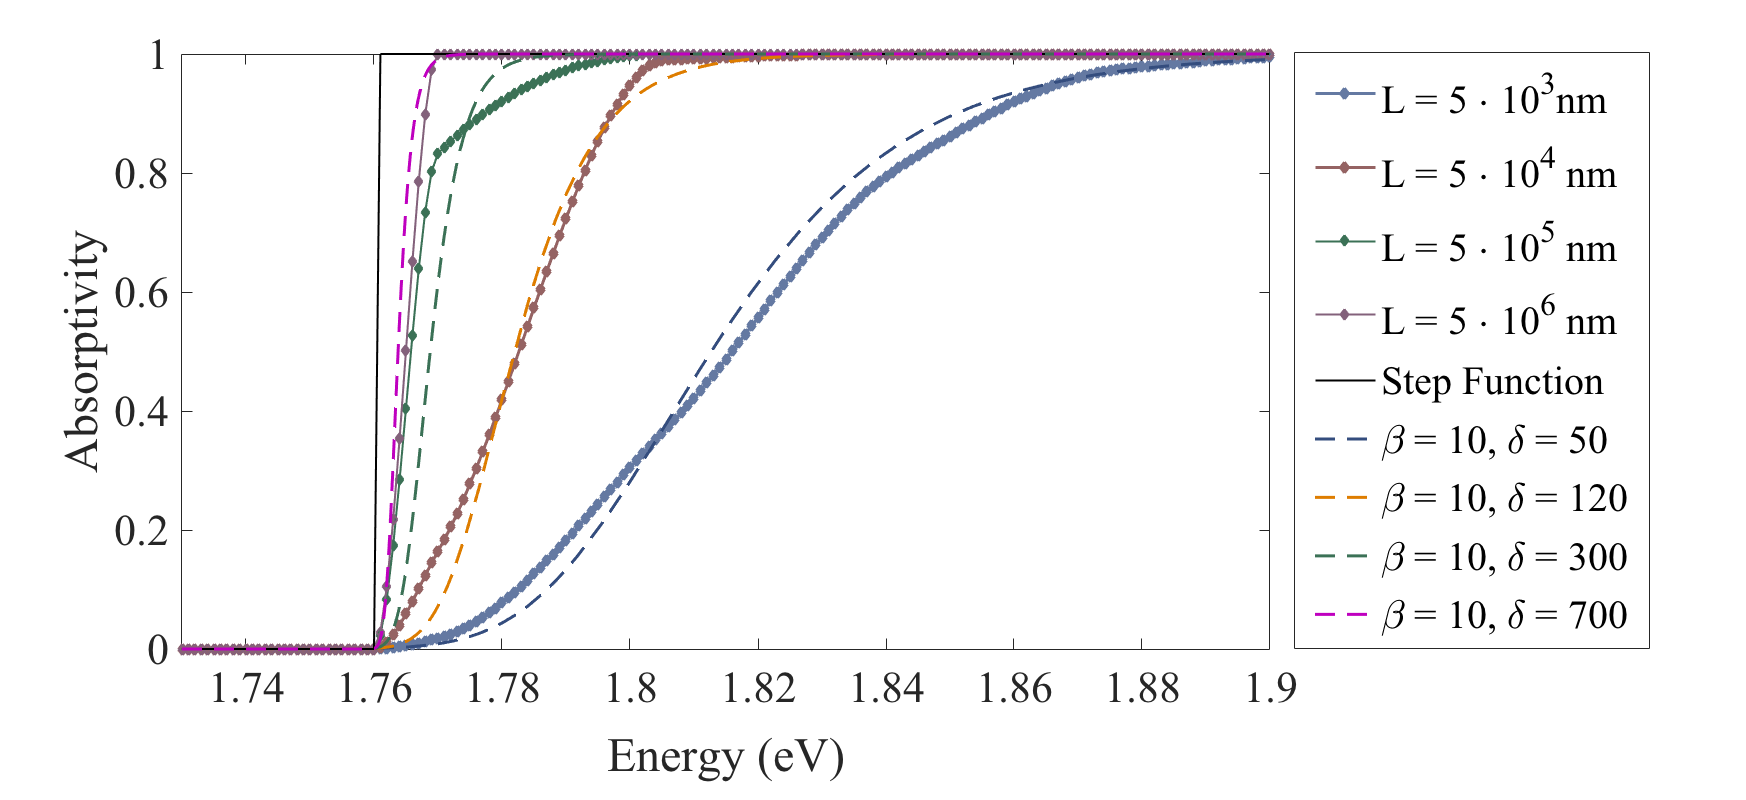
\includegraphics[width=0.9\textwidth]{Figures/slme/sq_Fig2.png} 
\caption{Comparison of the model function with calculated absorptivity spectra 
for \ce{Cu2ZnGeS4} at different thicknesses $L$. The model function shape 
matches that of the calculated absorptivity quite well as $L,\delta 
\rightarrow \infty$.} 
\label{slme:fig-step} 
\end{figure} 
 
To study the influence of the band gap on the likelihood of the efficiency 
exceeding the Shockley-Queisser limit, we calculate the efficiency for $\delta 
\in [1, 10^4]$ over the band gap range $E_g~\in~[0.3, 3]~\si{\electronvolt}$. 
Figure~\ref{slme:fig-deltadep} presents the $\delta$-dependency of the efficiency for a selection of band gaps. For low band gaps, the 
calculated efficiency crosses the detailed balance limit of the corresponding 
band gap, in order to return to the limit value for $\delta \rightarrow 
\infty$. Since $\delta$ can be related to the thickness of the material, this 
implies that for lower band gap materials, there is a thickness that is 
optimal for the efficiency. Moreover, a clear trend is visible, with the 
efficiency exceeding the Shockley-Queisser limit more as the band gap is 
decreased. This is also clear when looking at the plot for the 
maximum efficiency values in Fig.~\ref{slme:fig-logistic}. 
 
\begin{figure}[ht] 
\centering 
\captionsetup{width=0.9\textwidth}
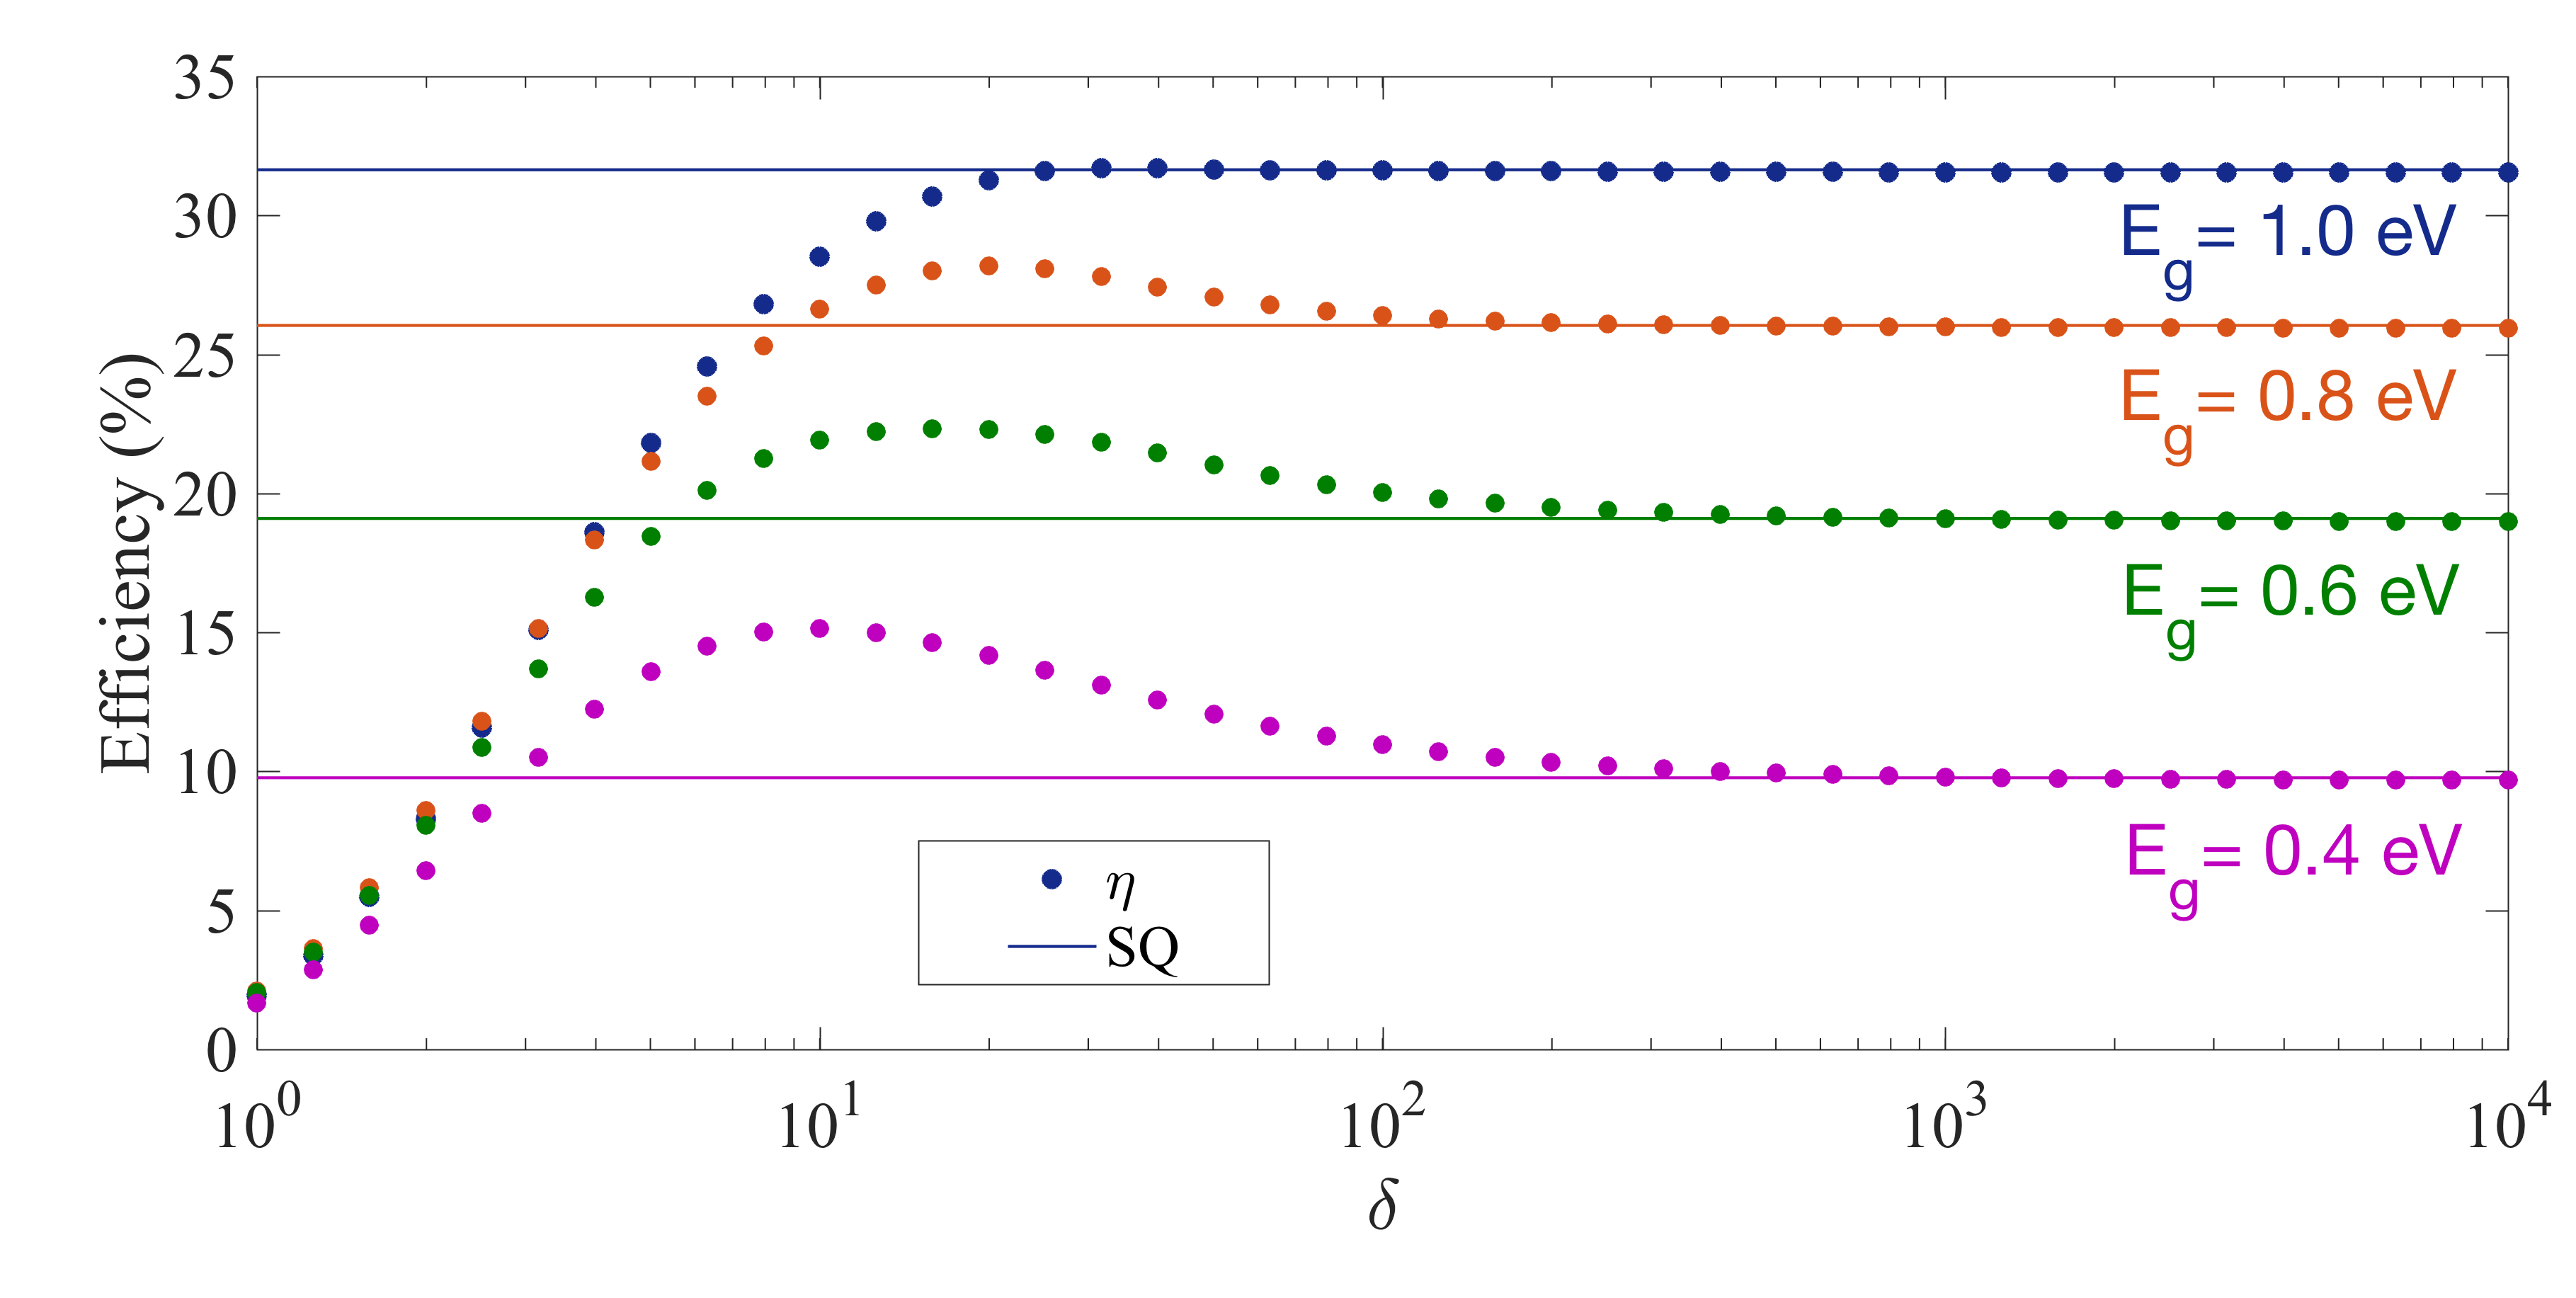
\includegraphics[width=0.8\textwidth]{Figures/slme/sq_Fig3.png} 
\caption{Calculated efficiencies for a range of $\delta$ values and a 
selection of band gaps, compared with the corresponding Shockley-Queisser 
limit.} 
\label{slme:fig-deltadep} 
\end{figure} 
 
Finally, it is interesting to note that the SLME values of the materials that 
exceed the Shockley-Queisser limit are still below the maximum efficiency for 
the model absorptivity functions of the corresponding band gap in 
Fig.~\ref{slme:fig-logistic}. However, this does not imply that the logistic 
function maxima curve represents a new upper limit. It is entirely possible 
that there is another function profile that would allow for higher 
efficiencies. Using the logistic function approach, we are simply able to 
observe for which band gap range the Shockley-Queisser limit does not provide 
a theoretical upper limit within the detailed balance approach. 
 
\resultsubsection{Indirect band gap absorbers \label{slme:sec-indirect}}{https://github.com/mbercx/phd-thesis/blob/master/jupyter/slme/README.md\#indirect-band-gap-absorbers}{}
 
So far, I have only discussed materials which have a direct band gap. In 
order to test the application of the SLME to indirect band gap absorbers, we 
decided to calculate the SLME of silicon, which is still one of the most 
popular materials for the production of solar cells. 
Fig.~\ref{slme:fig-Si_expAbs} shows the experimental\footnote{We choose to 
use an experimental spectrum in order to include the phonon-mediated 
contributions to the absorption coefficient.} absorption coefficient of 
crystalline silicon~\cite{green2008}. Notice the onset of the indirect and 
direct absorption at \mbox{$E_g = 1.17~\si{\electronvolt}$} and 
\mbox{$E_g^{da} = 3.4~\si{\electronvolt}$}, respectively. 

\begin{figure}[ht] 
\centering 
\captionsetup{width=0.9\textwidth}
\includegraphics[width=0.7\textwidth]{\figurepath/slme/absorption_Si.png} 
\caption{Experimental absorption coefficient at $T = 300~\si{\kelvin}$ of 
crystalline silicon with data taken from~\cite{green2008}.} 
\label{slme:fig-Si_expAbs} 
\end{figure} 

Calculating the SLME using this optical spectrum produces an efficiency of 
zero for any thickness $L$ and temperature $T$. The origin of this troubling result is 
rooted in the fraction of radiative recombination expressed in 
Eq.~(\ref{slme:eq-fraction}). Because of the large difference between the 
direct allowed and fundamental band gap of silicon ($\Delta = 
E_g^{da}-E_g=2.23$~\si{\electronvolt}), the radiative fraction is of the order 
$10^{-38}$. Since this fraction is used to calculate the recombination 
current (see Eq.~(\ref{slme:eq-currents})), this results in a $J_0$ that is 
unreasonably large. As discussed in Section~\ref{slme:sec-CuInSe2}, $J_0$ has a 
significant influence on the open circuit voltage $V_{oc}$. In this case, the 
high value of $J_0$ leads to a $V_{oc}$ that is too small to produce any 
significant power density. However, in case the fraction of radiative recombination is set \mbox{$f_r = 10^{-3}$} -- a 
more reasonable value for silicon~\cite{Shockley1952,Trupke2003,Richter2012} -- the results shown in Fig.~\ref{slme:fig-SLME_Si} are obtained. 
 
\begin{figure}[ht] 
	\centering 
		\includegraphics[width=0.7\textwidth]{\figurepath/slme/slme_Si.png} 
	\caption{Thickness dependence of the SLME of silicon.} 
	\label{slme:fig-SLME_Si} 
\end{figure} 
 
One could argue that silicon is a special case, and that generally efficient 
indirect absorbers do not have such a large band gap difference \mbox{$\Delta 
= E_g ^{da}- E_g$}. For thin-film solar cells, indirect absorption also 
contributes significantly less to the power density. Consequently, indirect 
band gap materials with a large fundamental band gap are not suitable for 
these applications in any case. However, even for materials with a small 
$\Delta$, the modeled fraction of radiative recombination quickly becomes 
minute. For example, consider the compound Cu$_3$TlSe$_2$, which has been 
investigated by Yu and Zunger~\cite{Yu2012}. The reported difference between 
the fundamental and direct allowed band gap is $0.24$~\si{\electronvolt}. At 
300~\si{\kelvin}, the fraction of radiative recombination then becomes 
\mbox{$f_r = 10^{-4}$}. This means that although $99.99$~\% of the 
recombination is non-radiative in nature, the recombination current is 
still derived from an entirely radiative principle, based on the black-body 
spectrum in Eq.~(\ref{slme:eq-currents}). Furthermore, it is clear that 
because of the exponential function in Eq.~(\ref{slme:eq-fraction}), the 
fraction of radiative recombination drops very rapidly with increasing 
$\Delta$. This indicates that even for materials with a relatively low 
$\Delta$, the recombination current will rise significantly, which is 
detrimental for the calculated efficiency. Hence, it is entirely possible that 
the recombination model of the SLME metric does not judge indirect band gap 
absorbers fairly, potentially eliminating good materials during the selection 
procedure.\\ 
 
\section{Conclusions and Outlook} 
 
We have compared the structural and thermodynamic properties of the CA and CH 
phase of the compounds. By analyzing the difference in formation energy of the 
CH and CA phase, we conclude that CA domains are most likely to be present in 
\mbox{CuIn-VI$_2$} compounds, which is in good agreement with experimental 
results. From the calculated optoelectronic properties of the materials, we 
have determined their potential as absorbers for solar cells by applying the 
SLME selection metric. We identify several compounds with a high theoretical 
efficiency in the CA phase, most notably \mbox{CA-CuInS$_2$}, which has a 
significantly higher efficiency than the corresponding CH phase. 
 
After observing an SLME value above the Shockley-Queisser limit for 
\mbox{CA-CuInSe$_2$}, we have performed a detailed analysis to find the origin 
of this result. We find that, within the details balance approach, the reverse 
saturation current $J_0$ approaches its SQ value very slowly for an increasing 
thickness $L$. This causes the SLME to cross the SQ limit for materials with a 
$J_0$ that is relatively high, i.e. materials with a low band gap or at higher 
temperatures. In their 1961 paper, Shockley and Queisser characterized their 
calculated efficiency as an upper limit, because of the assumption that if 
every photon with an energy above the band gap is absorbed, the obtained 
efficiency must be maximal. Although this assumption may seem entirely 
sensible at first glance, it does not consider the fact that it also maximizes 
the recombination current, which is calculated using the detailed balance 
principle. Because an increased recombination current results in a lower efficiency, 
this means that lowering the absorptivity can produce higher efficiencies than 
the Shockley-Queisser limit under the right conditions. By using a model 
absorptivity function, which closely resembles absorptivity spectra calculated 
from first principles, we have shown that this can occur for low band gaps. 
This means that one must take care when dismissing low band gap materials 
based on their Shockley-Queisser limit, for their actual efficiency at certain 
thicknesses might still make them suitable for thin film photovoltaic 
applications. Finally, we have shown that the model that introduces non-radiative 
recombination to the SLME quickly undercuts the efficiency of indirect band 
gap absorbers, as the Boltzmann factor used increases the recombination 
current drastically once the difference between the direct and fundamental 
band gap becomes larger. 

Although the SLME has shown promise as a metric for computational materials design 
of photovoltaic absorber layers, there are still some issues which need to be 
resolved. The SLME could benefit from an improved description of the fraction of 
radiative recombination, especially if it is to be applied to indirect band gap absorbers. 
Moreover, other important effects can be introduced, such as multiple exciton 
generation and photon recycling. Finally, we also note that as the efficiency of 
a solar cell depends heavily on the band gap of a material, calculating the SLME 
based on results from density functional theory calculations still poses the risk 
of serious inaccuracy, especially when the band gap is outside the 1-1.5~\si{\electronvolt} range.

\printbibliography 
\end{refsection} 
